% Options for packages loaded elsewhere
\PassOptionsToPackage{unicode}{hyperref}
\PassOptionsToPackage{hyphens}{url}
%
\documentclass[
  12pt,
]{book}
\usepackage{amsmath,amssymb}
\usepackage{lmodern}
\usepackage{iftex}
\ifPDFTeX
  \usepackage[T1]{fontenc}
  \usepackage[utf8]{inputenc}
  \usepackage{textcomp} % provide euro and other symbols
\else % if luatex or xetex
  \usepackage{unicode-math}
  \defaultfontfeatures{Scale=MatchLowercase}
  \defaultfontfeatures[\rmfamily]{Ligatures=TeX,Scale=1}
  \setmainfont[]{Times New Roman}
\fi
% Use upquote if available, for straight quotes in verbatim environments
\IfFileExists{upquote.sty}{\usepackage{upquote}}{}
\IfFileExists{microtype.sty}{% use microtype if available
  \usepackage[]{microtype}
  \UseMicrotypeSet[protrusion]{basicmath} % disable protrusion for tt fonts
}{}
\makeatletter
\@ifundefined{KOMAClassName}{% if non-KOMA class
  \IfFileExists{parskip.sty}{%
    \usepackage{parskip}
  }{% else
    \setlength{\parindent}{0pt}
    \setlength{\parskip}{6pt plus 2pt minus 1pt}}
}{% if KOMA class
  \KOMAoptions{parskip=half}}
\makeatother
\usepackage{xcolor}
\IfFileExists{xurl.sty}{\usepackage{xurl}}{} % add URL line breaks if available
\IfFileExists{bookmark.sty}{\usepackage{bookmark}}{\usepackage{hyperref}}
\hypersetup{
  pdftitle={History of the Piedmont Neighborhood 1850-1920},
  pdfauthor={Jan de Leeuw},
  hidelinks,
  pdfcreator={LaTeX via pandoc}}
\urlstyle{same} % disable monospaced font for URLs
\usepackage{longtable,booktabs,array}
\usepackage{calc} % for calculating minipage widths
% Correct order of tables after \paragraph or \subparagraph
\usepackage{etoolbox}
\makeatletter
\patchcmd\longtable{\par}{\if@noskipsec\mbox{}\fi\par}{}{}
\makeatother
% Allow footnotes in longtable head/foot
\IfFileExists{footnotehyper.sty}{\usepackage{footnotehyper}}{\usepackage{footnote}}
\makesavenoteenv{longtable}
\usepackage{graphicx}
\makeatletter
\def\maxwidth{\ifdim\Gin@nat@width>\linewidth\linewidth\else\Gin@nat@width\fi}
\def\maxheight{\ifdim\Gin@nat@height>\textheight\textheight\else\Gin@nat@height\fi}
\makeatother
% Scale images if necessary, so that they will not overflow the page
% margins by default, and it is still possible to overwrite the defaults
% using explicit options in \includegraphics[width, height, ...]{}
\setkeys{Gin}{width=\maxwidth,height=\maxheight,keepaspectratio}
% Set default figure placement to htbp
\makeatletter
\def\fps@figure{htbp}
\makeatother
\setlength{\emergencystretch}{3em} % prevent overfull lines
\providecommand{\tightlist}{%
  \setlength{\itemsep}{0pt}\setlength{\parskip}{0pt}}
\setcounter{secnumdepth}{5}
\ifLuaTeX
  \usepackage{selnolig}  % disable illegal ligatures
\fi

\title{History of the Piedmont Neighborhood 1850-1920}
\author{Jan de Leeuw}
\date{Started in 2016. Last update September 01, 2021}

\begin{document}
\maketitle

{
\setcounter{tocdepth}{4}
\tableofcontents
}
\begin{figure}
\centering
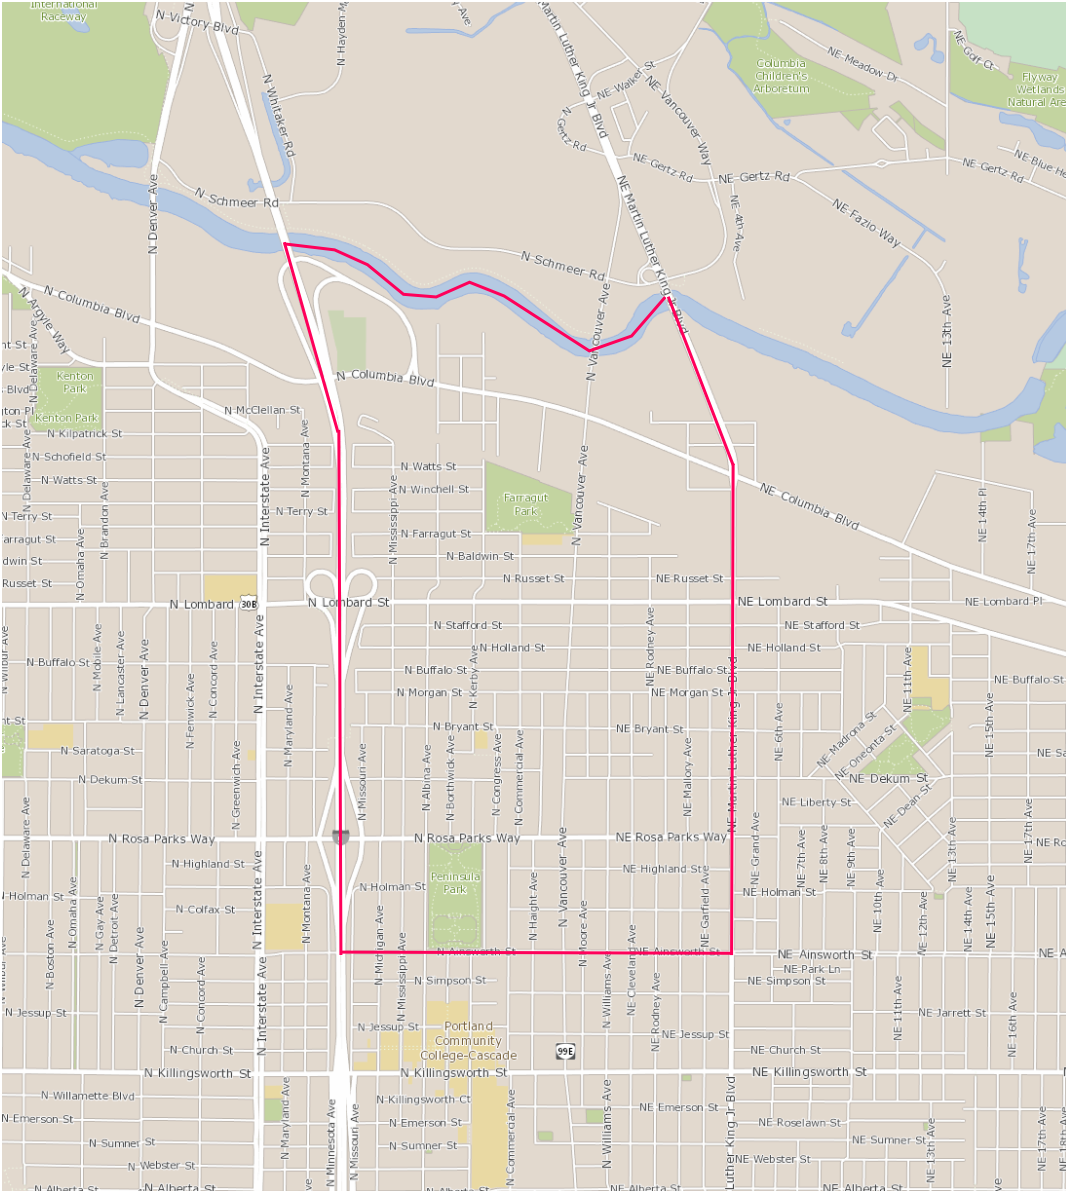
\includegraphics{images/00_images/image1.png}
\caption{alt\_text}
\end{figure}

\hypertarget{introduction}{%
\chapter*{Introduction}\label{introduction}}
\addcontentsline{toc}{chapter}{Introduction}

\hypertarget{piedmont}{%
\section*{Piedmont}\label{piedmont}}
\addcontentsline{toc}{section}{Piedmont}

Piedmont is one of the 95 neighborhoods in the neighborhood system of Portland, Oregon, and one of the eleven neighborhoods in the North Portland district coalition.

\begin{quote}
\emph{Portland's nationally recognized neighborhood system is made up of 95 recognized,
independent neighborhood associations and seven neighborhood district coalition offices
that represent the entire city of Portland.
\url{https://www.portlandoregon.gov/oni/28989}}
\end{quote}

The Piedmont neighborhood gets its name from the Piedmont subdivision, platted in 1889 by Edward Quackenbush and the Investment Company. And the Piedmont subdivision gets its name from the region in northwest Italy, known for its gentle slopes and hillsides. I am pretty sure the name Piedmont was chosen for its commercial appeal, and not for the physical resemblance with the eponymous region in Italy, which actually looks quite different.

Although:\url{https://en.wikipedia.org/wiki/Piedmont_(United_States)}

The Piedmont subdivision is only a small part of the Piedmont neighborhood, in fact less than ten percent of its area. And, conversely, only half of the Piedmont subdivision is in the Piedmont neighborhood, the rest is in Humboldt and King.

\hypertarget{land}{%
\section*{Land}\label{land}}
\addcontentsline{toc}{section}{Land}

Throughout this book, I concentrate on land and land ownership. It is essential, therefore, to remember that Oregon, Portland, and Piedmont were started by settler colonialism. This meant the United States occupied lands used for centuries by indigenous peoples, and declared it to be public lands of the United States. War, terror, vigilantes, disease, broken treaties, racism, religion, and unjust laws made sure the unceded lands stayed in the hands of the occupying forces. The small percentage of indigenous people that survived the onslaught were driven onto ever shrinking reservations. In the middle of the nineteenth century, when settlers started to arrive and Portland became a fast growing city, there were very few Native Americans left in the area.

In that nineteenth century the United States adopted laws which encouraged settlement by giving large sections of public lands away (usually tracts of 160 acres), and making other sections available for very little money (usually for \$ 1.25 per acre). The land that currently makes up Piedmont was donated in this way to just four people. Evander Howe, George Smith, Lewis Love, and David Ulery were all farmers on the Vancouver Road, near the Columbia Slough. They could effectively use the Donation Land Claim Act and the Military Bounty Law, because they were the first settlers to arrive, and actually for quite some time the only settlers to arrive.

In the next stage the city grew because the settlers, or ``pioneers'', sold their land to developers, who platted subdivisions. Piedmont over the years became differentiated from about four homesteads to about 30 subdivisions of varying sizes. From 1850 on fortunes were made by subdividing, exchanging, transfering, inheriting, buying, and selling pieces of land. In the third stage of development each of the subdivisions, sometimes also called additions, were partitioned into a varying number of city blocks, usually 200 by 200 feet, and the blocks were partitioned in lots, usually eight lots of 100 by 50 feet. These individual lots were then sold to people to build their houses, or packaged into multiple lots for speculation. Piedmont consists of thousands of such lots.

In the book I will discuss the original homesteads and the subsequent subdivisions. As a consequence of this emphasis on land, the book concentrates on the time between 1850 and 1930. After 1930 development is mostly down to the level of individual lots, and since there are about 5000 of these, I cannot discuss them one by one. It is interesting, of course, to find out who built an individual house, and who the subsequent owners were. But the sheer number of them makes it impossible to write about each and every one.

\hypertarget{bias}{%
\section*{Bias}\label{bias}}
\addcontentsline{toc}{section}{Bias}

As you will probably figure out quickly, I like maps. I also like facts, more than I like opinions. I like words, more than I like photographs. Thus this book is not of the coffee table type, with many photos and only a few words.

I also do not like the view that historical developments are driven by a small number of important individuals, always men of course, and that we want to know as much as possible about these men, possibly because we want to become just like them. History is driven by social and economic forces and movements in which specific individuals are of limited and largely anecdotal significance. I like to report about structures and systems more than I like to report about people. Also, I hope that what I do report about the men and women that were important in Piedmont's early history makes it clear that you do not necessarily want to become just like them.

There are two other important types of Portland history books I do not want to emulate. Some of them are excellent, but they are not what I am interested in. There are those books that concentrate on vice, corruption, crime, shanghaiing, and prostitution. They are mostly about the northwest of Portland, between 1870 and 1910. And then there are those books that tell the story of city government and the business community, again mostly although not entirely about the part of Portland west of the river. As far as I am concerned, these two types of books talk about two sides of the same coin, a bunch of people quibbling on how to divide the loot. Of course that describes a huge part of history in general, and in this book the loot is basically two square miles of land, sections 10 and 15 in township one north, range one east of the Willamette Meridian.

\hypertarget{technical}{%
\section*{Technical}\label{technical}}
\addcontentsline{toc}{section}{Technical}

This book is, and always will be, free and in the public domain. Anyone can copy, print, distribute or otherwise use the material in this book for any purpose whatsoever, and, if they so choose, without attribution.

All references are collected in the back of each chapter or section. I have tried to make everything reproducible, in the sense that every statement of fact that I make can be traced back to its sources. I have also tried to emphasize primary (i.e.~contemporaneous) sources, even if they were only newspaper articles. Secondary sources are only used, reluctantly, if primary sources are not available. I have also tried to refrain, as much as is humanly possible, from stating opinions about events, or making inferences about motives.

This book is a living document, which means that any part of it can change at any moment. Thus all sections have a date attached to their title, indicating when they were last changed. I keep discovering new facts and adding new materials. In the table of contents each section is linked to a separate pdf, which is synchronized with the sections in the Google docs version of the book.

This book is also, among other things, a repository. There are copies of, or links to, the original maps, deeds, photos, and newspaper articles that the narrative is based on. If you see a link below a figure or a map, then following that link will usually get you to a bigger and better version of the map you can either download to your computer or view in your browser. Generally you get the best resolution by downloading the file and opening it in the appropriate application.

\hypertarget{references}{%
\section*{References}\label{references}}
\addcontentsline{toc}{section}{References}

The City of Portland, Oregon. \emph{Neighborhood Program}
\url{https://www.portlandoregon.gov/oni/28989}

Alta Mitchoff: \emph{History of the Kenton Neighborhood}
Kenton Neighborhood Association, 1997

Anjala Ehelebe: \emph{Portland's Woodlawn Neighborhood}
Arcadia Publishing, 2008

Roy E. Roos: \emph{The History and Development of Portland's Irvington Neighborhood}
Self published, 1997

Roy E. Roos: \emph{The History of Albina. Including Eliot, Boise, King, Humboldt, and Piedmont Neighborhoods}
Self published, 2008

\hypertarget{they-were-here-first.-and-they-are-still-here.}{%
\chapter{They Were Here First. And They Are Still Here.}\label{they-were-here-first.-and-they-are-still-here.}}

\begin{figure}
\centering
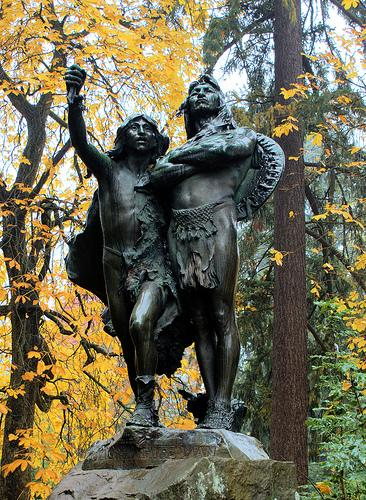
\includegraphics{images/01_images/image1.jpg}
\caption{alt\_text}
\end{figure}

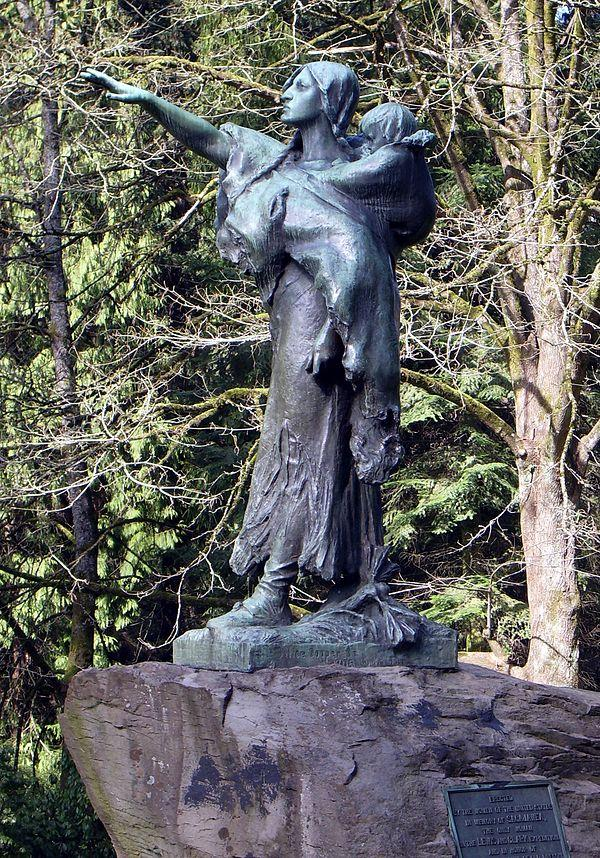
\includegraphics{images/01_images/image2.jpg}
\#\# Introduction

They made us many promises, more than I can remember.

But they kept only one -- They promised to take our land \ldots{} and they took it.

Red Cloud, Lakota, around 1900

It is appropriate to start this book with a chapter on the Native Americans who were here first and who lived on the land that is currently the Piedmont Neighborhood. It turns out that this is far from easy. I will have to rely heavily on a huge amount of research on relatively sparse data, documented most thoroughly in an excellent recent edited volume.

Robert T. Boyd, Kenneth M. Ames, Tony A. Johnson (eds): \emph{Chinookan Peoples of the Lower Columbia.} University of Washington Press, 2013.

To set the scene we start with two statues in Washington Park. The first one, on the left, is called ``\emph{The Coming of the White Man}''. The sculptor was Hermon Atkins MacNeil (1866 -- 1947), who specialized in Native American scenes. This particular statue was gifted to the City of Portland in 1904 by former mayor \href{https://en.wikipedia.org/wiki/David_P._Thompson}{David P. Thompson}. It depicts two Native American men looking towards the \href{https://en.wikipedia.org/wiki/Columbia_River}{Columbia River} upon the arrival of \href{https://en.wikipedia.org/wiki/Lewis_and_Clark_Expedition}{Lewis and Clark}. The older man, with arms crossed, is supposedly Chief Multnomah, the younger one is not identified. Sculptor MacNeil continued to make and sell many separate copies of the Chief Multnomah figure.

There are some problems with the statue, independent of its artistic merits. First, there is a relatively minor historical problem. For a long time historians have denied that Chief Multnomah was an actual historical figure. Recent research (Fulton, 2005), relying on the native american oral tradition, maintains that he did indeed exist. He was a powerful and important chief, who controlled a large territory around the Willamette river, and commanded many warriors. He died around 1780, possibly in the first smallpox epidemic. Whether he existed or not, he was no longer living when Lewis and Clark arrived in 1804-1805.

The second problem, which was unavoidable at the time, is that the statue is firmly in the white supremacist tradition of the Noble Savage, the Theatrical Savage, and the Picturesque Savage (Ellington, 2001). A good way to illustrate this is with a contemporary review of the statue by one Arno Dosch in the Pacific Monthly of 1905.

\begin{quote}
Mr.~MacNeil has put thought and genius into that old chief. He has depicted a patriarch in the full possession of his bodily strength, with a frame of iron, legs of steel cords and an arm of certain stroke. He stand on his toes to see better, binding his knees with tendons and drawing the cords over his thighs, hollowing the hips and bringing out the groin line clear. His are the legs of perfect strength, with the veins showing a little more prominently than in a younger man. On an upright body, with arms folded and a shield slung over the back, rises the head. In the face is the power. It is that of a Multnomah, a man of mental ability, a brooding savage, an Indian chief. He guided his own people by his wisdom, and let them in conquest on the enemy. The neck is drawn in heavy cords, and upon it is the chin of hauteur, almost disdain, the eyes expectant, but not astonished; the nose masterful, the strong hair bound back by a band.\_
\end{quote}

The younger person is also described by Dosch.

\begin{quote}
\emph{His attitude is in direct contrast to that of his elder. His whole body and face expresses open curiosity and wonderment. He holds aloft on his right hand a branch, just broken from a tree, and waves it as a token of good will to the strangers.}
\end{quote}

At some point in time in the 1930's someone, presumably someone with a more keen sense of history, broke off this olive branch from the statue. It has not been restored.

Remember that Arno Dosch wrote in 1905. In the preceding 100 years an estimated ninety percent of the Native American population had disappeared. They largely succumbed to diseases brought by the white man. But they had also been hunted down and killed by vigilantes and slaughtered in staged so-called ``Indian Wars'' by the army. They were driven from their lands, tricked into signing treaties that would never be ratified, and they were forcibly removed to areas east of the Cascades, or driven onto small reservations of land that the white settlers did not want. In 1905 the expression on the face of Chief Multnomah should have alternated between immense sadness and equally immense rage.

The second statue in Washington Park, the picture on the right, is ``\emph{Sacajawea and Jean-Baptiste}''. The sculpture was commissioned for the \href{https://en.wikipedia.org/wiki/Lewis_and_Clark_Centennial_Exposition}{Lewis and Clark Centennial Exposition} (1905) by the Committee of Portland Women, who requested a sculpture of ``\emph{the only woman in the Lewis and Clark Expedition and in honor of the pioneer mother of old Oregon}.''

\hypertarget{before-contact}{%
\section{Before Contact}\label{before-contact}}

Archeology

\hypertarget{discovering-the-columbia}{%
\section{Discovering the Columbia}\label{discovering-the-columbia}}

\hypertarget{the-lewis-and-clark-journals}{%
\section{The Lewis and Clark Journals}\label{the-lewis-and-clark-journals}}

The two visits to Native American sites in the Columbia Basin/Wapato Valley

\hypertarget{the-wapato-valley-native-americans}{%
\section{The Wapato Valley Native Americans}\label{the-wapato-valley-native-americans}}

\hypertarget{the-spirit-of-pestilence}{%
\section{The Spirit of Pestilence}\label{the-spirit-of-pestilence}}

\hypertarget{the-extinction-of-indian-title}{%
\section{The Extinction of Indian Title}\label{the-extinction-of-indian-title}}

How the lands were taken away (In the Courts of the Conqueror, Conquest by Law).

\begin{quote}
\emph{There has been some discussion as to the origin of our title to what was known as the Oregon country, comprising the State of Oregon, Washington and Idaho, and the portions of Montana and Wyoming west of the Rocky Mountains. The question wa whether our title was derived from the Louisiana Purchase or directly by discovery and prior possession. As the result of discussion by the General Land Office in 1898, the map of the United States now issued by that office states that the title was established in 1846. The exact basis of our claim has apparently never been authoritatively decided (Bien, 1910, page 388).}
\end{quote}

\hypertarget{present-day-multnomah-county}{%
\section{Present Day Multnomah County}\label{present-day-multnomah-county}}

\hypertarget{references-1}{%
\section{References}\label{references-1}}

Morris Bien: \emph{The Public Lands of the United States.}
The North American Review, 192, 1910, 387-402
\url{https://drive.google.com/file/d/1TT_lgoh_nI8LSdztGw_claFQYfHje16G}

Jerry A. O'Callaghan: \emph{The Disposition of the Public Domain in Oregon}
Dissertation submitted to the Department of History and the Committee on Graduate Study of Stanford University, November 1960
\url{https://drive.google.com/file/d/1T8HRj39qobQ_4NkydJpagwnRQvFPAEUB}

Gary E. Moulton (ed): \_The Lewis and Clark Journals. An American Epic of Discovery. The Abridgment of the Definitive Nebraska Edition. \_University of Nebraska Press, 2004

Gary E. Moulton (ed): \_The Definitive Journals of Lewis \& Clark. Down the Columbia to Fort Clatsop. \_Volume 6 of the Nebraska Edition. University of Nebraska Press, 1990.

Gary E. Moulton (ed): \_The Definitive Journals of Lewis \& Clark. From the Pacific to the Rockies. \_Volume 7 of the Nebraska Edition. University of Nebraska Press, 1991.

Robert T. Boyd, Kenneth M. Ames, Tony A. Johnson (eds): \emph{Chinookan Peoples of the Lower Columbia.} University of Washington Press, 2013.

Michael Silverstein: \_Chinookians of the Lower Columbia. \_In Wayne Suttles (ed): \emph{Handbook of North American Indians, Volume 7, Northwest Coast}, p 533-546. Washington, Smithsonian, 1990.

Robert H. Ruby and John A. Brown: \_The Chinook Indians. Traders of the Lower Columbia River. \_University of Oklahoma Press, Norman, Oklahoma, 1976.

Robert H. Ruby, John A. Brown, Cary C. Collins: \emph{A Guide to the Indian Tribes of the Pacific Northwest.} University of Oklahoma Press, Norman, Oklahoma, Third Edition, 2010.

Ann Curry-Stevens, Amanda Cross-Hemmer, Coalition of Communities of Color:\_ The Native American Community in Multnomah County. An Unsettling Profile. \_Portland State University, School of Social Work, 2011. \url{https://pdxscholar.library.pdx.edu/cgi/viewcontent.cgi?article=1093\&context=socwork_fac}

Robert A. Williams, Jr: \emph{The American Indian in Western Legal Thought.} \_The Discourses of Conquest. \_Oxford University Press, 1990

Robert A. Williams, Jr: \emph{Savage Anxieties.} \_The Invention of Western Civilization. \_Palgrave McMillan, 2012

Ann Fulton: \_The Restoration of Iłkák'mana: A Chief Called Multnomah. \_American Indian Quarterly, 31, 2007, 110-128

Ter Ellington: \emph{The Myth of the Noble Savage}. University of California Press, 2001.

Lindsay G. Robertson: \_Conquest by Law. How the Discovery of America Dispossessed Indigenous People of their Lands. \_Oxford University Press, 2005

Walter R. Echo-Hawk: \_In the Courts of the Conqueror. The 10 Worst Indian Law Cases Ever Decided. \_Fulcrum Publishing, 2012.

Arno Dosch: \_The Coming of the White Man. \_The Pacific Monthly, 13, 1905, 50-52

The Native American Community in Multnomah County:

\hypertarget{homesteaders-and-homesteads}{%
\chapter{Homesteaders and Homesteads}\label{homesteaders-and-homesteads}}

\hypertarget{introduction-1}{%
\section{Introduction}\label{introduction-1}}

\begin{figure}
\centering
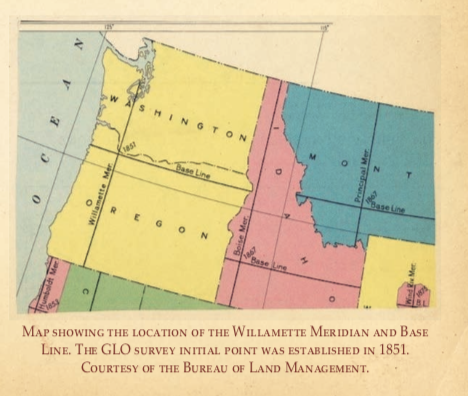
\includegraphics{images/02_images/image1.png}
\caption{alt\_text}
\end{figure}

\hypertarget{the-map}{%
\subsection{The Map}\label{the-map}}

The map above shows those donation lands and homesteads the United States handed out and sold around 1850-1860 that cover the Piedmont neighborhood (which is the area within the red boundaries). There is only a small number of them, five or so, and the large parcels (in the blue lines) in most cases also overlap with the adjacent neighborhoods Woodlawn, Overlook, Humboldt, King, Arbor Lodge, Kenton, and East Columbia. I shall use the generic name ``homesteads'' for these properties, although not all of them were authorized by the homestead act, and not all the original grantees actually homesteaded on them.

To put this in a larger context, here is the map of the 1860 survey of all of Township 1 of Range 1 east, which covers all of Portland, including East Portland and Albina.

\begin{figure}
\centering
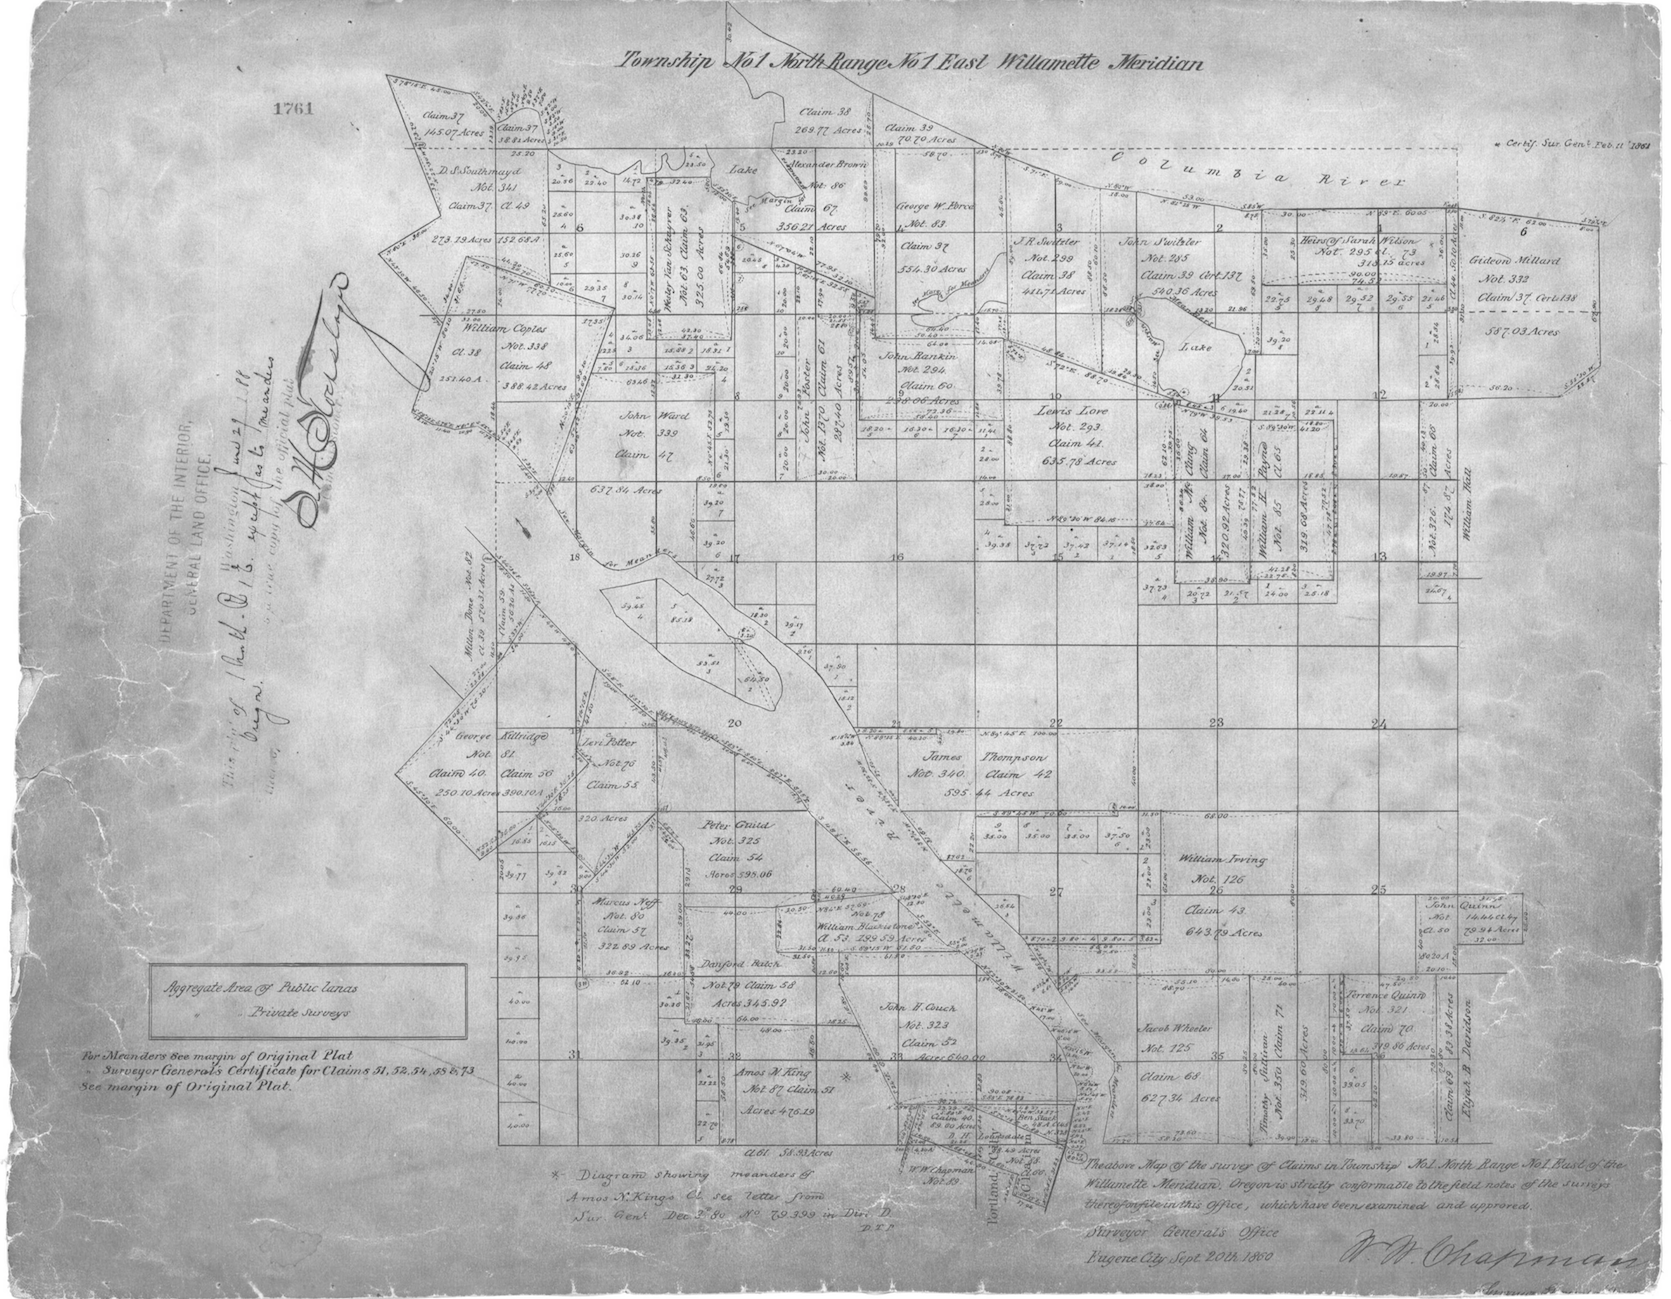
\includegraphics{images/02_images/image2.png}
\caption{alt\_text}
\end{figure}

\url{https://drive.google.com/file/d/1TISCAUaStTYOVqZS58E5ao4AFFOkmzSl}

Remember that links in the captions below pictures and photos generally point to a larger and/or higher resolution version elsewhere on the web. On the map it says, in the lower right hand corner,

\begin{quote}
The above Map of the Survey of Claims in the Township No1 North Range No1 East of the Willamette Meridian, Oregon, is strictly conformable to the field notes of the surveys thereof in file at this office, which have been examined and approved.
Surveyor General's Office, Eugene City, September 20th 1860
\end{quote}

The township and range terminology will be discussed later in this introductory chapter, in the section on the Public Land Survey System.

\hypertarget{our-discussion}{%
\subsection{Our Discussion}\label{our-discussion}}

Each of our homestead chapters is divided into two parts. In the first part I discuss the land, how it was obtained, partitioned, and sold. In the second part I discuss the biographical information I have on the settlers who claimed the land and obtained the patents from the US government. The order of the two parts reflects the emphasis in this book on the ownership of the land, the persons are in some sense accidental, no matter how interesting their lives may have been. But sometimes the division between the land dealings and the life are somewhat artificial, because basically what we know about some of the homesteaders is precisely that they homesteaded in what is now the Piedmont neighborhood. And not much more.

How the land changed hands covers a period from the original claim to the point, often some fifty years later, when the final subdivisions were platted and the plats recorded with Multnomah County. Some plats have hundreds of lots, and it is not feasible to find out and document how individual lots were sold by the original sellers, and then later by the various owners along the way. So I stop at the subdivision level, although there are some exceptions because there is land that was not platted, and there are some lots and buildings on the land with historical significance.

Snyder's 1989 book ``\emph{We Claimed This Land: Portland Pioneer Settlers}'' is impressive, because it covers 212 ``pioneers'', defined as persons or families who ``were the first to settle on the land that is now occupied by the city of Portland, Oregon.'' (1989, preface, page v). But 212 biographies in a book of 278 pages implies that some of them will be very short. Especially because some of the pioneers do get a lot of pages. A. P. Dennison, for example, inexplicably gets 22 pages, which is definitely not proportional to his historical importance. Moreover, Snyder concentrates on pioneers associated with the original site of the City of Portland, on the west side of the Willamette, and on the more urban tracts. This makes perfect sense, because information about them is more readily available. Our Piedmont pioneers Evander Howe (10 lines), George Smith (9 lines), and David Ulery (12 lines) are given short shrift, simply because Snyder does not have more information on them. And some of the information is incorrect or imprecise. Captain Lewis Love gets three pages, which is still not much for such a long and eventful life. John Fenstermacher gets a full page, but mostly because of the tabloid aspects of his life and death. Because we only have to consider just four or five pioneers we can dig much deeper, and find more (and more correct) information.

We freely use the words ``pioneers'' and ``settlers'', although both words have plenty of negative connotations these days (Sakai, 2014). The words seem to suggest that the white people who came from the east arrived on virgin land (the terra nullius doctrine), which was waiting to be occupied, utilized, monetarized, and exploited. The alternative interpretation of what took place in the early nineteenth century is, of course, that all that land was invaded and occupied, and the original inhabitants, the ones that did not succumb to the infectious diseases brought by the settlers, were forcibly removed and in many instances killed. As a rule the white settlers seem to have been brave, daring, inventive, hard working, and incredibly resistant to many kinds of adversity. They came to improve their situation, and many who came early succeeded in doing just that. Their improvement was made possible, however, by the racism, exceptionalism, and manifest destiny ideologies promoted by the ruling classes. And we should not forget they were, wittingly or unwittingly, part of a racist and colonialist invasion that resulted in an horrific genocide (Dunbar-Ortiz, 2014)

\hypertarget{land-laws}{%
\subsection{Land Laws}\label{land-laws}}

There were multiple laws passed by Congress in the eighteenth and nineteenth century on which the various donations and patents are based. Some of them were actually donations, which means the settlers did not have to pay anything for the land, and some were for-pay, although always for very little money.

Because nothing beats looking at the original documents, in the exact language they were written in, I provide links to the actual laws. In the references at the end of the chapter there are links to Wikipedia articles that provide at least some background. If you want to know more about how the United States disposed on its public lands through a whole sequence of homestead type acts, there is the authoritative article by \href{https://drive.google.com/file/d/1TT_lgoh_nI8LSdztGw_claFQYfHje16G}{Bien (1910)}. For an even more extensive discussion of the donations of various types in Oregon (including giveaways to railroads, timber harvesting, or military wagon roads) see the dissertation by \href{https://drive.google.com/file/d/1T8HRj39qobQ_4NkydJpagwnRQvFPAEUB}{Jerry O'Callaghan (1951)}.

\emph{September 27, 1850: An Act to create the Office of Surveyor-General of the Public Lands in Oregon, and to provide for the Survey, and to make Donations to Settiers of the said Public Lands. \url{https://drive.google.com/file/d/1S69AEHN-PuDvYEKimOUQxD4bzhTkTBSd}}

March 3, 1855: \emph{An Act in Addition to certain Acts granting Bounty Land to certain Officers and Soldiers who have been engaged in Military Service of the United States. }\href{https://drive.google.com/file/d/1Ro5Zk00kgc0UpUnpt7aUpvw05e0H0X6b/view}{https://drive.google.com/file/d/1Ro5Zk00kgc0UpUnpt7aUpvw05e0H0X6b}.

May 20, 1862: An Act to secure Homesteads to actual Settlers in the Public Domain. \url{https://drive.google.com/file/d/1S1TuL2j2sMidQAdCahzAFG4hSx27SkhV}

On the map at the beginning of this chapter Lewis Love and John Rankin used the Oregon Donation Land Act of 1850. John Fenstermacher and Evander Howe used the Homestead Act of 1862 (which means they had to pay for their land). George Smith, Robert Maxey, and David Ulery used the Military Bounty Act of 1855. In all three cases, however, they were not the ones doing the actual military service. By informal and and by now unknowable transactions they made the original military men sign over their patents, undoubtedly for a pittance.

The Oregon Donation Land Act of 1850 deserves some additional attention, because it is specific to our region. The \href{https://drive.google.com/file/d/0B94Urj3OjM7BcWhIYmUtV0htcms}{Genealogical Forum of Oregon (2014)} has a nice brochure, with the essential facts. Also quite readable is the page on the act of the\href{https://oregonhistoryproject.org/articles/historical-records/oregon-land-donation-claim-notification/\#.WriRZS-ZPDY}{Oregon History Project (2018)}.

\hypertarget{public-land-survey-system}{%
\subsection{Public Land Survey System}\label{public-land-survey-system}}

The \_Rectangular Survey System** **\_was created by the Land Ordinance of 1785. It covers the United States with squares of 6 by 6 miles. It then introduces a local coordinate system by designating a vertical lines (meridian) and horizontal line (base line). In our case the vertical line is the Willamette Meridian, running through the hills west of Portland, and the horizontal line is the Willamette base line, along Base Line Street (now Stark Street). The two intersect at the \href{https://en.wikipedia.org/wiki/Willamette_Stone}{Willamette Stone}. This local coordinate system allows one to code the squares, indicating how many squares east or west of the meridian, and how many squares north or south of the base line they are. The figure below, taken from page 25 of the \href{https://www.blm.gov/or/landsrealty/glo200/files/glo-book.pdf}{excellent e-book by Vaughan (2014)}, show both meridian and base line.

\begin{figure}
\centering
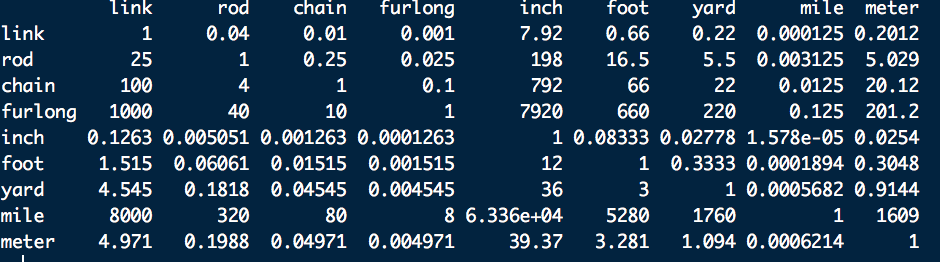
\includegraphics{images/02_images/image3.png}
\caption{alt\_text}
\end{figure}

On the map at the beginning of this chapter you see modern Piedmont in the red boundaries. The black squares are sections 9, 10, 15, and 16 of Township 1 North, Range 1 East (T 1N R 1E), i.e.~the first square north of the baseline and east of the meridian.

A township in PLSS is six by six miles, with 36 sections. Thus T 1N R 1E covers most of Portland. A black section is a square mile, or 640 acres, and the four quarters of a section (NE, SE, SW, NW) are each 160 acres. The following figure, from page 28, of \href{https://www.blm.gov/or/landsrealty/glo200/files/glo-book.pdf}{Vaughan (2014)}, illustrates the basics.

\begin{figure}
\centering
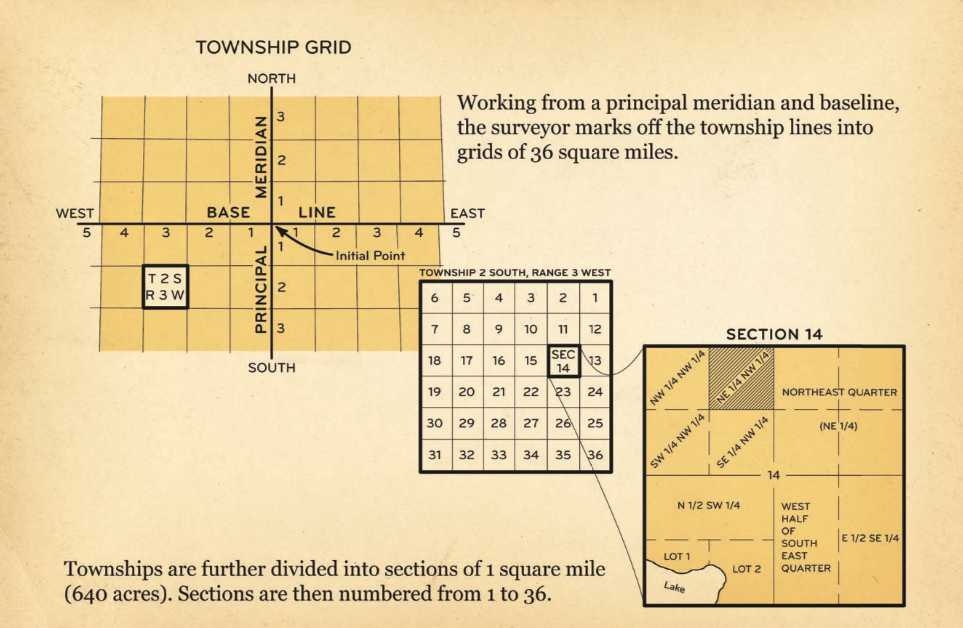
\includegraphics{images/02_images/image4.png}
\caption{alt\_text}
\end{figure}

The rectangular system is used throughout to locate parcels of land, where basically each of the townships provides another even more local coordinate system. We can now say, for example, that a piece of land in the figure above is the SE ¼ of the NW quadrant of Section 14 in township 4 south of range 3 west. Even more importantly, parcels of land, especially in the homestead period, are often defined as sections or quarters of the system, and as a consequence roads often align with boundaries of quarters as well.

\hypertarget{surveyors-lengths}{%
\subsection{Surveyors Lengths}\label{surveyors-lengths}}

In many of the deeds from the nineteenth century parcels of land are described in the language of surveyors, and the boundaries are described in the units of length used by surveyors around that time. Since these units may be unfamiliar to modern readers, I briefly summarize definitions of the most common ones, and show how to translate them into feet and even meters.

\begin{verbatim}
_The name **furlong** derives from the [Old English](https://en.wikipedia.org/wiki/Old_English_language) words furh (furrow) and lang (long). Dating back at least to early [Anglo-Saxon](https://en.wikipedia.org/wiki/Anglo-Saxon) times, it originally referred to the length of the furrow in one [acre](https://en.wikipedia.org/wiki/Acre) of a ploughed [open field](https://en.wikipedia.org/wiki/Open-field_system) (a medieval communal field which was divided into strips). _


_A **chain** is a [unit](https://en.wikipedia.org/wiki/Units_of_measurement) of [length](https://en.wikipedia.org/wiki/Length) that measures 66 [feet](https://en.wikipedia.org/wiki/Foot_(unit)), 22 [yards](https://en.wikipedia.org/wiki/Yard_(unit_of_length)), 100 [links](https://en.wikipedia.org/wiki/Link_(unit)),<sup> </sup>or 4 [rods](https://en.wikipedia.org/wiki/Rod_(unit)) (20.1168 [m](https://en.wikipedia.org/wiki/Metre)). There are 10 chains in a [furlong](https://en.wikipedia.org/wiki/Furlong), and 80 chains in one [statute mile](https://en.wikipedia.org/wiki/Statute_mile). An [acre](https://en.wikipedia.org/wiki/Acre) is the area of 10 square chains (that is, an area of one chain by one furlong). _


_The **rod** or perch or pole is a [surveyor’s](https://en.wikipedia.org/wiki/Surveying) tool<sup> </sup>and unit of [length](https://en.wikipedia.org/wiki/Length) equal to ​5 <sup>1</sup>⁄<sub>2</sub> [yards](https://en.wikipedia.org/wiki/Yard), 16​<sup>1</sup>⁄<sub>2</sub> [feet](https://en.wikipedia.org/wiki/Foot_(length)), ​<sup>1</sup>⁄<sub>320</sub> of a [statute mile](https://en.wikipedia.org/wiki/Statute_mile) or one-fourth of a [surveyor's chain](https://en.wikipedia.org/wiki/Chain_(unit)) and 5.0292 [meters](https://en.wikipedia.org/wiki/Meter). The rod is useful as a unit of length because whole number multiples of it can form one [acre](https://en.wikipedia.org/wiki/Acre) of square measure. _


_The **link** (usually abbreviated as "l.", "li." or "lnk."), sometimes called a **Gunter’s link**, is a [unit](https://en.wikipedia.org/wiki/Physical_unit) of [length](https://en.wikipedia.org/wiki/Length) formerly used in many English-speaking countries. A link is exactly ​<sup>66</sup>⁄<sub>100</sub> of a [foot](https://en.wikipedia.org/wiki/Foot_(unit)), or exactly 7.92 [inches](https://en.wikipedia.org/wiki/Inch) or 20.1168 cm.The unit is based on [Gunter's chain](https://en.wikipedia.org/wiki/Gunter%27s_chain), a metal [chain](https://en.wikipedia.org/wiki/Chain_(unit)) 66 feet long with 100 links, that was formerly used in land [surveying](https://en.wikipedia.org/wiki/Surveying)._
\end{verbatim}

Here is a table to convert links/chains/rods/furlongs to inches/feet/yards/miles and ultimately, for those of us who finally emerged from the middle ages, to meters.

\begin{figure}
\centering
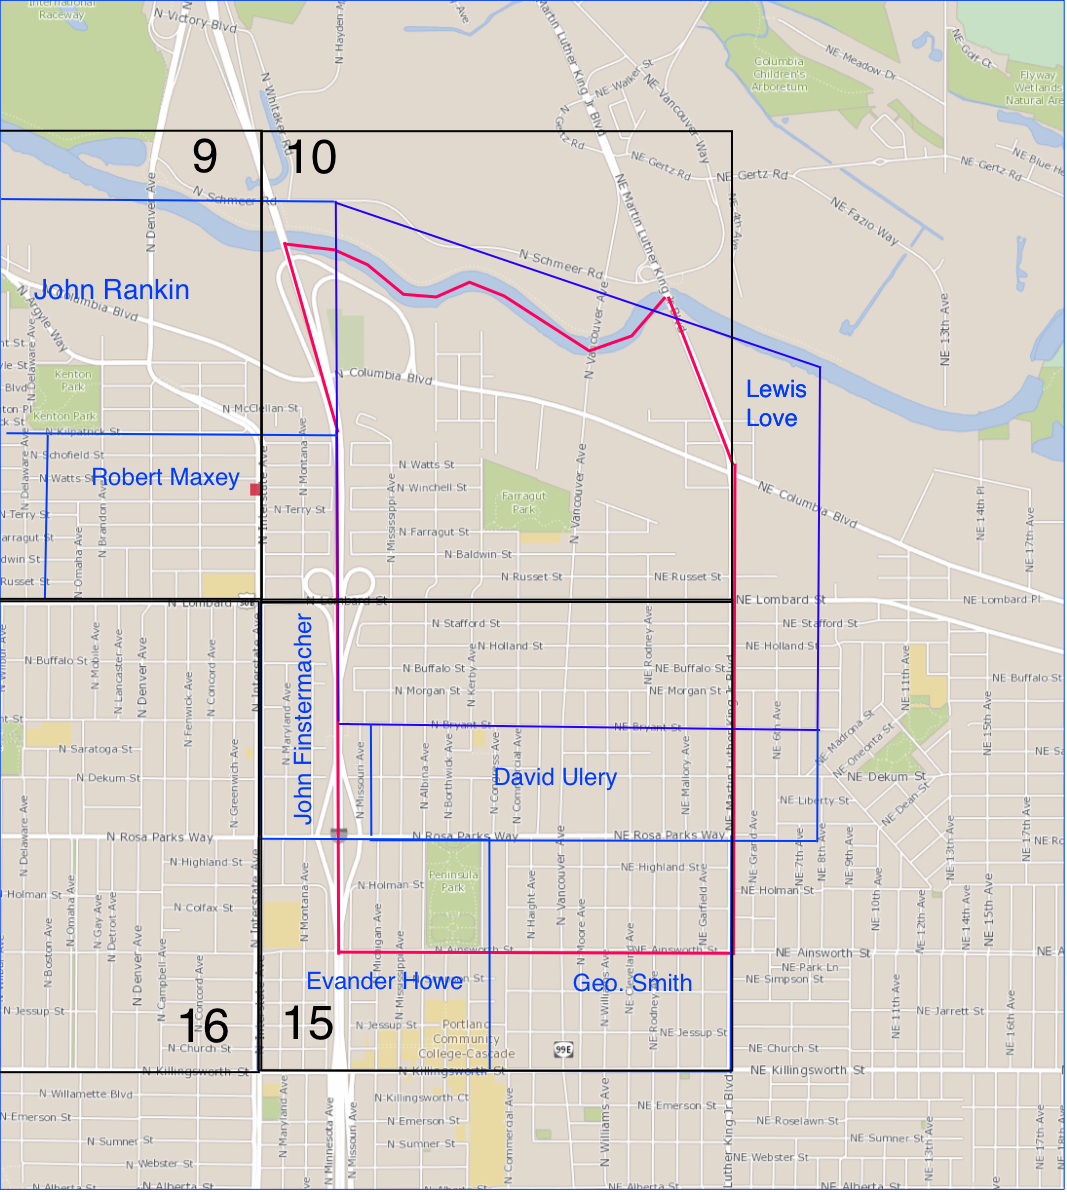
\includegraphics{images/02_images/image5.png}
\caption{alt\_text}
\end{figure}

\hypertarget{deeds-and-patents}{%
\subsection{Deeds and Patents}\label{deeds-and-patents}}

This book contains excerpts from, transcripts of, and links to hundreds of deeds. There are many types of deeds, which are used to register the transfer of real property. There are hundreds of introductions to deeds and types of ownership of real property of the web. A good example is \href{https://www.americanbar.org/newsletter/publications/law_trends_news_practice_area_e_newsletter_home/2011_summer/real_property_interests_deeds.html}{American Bar Association (2011)}. I only give a brief summary of the types we will encounter in this book.

A \emph{general warranty deed} guarantees that the grantor has clear title, and that no other parties retain an interest in the property. It usually includes various covenants, in particular that the grantor is responsible if it is discovered the title is not clear and third parties makes claims to the property.

A\_ quitclaim deed\_ transfers any interest in the real property that the grantee has to the grantor, without any guarantee that the grantee actually has title to or ownership of the property. Thus the rights of the grantor in the property are transferred to the grantee, provided that the grantor actually has these rights, otherwise the quitclaim deed is just a piece of paper.

A \emph{sheriff's deed} is a deed that gives ownership rights in property bought at a sheriff's sale. A sheriff's sale is a sale conducted by a sheriff upon order of a court after a failure to pay a judgment. These days sheriff's deeds are used in foreclosures, in the nineteenth century they were used even more often if owners of real property failed to pay taxes or bills for goods and services. The important thing is that a court order was needed. Old newspapers have pages and pages of pieces of real estate sold at sheriff's sales, mostly because of delinquent property taxes.

For US land donations and cash transactions under the homestead law we include and transcribe (in as far as they are readable) a copy of the patent and the corresponding deed. For later transfers of real property we include copies, or links to copies, of all deeds we could find. For this chapter we follow the title chain from the US to the homesteader, and then from the homesteader to all next-stage buyers, until the whole homestead is divided up and sold, and we arrive at the subdivision plats, which eventually all will have their separate chapters in this book.

As usual, links to deeds are included, and some deeds, or parts of deeds, are transcribed in the text. Because of the nineteenth century longhand, and because of the quality of the copies and microfilm, it is sometimes impossible to read part of the deed. Also, deeds are to a large extent written in legal language, portions of which are almost the same for all deeds in a certain period. In some cases we skip the boiler plate and only transcribe the variable portions. Finally, we do not transcribe the notarization of the deed, although that is typically included in the linked file.

\hypertarget{plats}{%
\subsection{Plats}\label{plats}}

\hypertarget{references-2}{%
\subsection{References}\label{references-2}}

Wikipedia: \emph{Public Land Survey System}

\url{https://en.wikipedia.org/wiki/Public_Land_Survey_System}

Wikipedia: \emph{Link (unit) }

\url{https://en.wikipedia.org/wiki/Link_(unit)}

Wikipedia: \emph{Rod (unit) }

\url{https://en.wikipedia.org/wiki/Rod_(unit)}

Wikipedia: \emph{Chain (unit) }

\url{https://en.wikipedia.org/wiki/Chain_(unit)}

Wikipedia: \emph{Furlong }

\url{https://en.wikipedia.org/wiki/Furlong}

Wikipedia: \emph{Donation Land Claim Act}

\url{https://en.wikipedia.org/wiki/Donation_Land_Claim_Act}

Wikipedia: \emph{Homestead Acts }

\url{https://en.wikipedia.org/wiki/Homestead_Acts}

American Bar Association (2011): \emph{Understanding Real Property Interests and Deeds. }\url{https://www.americanbar.org/newsletter/publications/law_trends_news_practice_area_e_newsletter_home/2011_summer/real_property_interests_deeds.html}

Champ Clark Vaughan (2014): \emph{A History of the United States General Land Office in Oregon.}

\url{https://www.blm.gov/or/landsrealty/glo200/files/glo-book.pdf}

Jerry A. O'Callaghan (1951): \_The Disposition of the Public Domain in Oregon. \_Doctoral Dissertation, Stanford. \url{https://drive.google.com/file/d/1T8HRj39qobQ_4NkydJpagwnRQvFPAEUB}

Roxanne Dunbar-Ortiz (2014): \emph{An Indigenous Peoples' History of the United States.}

Beacon Press, Boston, Massachusetts.

Eugene F. Snyder (1989): \emph{We Claimed this Land. Portland's Pioneer Settlers.}

Binfort \& Mort Publishing, Portland, Oregon

Lorenzo Veracini (2010): \emph{Settler Colonialism. A Theoretical Overview.}

Palgrave MacMillan, New York, NY

Walter L. Hixson (2013): \emph{American Settler Colonialism}

Palgrave MacMillan, New York, NY

J. Sakai (2014): \emph{Settlers. The Mythology of the White Proletariat from Mayflower to Modern.}

Kersplebedeb Publishing and Distribution, Montreal, Quebec

Morris Bien (1910): \emph{The Public Lands of the United States.} The North American Review, 192, 387-402 \href{https://drive.google.com/file/d/1TT_lgoh_nI8LSdztGw_claFQYfHje16G/view}{https://drive.google.com/file/d/1TT\_lgoh\_nI8LSdztGw\_claFQYfHje16G}

Genealogical Forum of Oregon (2014): Oregon Donation Land Claims. \url{https://drive.google.com/file/d/0B94Urj3OjM7BcWhIYmUtV0htcms}

Oregon History Project (2018): \emph{Oregon Land Donation Claim Notification}

\url{https://oregonhistoryproject.org/articles/historical-records/oregon-land-donation-claim-notification/\#.WriRZS-ZPDY}

\hypertarget{homesteads-evander-howe}{%
\section{Homesteads: Evander Howe}\label{homesteads-evander-howe}}

\begin{figure}
\centering
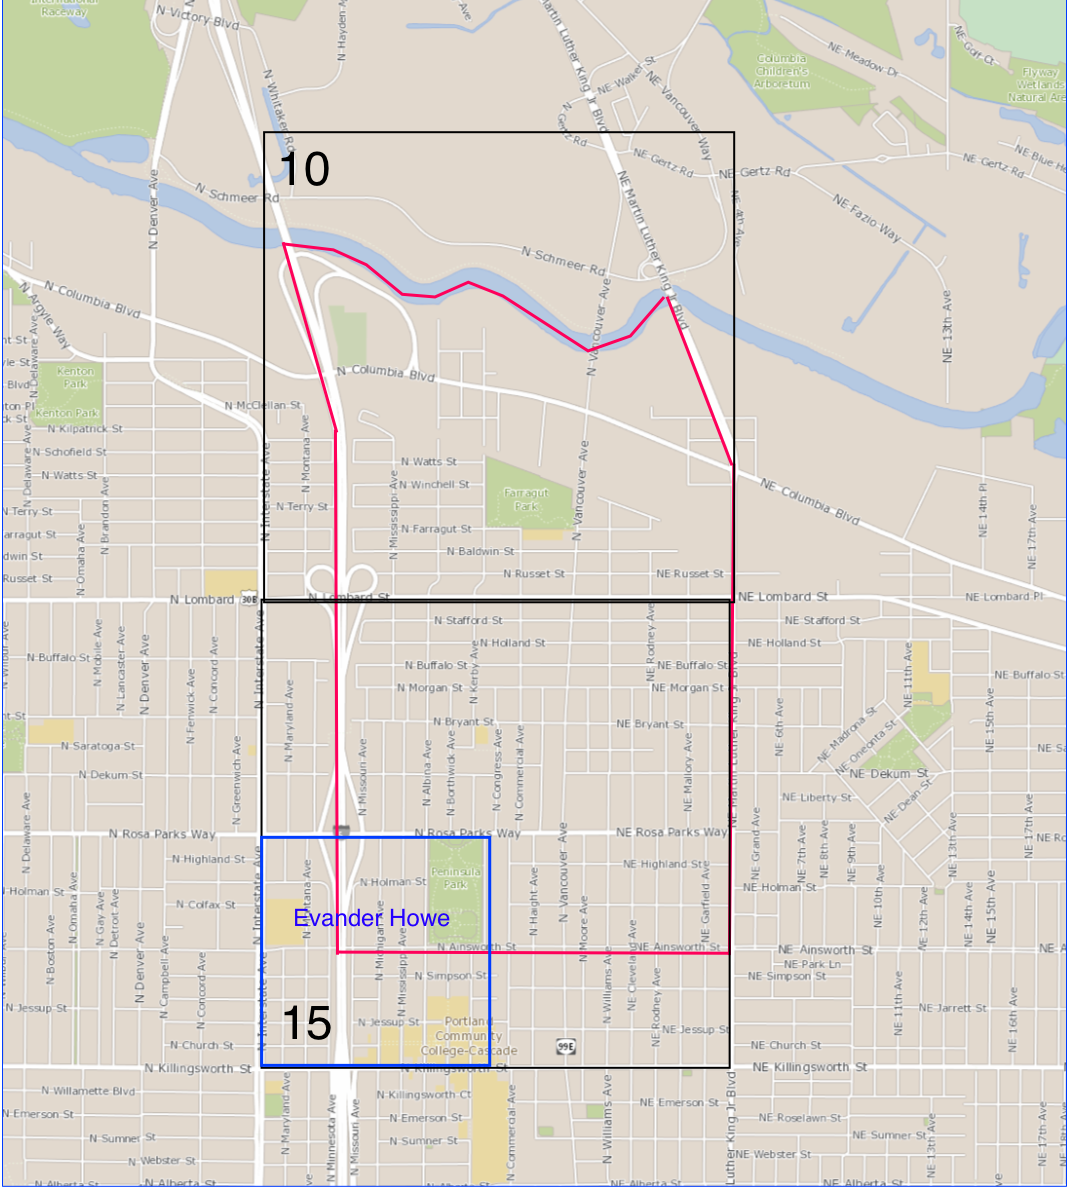
\includegraphics{images/0201a_images/image1.png}
\caption{alt\_text}
\end{figure}

\hypertarget{homestead}{%
\subsection{Homestead}\label{homestead}}

On June 1, 1870, Evander Howe established a claim under the homestead act of 1862 for 160 acres of land, the southwest corner of section 15 in township 1 north, range 1 east. Snyder tells us he paid \$ 200. That makes sense because under the provisions of the act land was sold for \$ 1.25 per acre. The complete transcribed text of the patent (General Land Office Record, 1870) follows.

\begin{quote}
Whereas there has been deposited in the General Land Office of the United States a certificate of the Register of the Land Office at Oregon City, whereby it appears that pursuing to the Act of Congress approved the 20th of May 1862 ``To Secure Homesteads to actual Settlers on the public domain'', and the acts supplemental thereto, the claim of Evander Howe has been established and duly consummated in conformity to law for the South West quarter of Section fifteen in Township one North of Range one East in this District of Lands subject to Sale at Oregon City Oregon containing one hundred and sixty acres according to the Official Plat of the Survey of the said Land returned to the General Land Office by the Surveyor General.
\end{quote}

\begin{quote}
Now know ye, that there is therefore granted by the United States onto the said Evander Howe the tract of land above described: the Have and To Hold the said tract of land with the appurtenances thereof unto the said Evander Howe and to his heirs and assigns forever.
\end{quote}

\begin{quote}
In testimony whereof I, Ulysses S. Grant, President of the United States of America, have caused these letters to be made Patent, and the Seal of the General and Office to be hereunto affixed.
\end{quote}

\begin{quote}
Given under my hand, at the City of Washington, the first day of June, in the year of our Lord one thousand eight hundred and seventy, and of the Independence of the United States the ninety fourth.
\end{quote}

\begin{quote}
By the president (signed) U.S. Grant, by (signed) Charles White, Sec'y, (signed) J.N. Granger, Recorder of the General Land Office.
\end{quote}

\url{https://drive.google.com/file/d/0B94Urj3OjM7Bd0RkakpYTktEc2s}

To show where Evander Howe's homestead was located, I have included a map at the beginning of this section/ In the map sections 10 and 15 in township 1 north, range 1 east are drawn in black. The blue Evander Howe square, half a mile by half a mile, in the southwest corner is bounded by what is now Interstate Avenue, Kerby Avenue, Killingsworth Street, and Rosa Parks Way. Parts are in modern Piedmont (within the red boundaries), parts are in Humboldt, Overlook, and Arbor Lodge.

\hypertarget{sales}{%
\subsection{Sales}\label{sales}}

Evander Howe sold eighty acres on July, 5 1870 for four hundred dollars to Elizabeth Smith, who, together with her husband George Smith, owned the 160 acres to the east since March 10, 1866. The eighty acres Evander sold to the Smiths were the lower half of the blue quadrant, i.e.~the part in modern Humboldt and Overlook.

\begin{quote}
Know all men by these Presents: That I Evander Howe in consideration of four Hundred Dollars to me paid by Elizabeth Smith do hereby bargain, sell, and convey to said Elizabeth Smith her heirs and assigns forever the following described parcel of real estate to wit: the South half of West Quarter of Section fifteen in Township one North range one East and bounded as follows. Commencing at the South West corner of Section fifteen and running North eighty rods thence running east one hundred and sixty rods thence South eighty rods thence West one hundred and sixty rods to place of beginning containing eighty acres said property is located in the County of Multnomah State of Oregon. \_
\end{quote}

\begin{quote}
To Have and To Hold the same with all the privileges and appurtenances belonging to the said Elizabeth Smith her heirs and assigns forever. And I do covenant with the said Elizabeth Smith and her legal representatives forever, that the said premises are free from all encumbrance and that I will and my heirs, executors and administrators shall Warrant and Defend the same to the said Elizabeth Smith her heirs and assigns forever, against the lawful claims and demands of all persons whatsoever. In Witness Whereof I have hereto set my hand and seal this fifth day of July A.D. 1870.\_
\end{quote}

\begin{verbatim}
_[https://drive.google.com/file/d/1PiJlcxtVmqaULLe7XHCWsoMWEnVwgHo5/view](https://drive.google.com/file/d/1PiJlcxtVmqaULLe7XHCWsoMWEnVwgHo5/view)_
\end{verbatim}

Evander Howe did not sell the other half in his lifetime. Or, to be more precise, he sold it for forty dollars on July 12, 1870 to John Hotts, his neighbor, a retired farmer on the Columbia, who went into real estate transactions later in life. And then he bought it back from Hotts for one hundred dollars on November 5 of that year. Here is the text of the deeds. First from Howe to Hotts.

\begin{quote}
Know all men by these Presents: That I Evander Howe of Multnomah County Ogn in consideration of Forty Dollars to me paid by John Hotts of same place. Do hereby bargain, sell, and convey to said John Hotts his heirs and assigns forever the following described parcel of real estate to wit: the North half of the South west Quarter of Section fifteen (15) in Township One North Range One East containing eighty acres in Multnomah County State of Oregon.
\end{quote}

\begin{quote}
To Have and to hold the same with all the privileges and appurtenances thereto belonging to the said John Hotts his heirs and assigns forever. And I do covenant with the said John Hotts and his legal representatives forever, that the said premises are free from all encumbrance and that I will and my heirs, executors and administrators shall Warrant and Defend the same to the said John Hotts his heirs and assigns forever, against the lawful claims and demands of all persons whatsoever. In Witness Whereof I have hereto set my hand and seal this Twelfth day of July A.D. 1870. (signed) Evander Howe\_
\end{quote}

\begin{verbatim}
_[https://drive.google.com/file/d/1PyOtjEaGyvoSKLLvfJP47aOp6nn6BtqY/view](https://drive.google.com/file/d/1PyOtjEaGyvoSKLLvfJP47aOp6nn6BtqY/view)_
\end{verbatim}

Then from Hotts to Howe.

\begin{quote}
Know all men by these Presents:** **That I John Hotts of Multnomah County Oregon in consideration of One Hundred Dollars to me paid by Evander Howe do hereby bargain, sell, and convey to said Evander Howe his heirs and assigns forever the following described parcel of real estate to wit: the North half of the South west Quarter of Section fifteen (15) in Township One North Range One East containing eighty acres in Multnomah County Oregon.
\end{quote}

\begin{quote}
To Have and to hold the same with all the privileges and appurtenances thereto belonging to the said Evander Howe his heirs and assigns forever. And I do covenant with the said Evander Howe and his legal representatives forever, that the said premises are free from all encumbrance and that I will and my heirs, executors and administrators shall Warrant and Defend the same to the said Evander Howe his heirs and assigns forever, against the lawful claims and demands of all persons whatsoever. In Witness Whereof I have hereto set my hand and seal this 5 day of November A.D. 1870. (signed) John Hotts
\end{quote}

\begin{verbatim}
_[https://drive.google.com/file/d/1Q1bc6cNj1x-ssB3AXnrFnUO2-VMFzShy/view](https://drive.google.com/file/d/1Q1bc6cNj1x-ssB3AXnrFnUO2-VMFzShy/view)_
\end{verbatim}

Evander Howe died childless, a lifelong bachelor. In the \emph{Vermont Watchman and State Journal} of January 17, 1883, we see the following announcement.

\begin{figure}
\centering
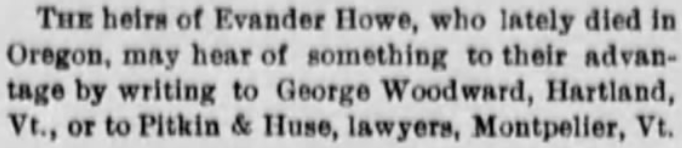
\includegraphics{images/0201a_images/image2.png}
\caption{alt\_text}
\end{figure}

As a direct result of this there are three deeds, all dated February 5, 1883, in which the heirs of Evander Howe deed the northern 80 acres to George Woodward of Portland, for the total sum of \$ 8000. It looks like George Woodward traveled east to find these heirs. The text of the deeds Is given below. The first one, signed by Hannibal and Maria Howe, is

\begin{quote}
Know all men by these presents, that we Hannibal F. Howe, a brother of Evander Howe late of Multnomah County Oregon deceased, and Maria M. Howe, wife of said Hannibal F. Howe, both of Jamaica in the County of Windham and State of Vermont, in consideration of the sum of Two Thousand Dollars to us paid by George Woodward of the City of Portland in the County of Multnomah in the State of Oregon, the receipt of which we hereby acknowledge, do hereby convey, remise, release and forever quitclaim unto the said George Woodward his heirs and assigns all that tract or parcel of land situated in said County of Multnomah in said State of Oregon described as follows: viz: All of the north half of the south west of section numbered fifteen (15) in Township numbered One (1) north of Range One (1) east of the Willamette Meridian containing eighty acres more or less; meaning to convey all the land that the said Evander Howe deceased was possessed of at the time of his decease in said Section fifteen (15) Township One (1) north Range One (1) east, with all the privileges and appurtenances thereunto belonging.
\end{quote}

\begin{quote}
To Have and To Hold the above granted and bargained premises to the said George Woodward his heirs and assigns, to his and their use benefit and behoof forever. And me the said Hannibal F. Howe and Maria M. Howe for ourselves our heirs executors and administrators do covenant with the said George Woodward his heirs and assigns hat the premises are free from all encumbrances made or suffered by us, and that we will, and our heirs, executors, and administrators shall warrant and defend the same to the said George Woodward his heirs and assigns forever against lawful claims of all persons claiming by, through, or under us, but against none other. In witness whereof we have hereunto set our hands and seals this 5th day of February AD 1883. (signed) Hannibal F. Howe (signed) Maria M. Howe
\end{quote}

\begin{verbatim}
_[https://drive.google.com/open?id=1rpuDpZYpYVq0iQlaqPtUDrRAraEY5gk7](https://drive.google.com/open?id=1rpuDpZYpYVq0iQlaqPtUDrRAraEY5gk7)_
\end{verbatim}

The second one, signed by Ezra and Etta Howe, is identical, except for the different names of the grantors, and the fact that they lived in Brattleboro, County of Windham. The first two deeds were notarized in Vermont.

\url{https://drive.google.com/open?id=1wxfhNyWLkp815Ko7rQcvGhNBFBzQWCwW}

The third deed, notarized in Connecticut, starts with

\begin{quote}
Know all men by these presents, that we Lovina A. Sweet, a sister of Evander Howe late of Multnomah County, Oregon, deceased and Edward H. Sweet, husband of said Lovina H., and Sarah L. Yance, a sister of said Evander Howe, deceased, and Lorenzo Yance, husband of said Sarah L., all of Meriden, in the County of New Haven, in the State of Connecticut, in consideration of the sum of Four Thousand Dollars \ldots\_
\end{quote}

\url{https://drive.google.com/open?id=1CZDyWK0AwXhS4wodoqFr5P4mZ8O4tltb}

Eugene Snyder (1989, p.~114) says a brother Estey Howe from Battleboro, Vermont, inherited the whole 80 acres, worth \$ 6000, but that is incorrect. There is no Estey Howe, I think. Also, there is no Battleboro in Vermont, although there is a Brattleboro. Snyder was misinformed by the \href{https://drive.google.com/open?id=1xs6X_Qrkn7oQ42qUxIBs0PgluGlfWPlM}{Evander Howe probate file}, which mentions one Estey Howe as a possible sole heir. As we have seen, that should be Ezra Howe, and there were others.

On December 27, 1883 George Woodward and Ellen M. Woodward, his wife, quitclaimed for one dollar an undivided one-third interest in the northern 80 acres to assembly and councilman Sylvester Farrell, of Everding \& Farrell, a huge wholesale produce, shopping, grain, salmon, and logging company. And on the same day they also transferred another undivided one-third interest in the northern half of the southwest quarter to local undertaker and capitalist Edward Holman for another dollar.

\url{https://drive.google.com/open?id=1uheS9b7nigCNVkVcf4-3Ve6vU0F7mASU}

\url{https://drive.google.com/open?id=1_inDXj_kQkbhkHclvA2Fw-oLh-jv_QzC}

August 17, 1887 a one-third interest was transferred from Farrell to Everding \& Farrell for \$ 2,500.

\url{https://drive.google.com/open?id=1LqahDe7DqF0VmlcNryMhDq1OUgd9WXNK}

On January 3, 1890 S. Farrell and Edward Holman sold their undivided two-thirds interest to W. K. Smith for \$ 26,666.66.

\url{https://drive.google.com/open?id=16X24Gs1i2tG0iPP8j7WRHGVSS9nJcluZ}

Finally, on January 16, 1918 Everding \& Farrell sold their one third interest to the Ukase Investment Co for the nominal sum of \$ 1.

\url{https://drive.google.com/open?id=1kkzW2tZrt2BnMOHI0Hi8BiZWxaxC2PnS}

From 1918 on the Ukase Investment Company controlled the complete 80 acres in the northern half of the south west quadrant of section 15. The land had increased in value from
\$ 100 in 1870 to \$ 40,000 in 1890. Of course very little of that appreciation benefited Evander Howe, although some of it benefited his heirs in Vermont.

In other places in this book I will discuss what the Ukase Investment Company did with their 80 acres. They leased some of the land to Harry Bush for Evergreen Park and to the City for the Municipal Automobile Park. They sold some of the land to the school district for Ockley Green School and to the City for Peninsula Park. And they used 25 of the 80 acres to plat and develop the Gainsborough Addition.

As we have seen the southern half of Evander Howe's quadrant was not in Piedmont. The eastern part of this southern half became West Piedmont and Jarrett's Addition, the western part became North Albina.

\hypertarget{homesteaders-evander-howe}{%
\section{Homesteaders: Evander Howe}\label{homesteaders-evander-howe}}

\hypertarget{life}{%
\subsection{Life}\label{life}}

In the 1860s Evander Howe came from Vermont to Oregon. He does not appear even once in any of the Oregon newspapers from the time period. Eugene E. Snyder \_(1989, p.~114) \_says

\begin{quote}
\emph{No record tells us what sort of man Evander Howe was, nor how he occupied his time in Oregon.}
\end{quote}

As I began this research it was unclear when and where he was born and how old he was when he died. There is not much information, but there is a bit more than nothing.

Snyder mentions he has no idea what Howe tried or did during his final years, or if he was even in Portland. But I found him in the 1880 census. He was enumerated on July 14, a 45 year old farmer living in the Willamette Precinct. The name was transcribed as Evanden, but the census form is pretty clear. His neighbor on the form is the 52 year old farmer John Hott (sic). That should actually be John Hotts. Both of them were single. Evander apparently lived alone, Hotts had a hired hand living at the same address. Another neighbor on the same census form is Davis Ulery (sic), a 49 year old farmer, with a large family. That should actually be David Ulery.

\url{https://drive.google.com/file/d/1UG_QRBABD8gPf79ShC7yWP__qr3oubIK/view}

\hypertarget{death}{%
\subsection{Death}\label{death}}

Snyder tells us Evander Howe died in 1882. Initially, I was not able to find the precise date of death, or the location of the grave. But there is much useful information, as is often the case, in the probate file (Case number 858, Multnomah Court Records, 56 pages).

\url{https://drive.google.com/open?id=1xs6X_Qrkn7oQ42qUxIBs0PgluGlfWPlM}

As I have remarked elsewhere, probate files and cemetery records often make it easier to find out facts about a person's death than about their life. This is partly because they arrived from different places, but they all died in Portland. Also, their birth and childhood often were lived in areas that were not yet incorporated and did not have state, county, or city administrative offices. And thirdly, there is just more bureaucratic and journalistic activity around estates and deaths than around births or marriages, partly because often the heirs tend to get into elaborate fights amongst themselves. This is, of course, especially true for large estates, because greed needs a substrate to grow on.

So what did I learn from the probate file ? Evander Howe died intestate on June 24, 1882. Thus the court had to appoint an administrator to oversee the appraisal and distribution of the estate. In order to get the job potential administrators petition the court for an appointment, usually pointing out why they were especially suited for the position. In Howe's case there were two petitioners. The first was R. G. Rex M.D.~who was ``one of the principal creditors of said deceased''. Also Dr.~Rex had some pertinent information. In his petition he gave the precise description of Evander's real estate, and its estimated value of \$ 8,000, and he knew of the existence of `` a brother names Estey Howe residing at or near Brattleboro in Windham County in the State of Vermont.'' Nevertheless Dr.~Rex lost out to Edward Holman, the funeral and cremation provider, who ran ``the second oldest business in Portland'', since 1854. The business still exists. See their website at \url{https://www.holmansfuneralservice.com}. There was a great deal of money in funerals, it seems, and Holman became a capitalist, and a very prominent citizen of Portland. Note that soon after he would actually own a half interest in Evander's land.I don't think Dr.~Rex stood a chance, even though he knew the deceased and Holman did not.

In his petition Holman mentioned that Evander Howe had no family in Oregon, or anywhere else, as far as he knew. But he did mention he was the principal creditor of the estate. The firm of A.P. De Lin \& Co, of which he was a member, was owned \$ 128.00 for funeral services. The bill in question is below. It does not say where the grave was, and I still do not know where A.P. De Lin \& Co.~generally disposed of the bodies.

\begin{figure}
\centering
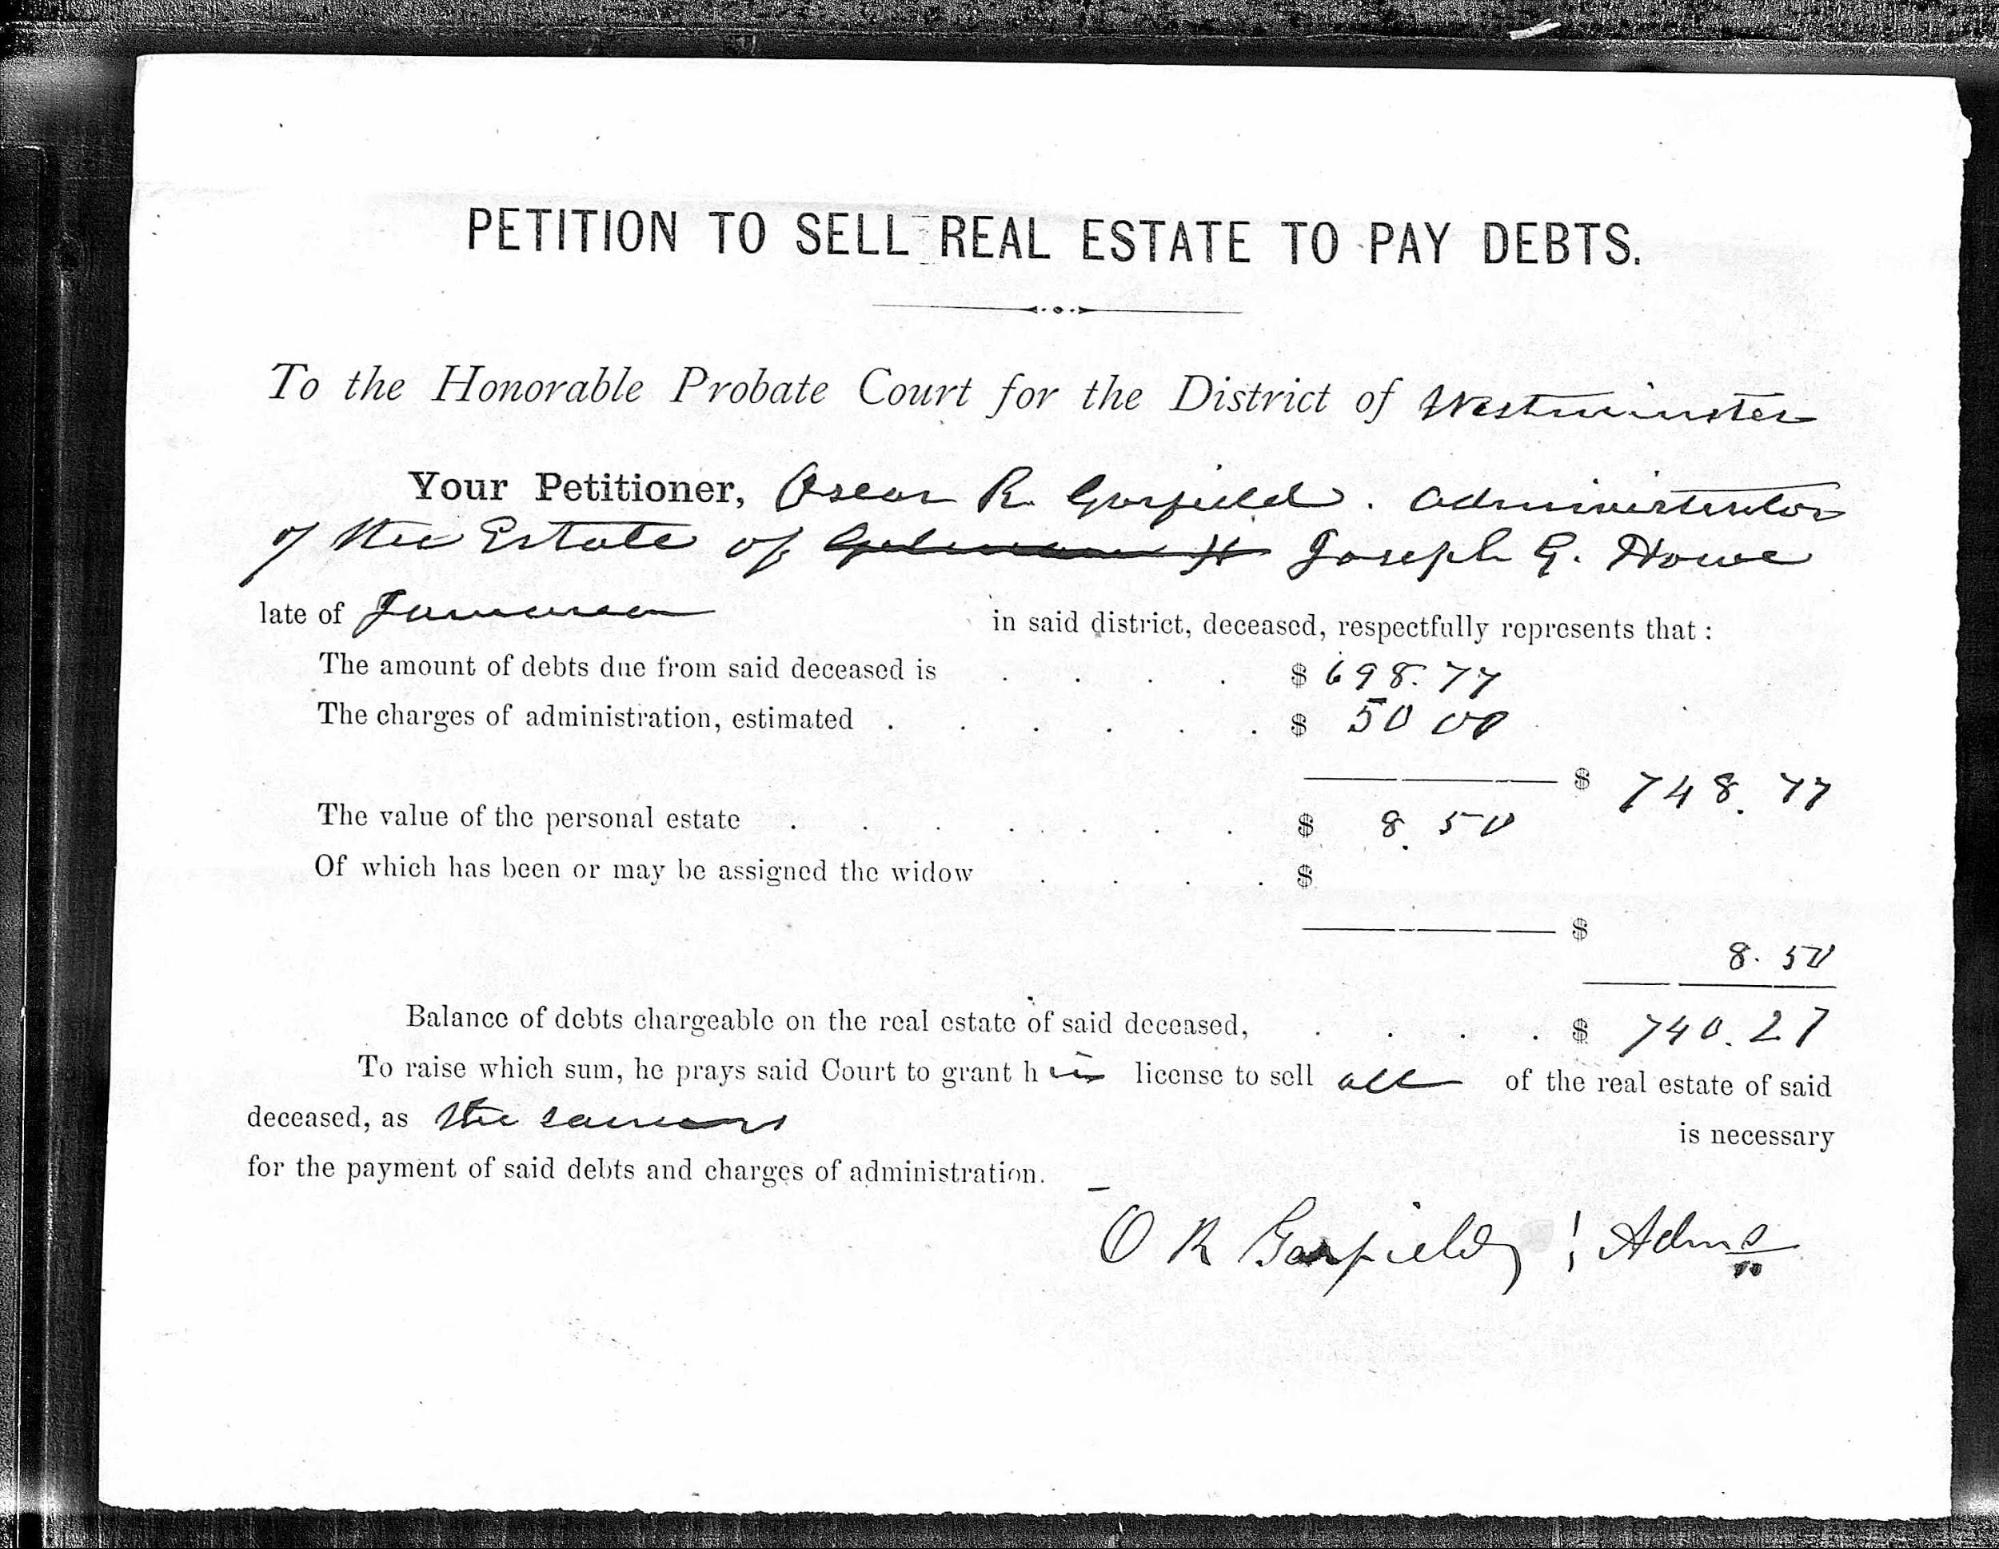
\includegraphics{images/0201b_images/image1.jpg}
\caption{alt\_text}
\end{figure}

Being an administrator required one to agree to a financial penalty if the court found the duties of the administrator were not carried out or the powers of the administrator were misused. In the Evander Howe case Holman had to agree to a penal sum of \$ 12,000. He used two sureties, Levi Anderson and councilman Sylvester Farrell, each for \$ 6,000. Note again that soon after Sylvester Farrell would own a half interest in Evander's land.

The appraisers were D.W. Wakefield, L.L. Parrish, and T.J. Mattock. They concluded, probably without actually looking at anything, on August 11, 1882 that there was \$ 200.00 of cash and \$ 8,500.00 of real property (the northern half of the southwest quarter of section 15). In his final report, of August 24, 1882, Holman adds \$ 12.45 from the sale of potatoes (which were a common part of agricultural estates) and \$ 28.62 from the sale of an old stove and some other personal property. He paid some outstanding bills and charged additional costs to the estate, including a \$ 150.00 appraiser fee for himself and a \$ 100.00 fee for his lawyer. Here is the list.

Clearly Evander Howe lived a minimalist and environmentally responsible life on his piece of the Vancouver Road.

\begin{figure}
\centering
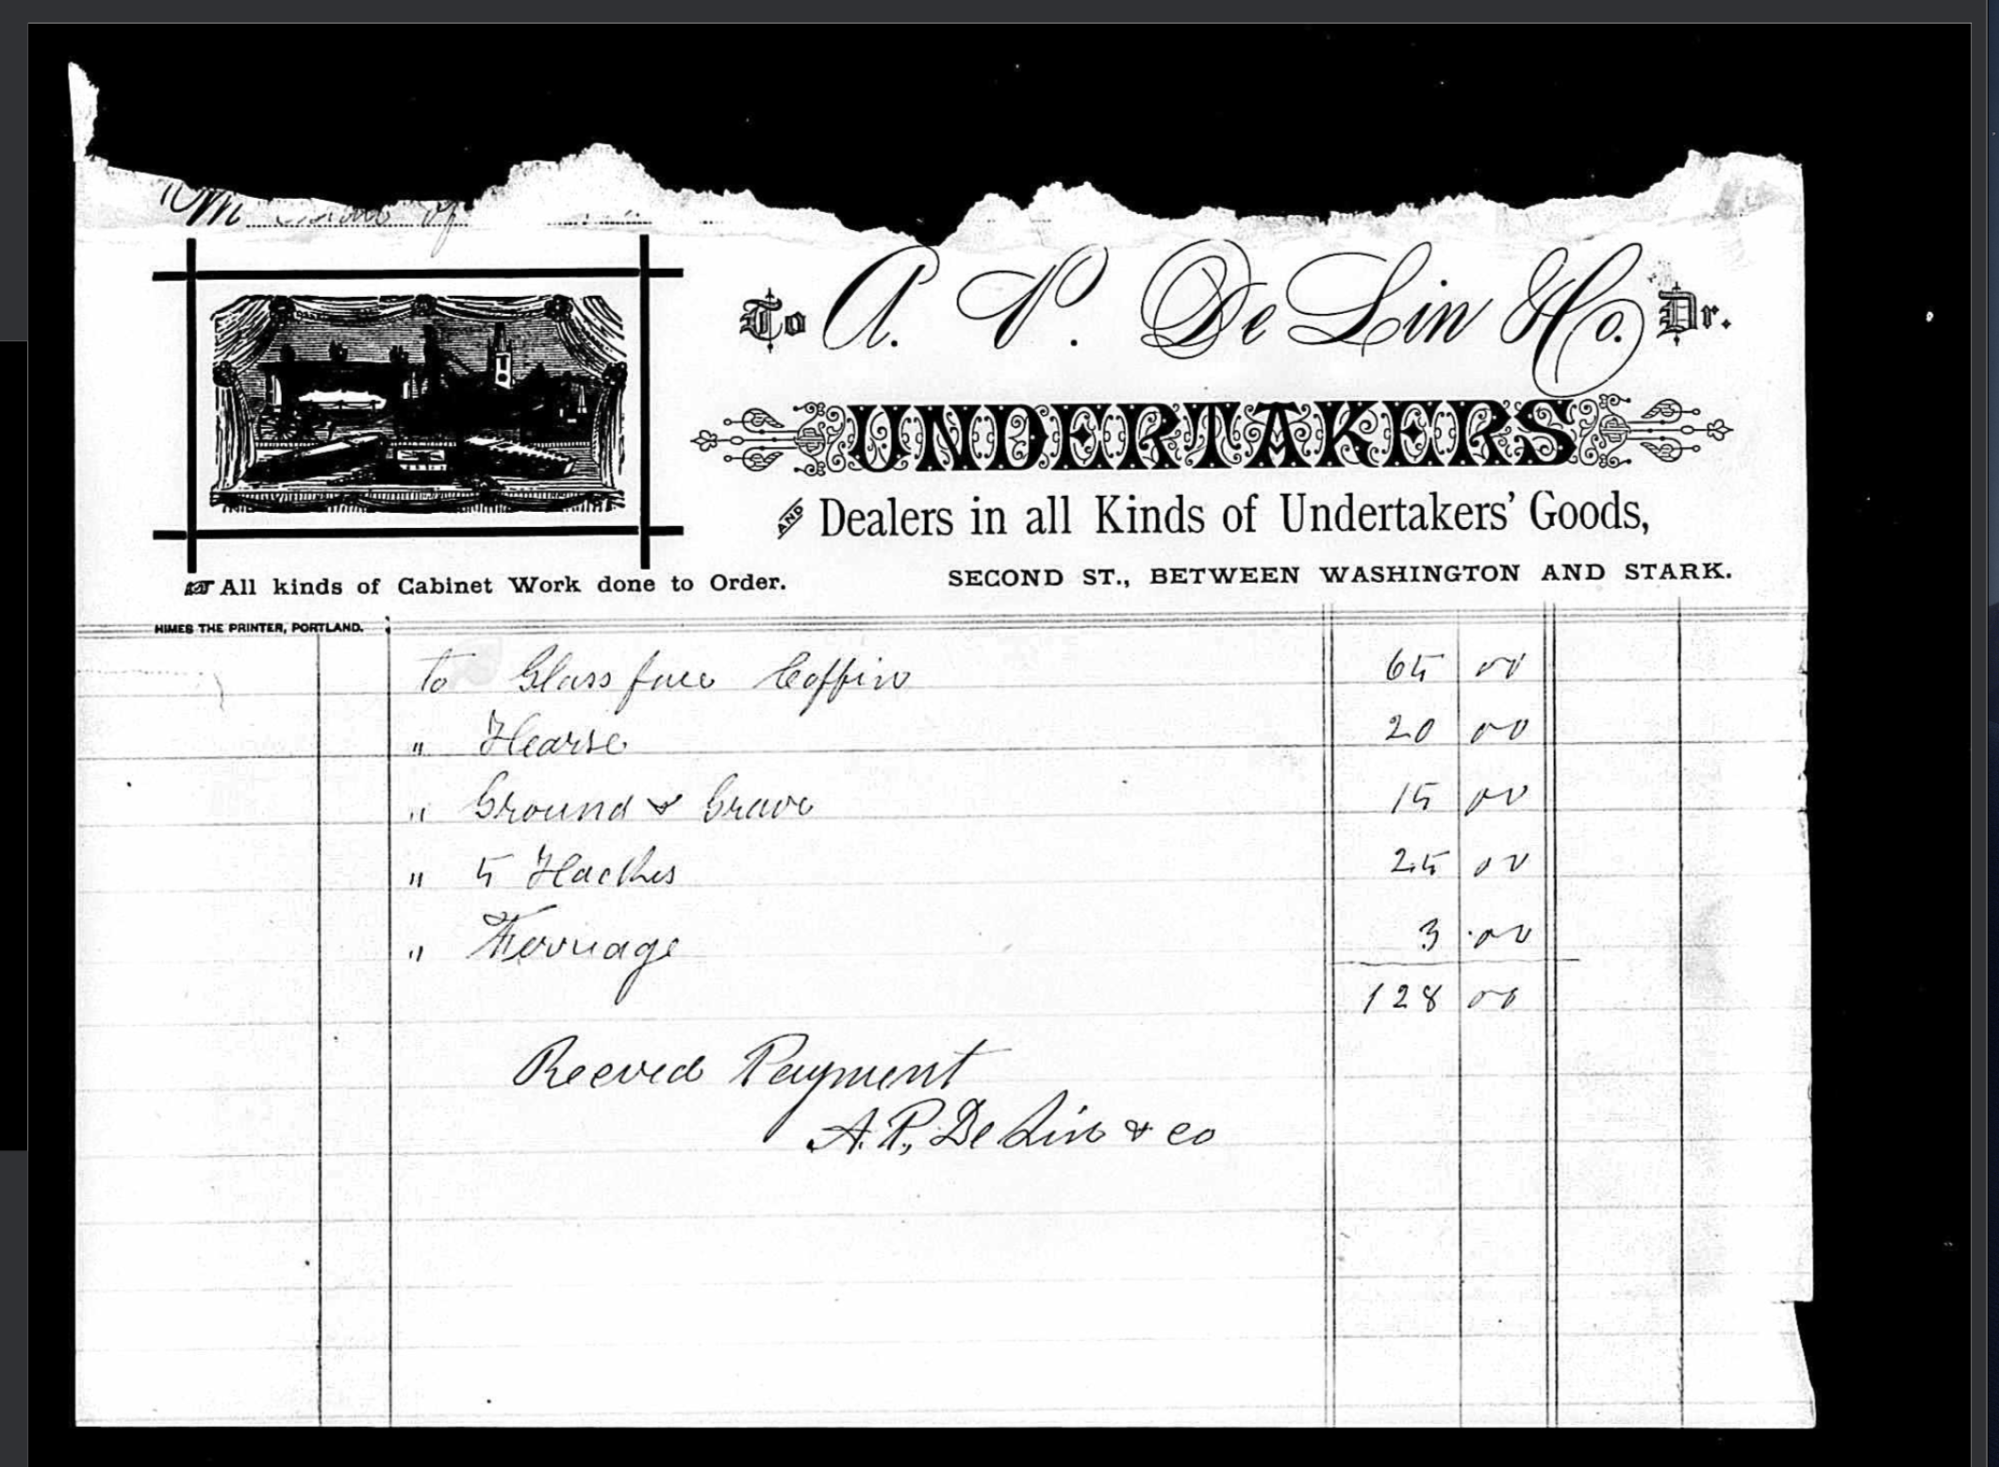
\includegraphics{images/0201b_images/image2.png}
\caption{alt\_text}
\end{figure}

What follows in the probate file are copies of the bills, and various notices from the creditors that the bills were duly paid. More interesting for our purposes is a later note, notarized on March 22, 1883, and written by Edward Holman's attorney to Judge Stearns. It shows that George Woodward, perhaps taking a hint from the petition of Dr.~Rex, had found the family.

Edward Holman, Sylvester Farrell, and W. K. Smith were waiting in the wings to start buying and selling the land.

\begin{figure}
\centering
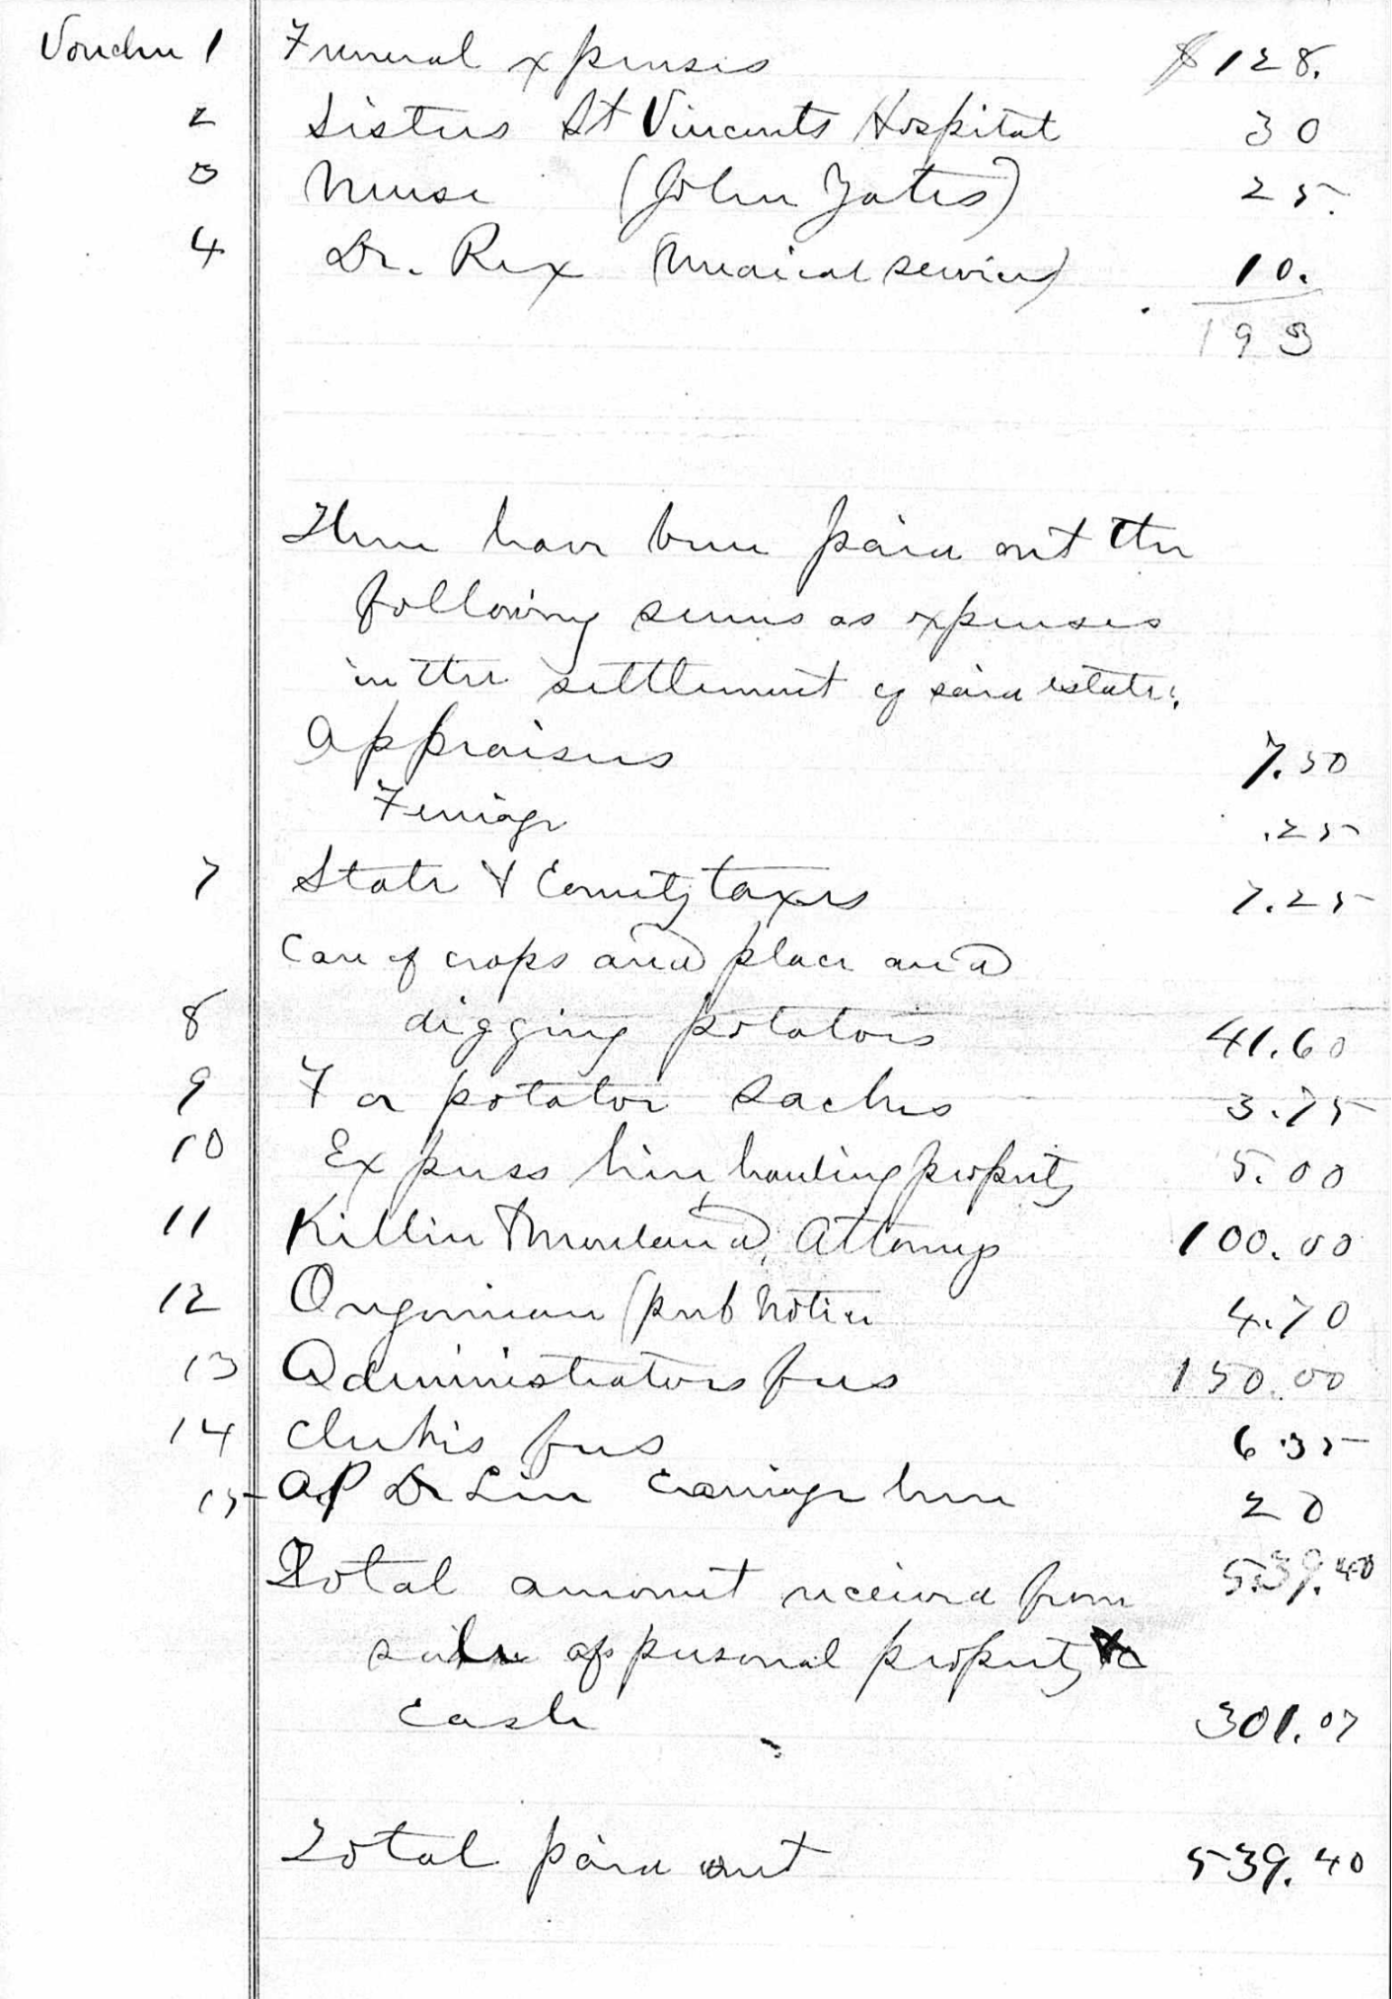
\includegraphics{images/0201b_images/image3.png}
\caption{alt\_text}
\end{figure}

\hypertarget{family}{%
\subsection{Family}\label{family}}

We have seen earlier that Evander's family lived in Vermont. In the 1850 \emph{Federal Census} I found Joseph Gilman Howe, a farmer, born 1809, married to Priscilla Howe (née Spalding) and living in Jamaica, Windham County, Vermont. They have five children living at home: Evander, age 15, Hannibal, age 12, Louisa, age 10, Lovina, age 7, and Sarah, age 4. Thus Evander was the oldest son. The \emph{Vermont Vital Records} show his birth date was March 12, 1834. It also shows the middle initial T. which disappeared over time.

\begin{figure}
\centering
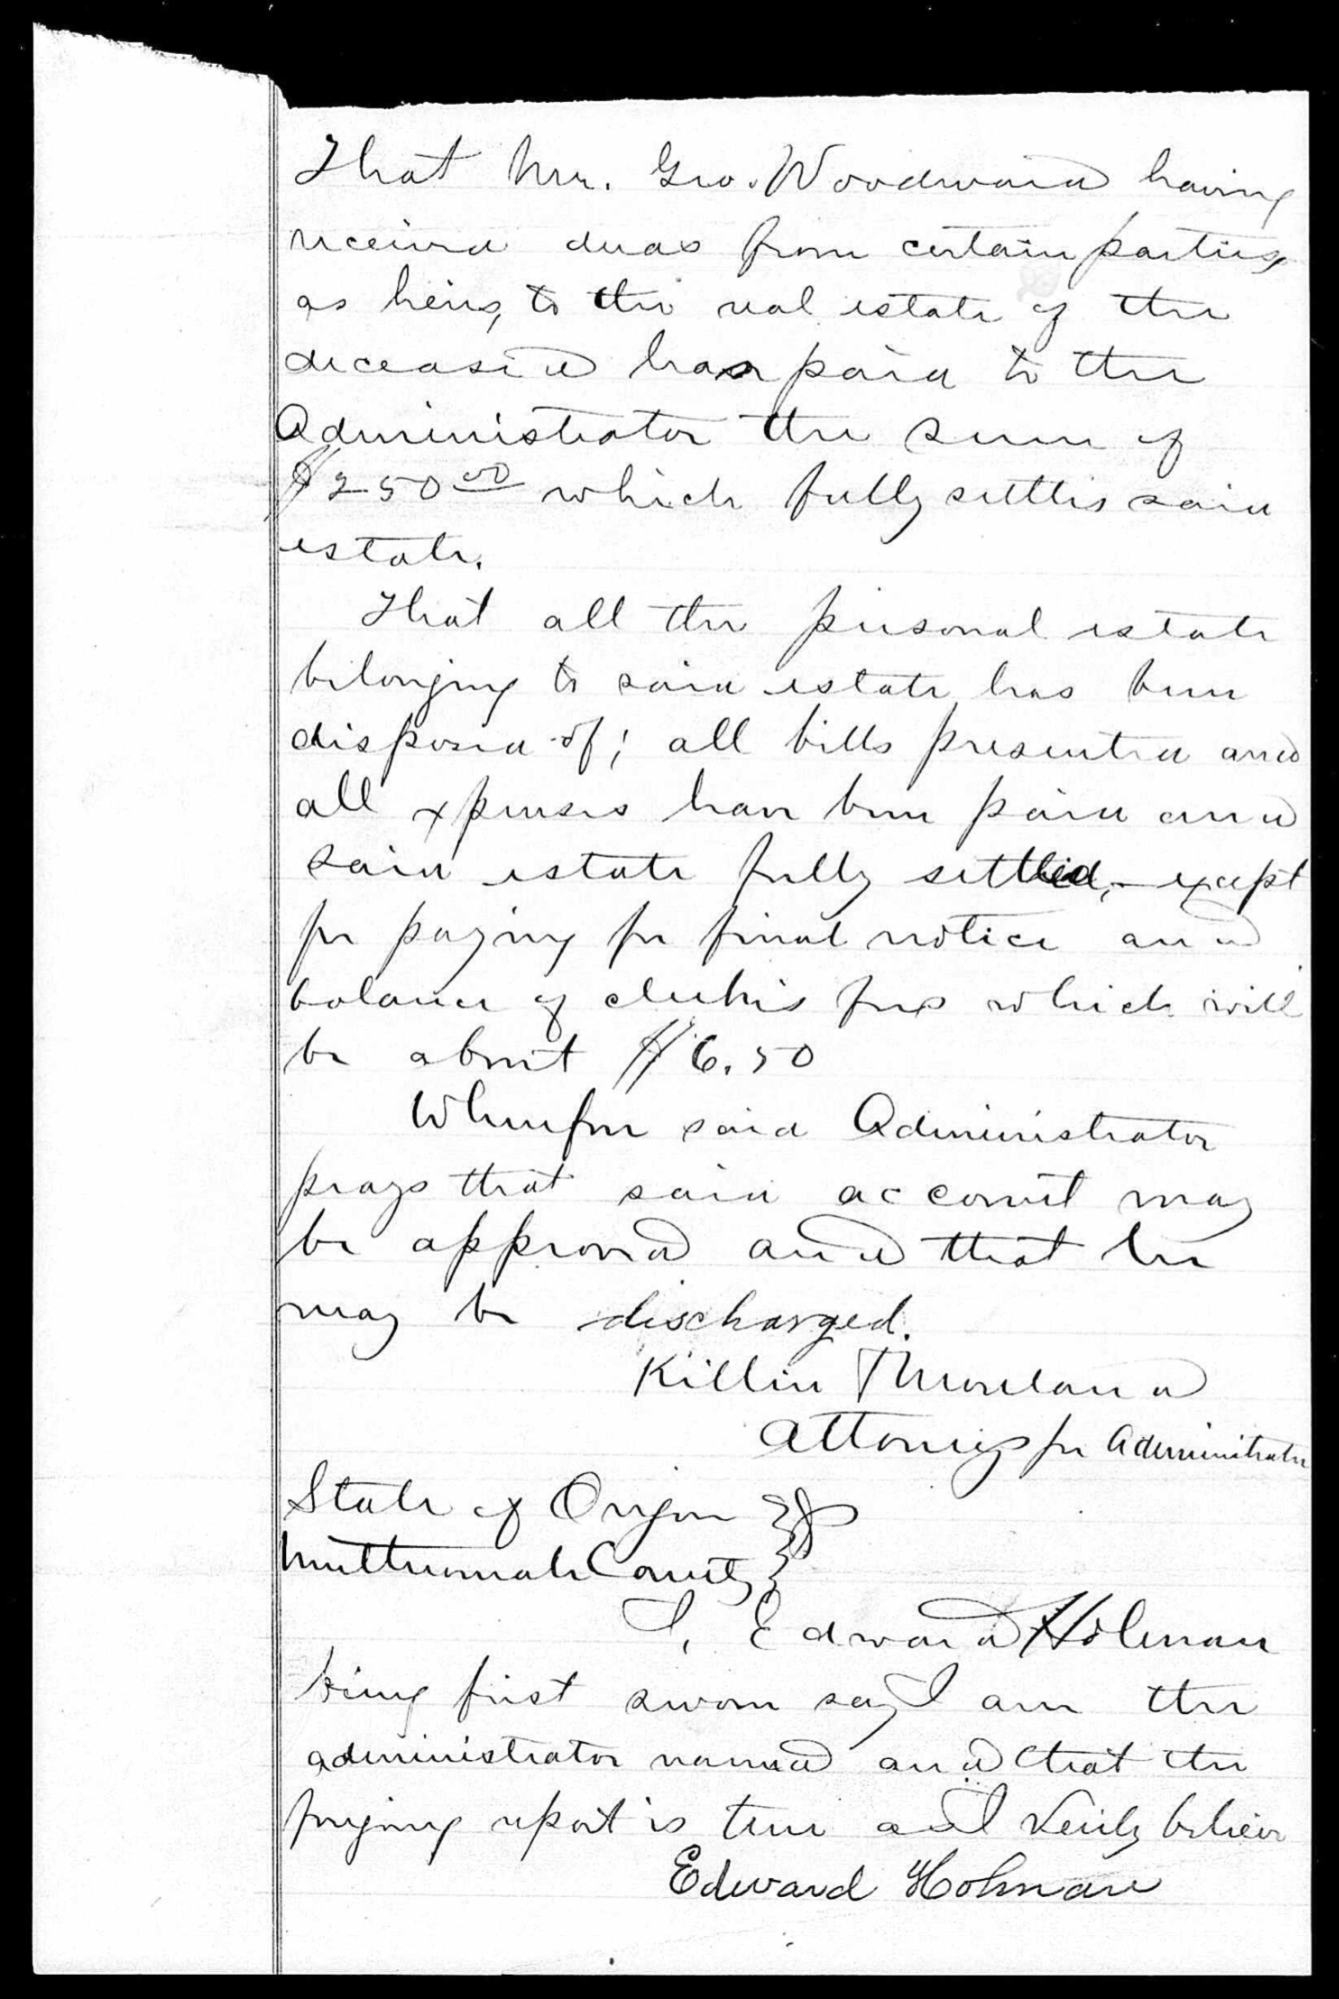
\includegraphics{images/0201b_images/image4.png}
\caption{alt\_text}
\end{figure}

\url{https://drive.google.com/file/d/0B94Urj3OjM7BeldUckFKSUx0blk/view}

Evander's profession at 15 was listed by the census as farmer, like his dad. In the 1860 census Evander (transcribed as Elander) was 24, still living at home, a laborer. There is now also an eight year old brother Ezra Olander Howe.

I also found a record in the \emph{Minnesota Territorial Census} of September 21, 1857, showing an Evander Howe, age 23, born in Vermont in 1834, living in Township 109 in the County of Nicollet. He was a laborer on the farm of Luke Rist, who was also from Vermont. And in the \emph{Minnesota Homestead and Cash Entry Patents} Evander Howe bought 27.62 acres of land in Blue Earth, Nicollet County, on October 1, 1860. The land office that handled the sale was in St Peter, another town in Nicollet County. Even more impressively, on December 3, 1860, Sarah Knecht, formerly the widow of Henry Stone, who was a private in Captain Wilson's Company of the Pennsylvania Militia in the War of 1812, used the Military Bounty Act of 1855 to claim 120 acres of land in Nicollet County. She then assigned the warrant to H.W. Lamberton, who subsequently passed it on to Evander Howe. So clearly around this time Evander was moving west and had acquired some property on the way. I have copies of both patent deeds, but since they are a bit far from our bed, and transcribing them is boring, I will just give the URLs in the references. I have no idea what Evander did between 1860 and 1870.

In the 1880 census Joseph G. Howe is a widower, who lives with his daughter-in-law Maria and two grandchildren, still in Jamaica, Vermont. There is no sign of Hannibal, Maria's husband. It is mentioned in the census that Joseph is sick of old age. He died 1882, 74 years old, in the same year as his oldest son Evander. The \emph{Vermont Probate Records} of 1882 show that the administrator of his estate asks permission of the probate court to sell all real estate belonging to the deceased to satisfy his debtors. There is a debt of \$ 698.77 and a personal estate of only \$ 8.50. The 8000 dollars that Geo. Woodward paid to Evander Howe's siblings came too late to help Joseph Howe.

\begin{figure}
\centering
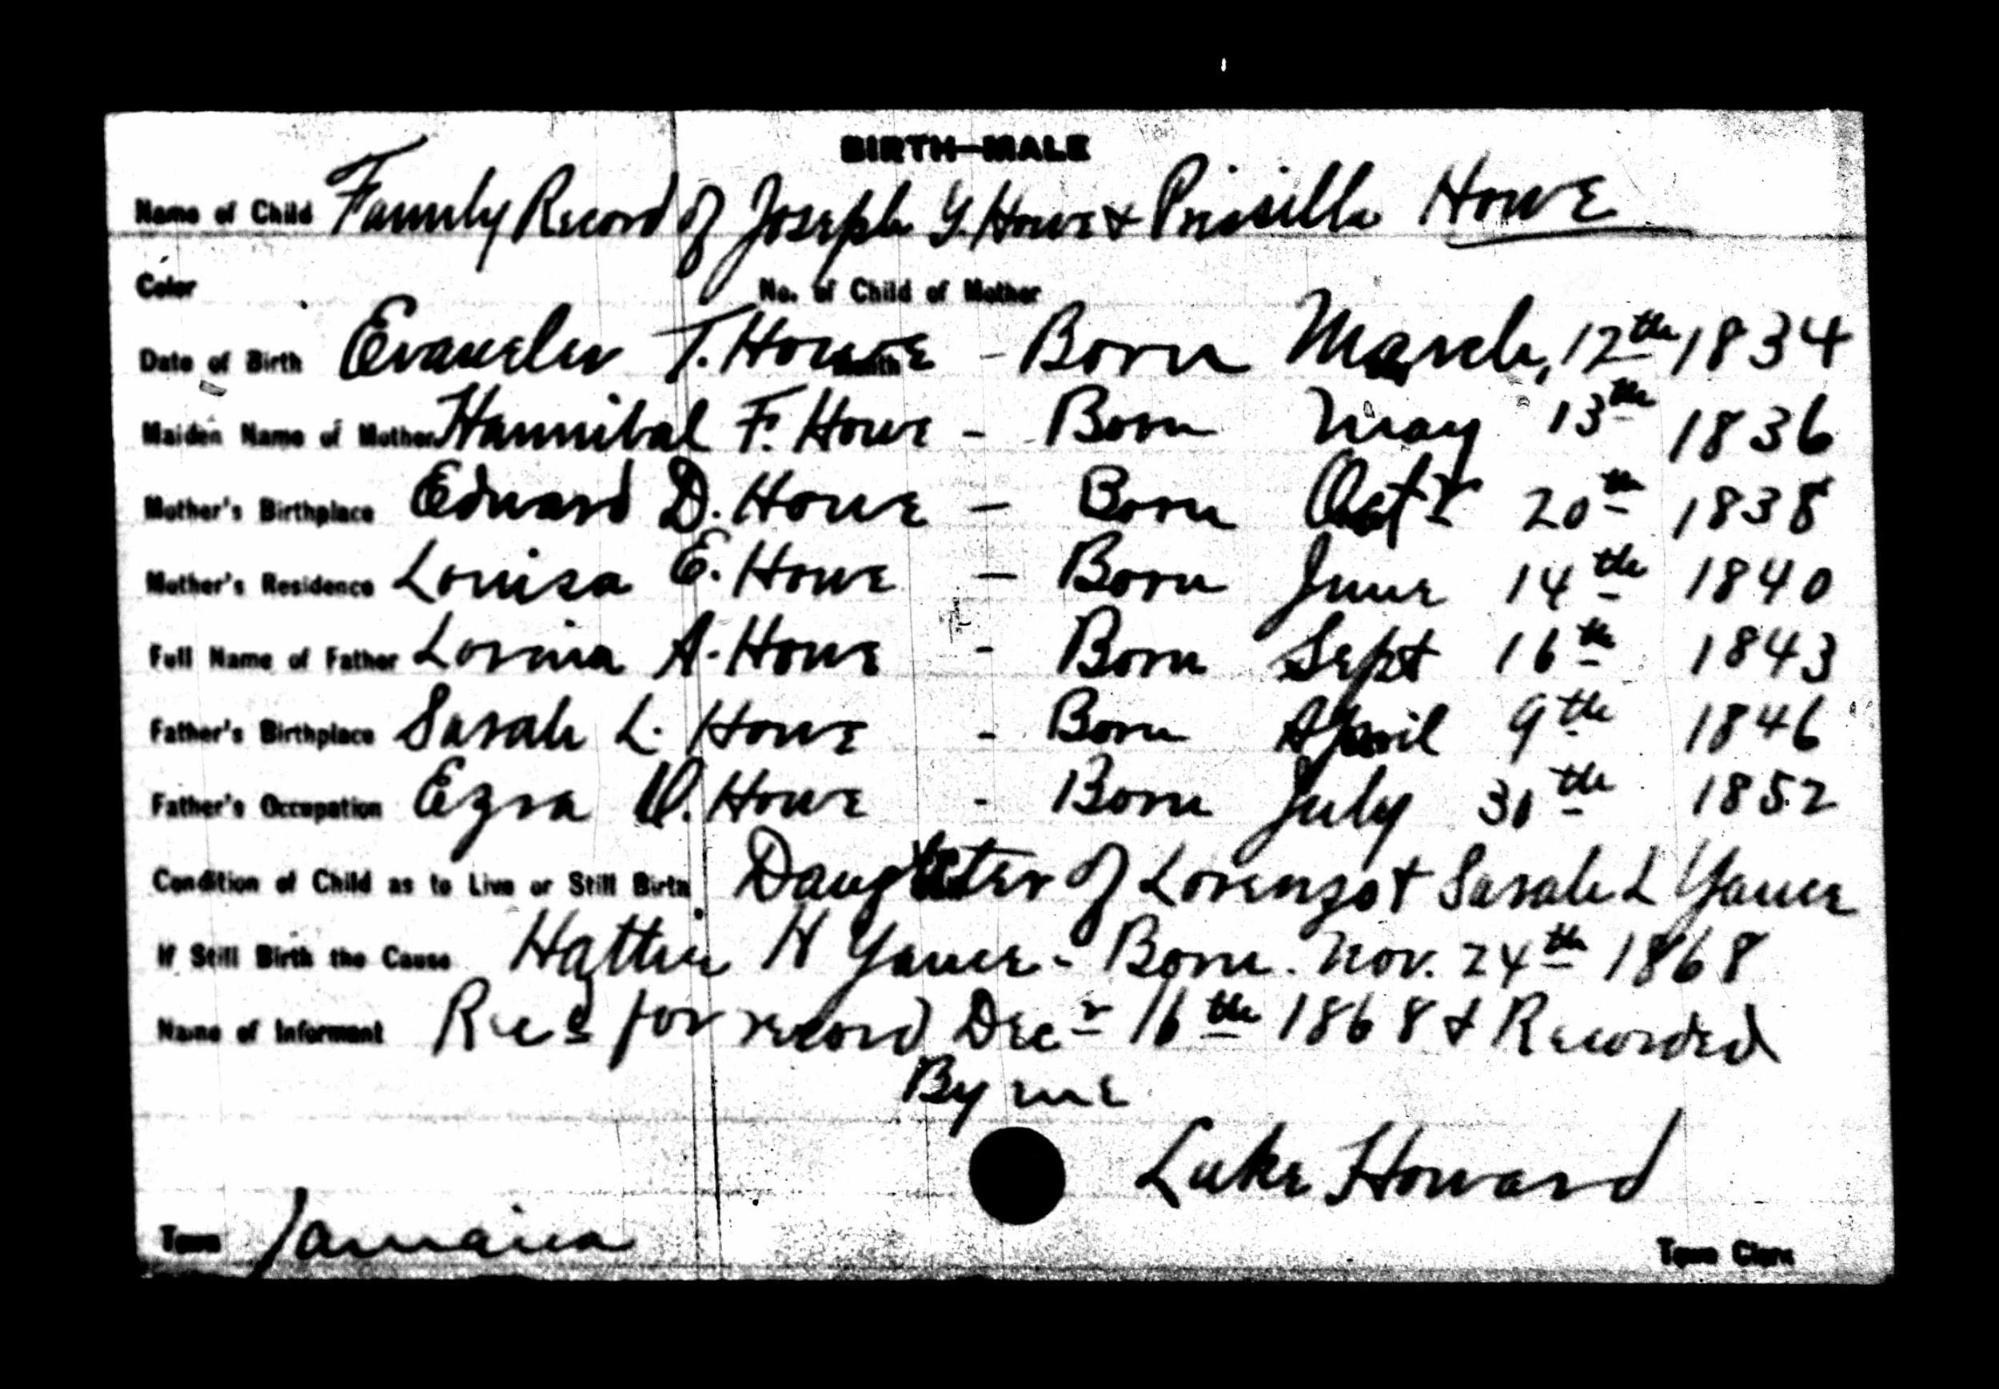
\includegraphics{images/0201b_images/image5.jpg}
\caption{alt\_text}
\end{figure}

\href{https://drive.google.com/file/d/0B94Urj3OjM7BekM0bEtsUWxjXzg/view}{https://drive.google.com/file/d/0B94Urj3OjM7BekM0bEtsUWxjXzg/vie}w

\hypertarget{references-3}{%
\subsection{References}\label{references-3}}

Eugene E. Snyder: \_We Claimed This Land: Portland's Pioneer Settlers, \_Binfort \& Mort Publishing, Portland, Oregon, 1989

Land Office, Saint Peter, Minnesota,\_ Military Warrant of 12/3/1860 for 120 acres in favor of Sarah Knecht.\_

\emph{\url{https://drive.google.com/open?id=1QZ0y2OJXy5cxz8sOOjw0Va6KYY8rtnbW}}

Land Office, Saint Peter, Minnesota, \emph{State Volume Patent of 10/1/1860 for 27.62 acres in favor of Evander Howe}.

\url{https://drive.google.com/open?id=1QetYocfLN9_erFqzhu5xIl1h1dIJkq8f}

Multnomah County Court, \emph{Probate Case 858, Estate of Evander Howe.}

\url{https://drive.google.com/open?id=1xs6X_Qrkn7oQ42qUxIBs0PgluGlfWPlM}

Eugene E. Snyder: \_We Claimed This Land: Portland's Pioneer Settlers, \_Binfort \& Mort Publishing, Portland, Oregon, 1989

General Land Office Records,\_ Copy of MN1220-00241, issued 10/01/1860.\_

\href{https://drive.google.com/file/d/1QetYocfLN9_erFqzhu5xIl1h1dIJkq8f/view}{https://drive.google.com/file/d/1QetYocfLN9\_erFqzhu5xIl1h1dIJkq8f}

General Land Office Records,\_ Copy of MW-0465-308, issued 12/03/1860.\_

\href{https://drive.google.com/file/d/1QZ0y2OJXy5cxz8sOOjw0Va6KYY8rtnbW/view}{https://drive.google.com/file/d/1QZ0y2OJXy5cxz8sOOjw0Va6KYY8rtnbW}

General Land Office Records,\_ Copy of OROCAA 040709, issued 06/01/1870.\_

\url{https://drive.google.com/file/d/0B94Urj3OjM7Bd0RkakpYTktEc2s}

Multnomah County Records,\_ Book I, Page 215, recorded 07/05/1870\_

\href{https://drive.google.com/file/d/1PiJlcxtVmqaULLe7XHCWsoMWEnVwgHo5/view}{https://drive.google.com/file/d/1PiJlcxtVmqaULLe7XHCWsoMWEnVwgHo5}

Multnomah County Records,\_ Book I, Page 247, recorded 07/12/1870\_

\url{https://drive.google.com/file/d/1PyOtjEaGyvoSKLLvfJP47aOp6nn6BtqY/view}

Multnomah County Records,\_ Book M, Page 56, recorded 11/05/1870\_

\url{https://drive.google.com/file/d/1Q1bc6cNj1x-ssB3AXnrFnUO2-VMFzShy/view}

Ancestry.com, \emph{Vermont Vital Records, 1720-1908}

\url{https://drive.google.com/file/d/0B94Urj3OjM7BeldUckFKSUx0blk/view}

Multnomah County Court, \emph{Probate Case 858, Estate of Evander Howe.}

\url{https://drive.google.com/open?id=1xs6X_Qrkn7oQ42qUxIBs0PgluGlfWPlM}

\hypertarget{homesteads-david-and-martha-jane-ulery}{%
\section{Homesteads: David and Martha Jane Ulery}\label{homesteads-david-and-martha-jane-ulery}}

\begin{figure}
\centering
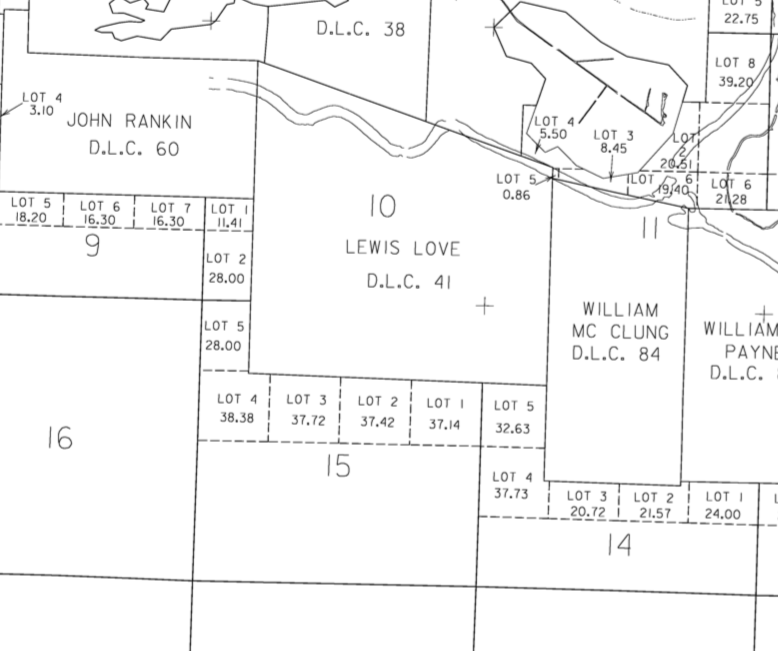
\includegraphics{images/0202a_images/image1.png}
\caption{alt\_text}
\end{figure}

\hypertarget{homestead-1}{%
\subsection{Homestead}\label{homestead-1}}

Between Bryant Street and Portland Boulevard (now Rosa Parks Way), from Union Avenue (now MLK) to what is now Missouri, were three lots of public land, each about 37 acres. Together with another 32 acre lot, numbered 5, in Section 14 (now in Woodlawn), they were included in a Military Bounty Land Warrant of 160 acres given to A-Chars-War-Chee (MW-0229-025, dd 12/10/1864), who immediately transferred the land to David Ulery (or Ullery).

\begin{quote}
\emph{To all to whom these Presents shall come, Greeting. Whereas, in pursuance of the Act of Congress, approved March 3, 1855, entitled ``An Act in addition to certain Acts granting Bounty Land to certain Officers and Soldiers who have been engaged in the military service of the United States'' there has been deposited in the General Land Office, Warrant No.~93230 for 160 acres, in favor of A Chars War Chee, Warrior Captain Paddy Carrs Company Creek Volunteers Creek War with evidence that the same has been duly located upon the fractional South East quarter of the North West quarter, the fractional South half of the North East quarter (or lots numbered one, two, and three) of Section Fifteen and the South West quarter of the North West quarter (or lot numbered five) in Section Fourteen in Township One North of Range One East in the district of lands subject to the sale at Oregon City Oregon containing one hundred and forty four acres and ninety one hundredths of an acre according to the Official Plat of the Survey of said Lands returned to the General Land Office by the Surveyor General. The said Warrant having been assigned by the said A. Chars War Chee to David Ulery in whose favor said tract has been located. }
\end{quote}

\begin{quote}
\emph{Now know ye that there is therefore granted by the United States unto the said David Ulery as assignee as aforesaid and to his heirs to tract of Land above described: To Have and To Hold the said tract of Land with the appurtenances thereof, until the said David Ulery as assignee as aforesaid and to his heirs and assign forever.}
\end{quote}

\begin{quote}
\emph{In testimony whereof, I, Abraham Lincoln, President of the United States of America, have caused these letters to be made patent, and the Seal of the General Land Office to be hereunto affixed.}
\end{quote}

\begin{quote}
\emph{Given under my hand, at the City of Washington, the tenth day of December in the year of our Lord one thousand eight hundred sixty four and of the Independence of the United States the Eighty Ninth. By the President (signed) Abraham Lincoln. By (signed) Edw D Neill, Sec'y. (signed) J.M. Granger, Recorder or the General Land Office.}
\end{quote}

\begin{verbatim}
_[https://drive.google.com/open?id=0B94Urj3OjM7BczdjVDk0NlZJMmc](https://drive.google.com/open?id=0B94Urj3OjM7BczdjVDk0NlZJMmc)_
\end{verbatim}

The tax lots are more clearly shown on the map below. Note that tax lots 4 and 5 on the west side of section 15, which includes the small strip of modern Piedmont between Missouri and the freeway, were in the homestead of John Fenstermacher.

\begin{figure}
\centering
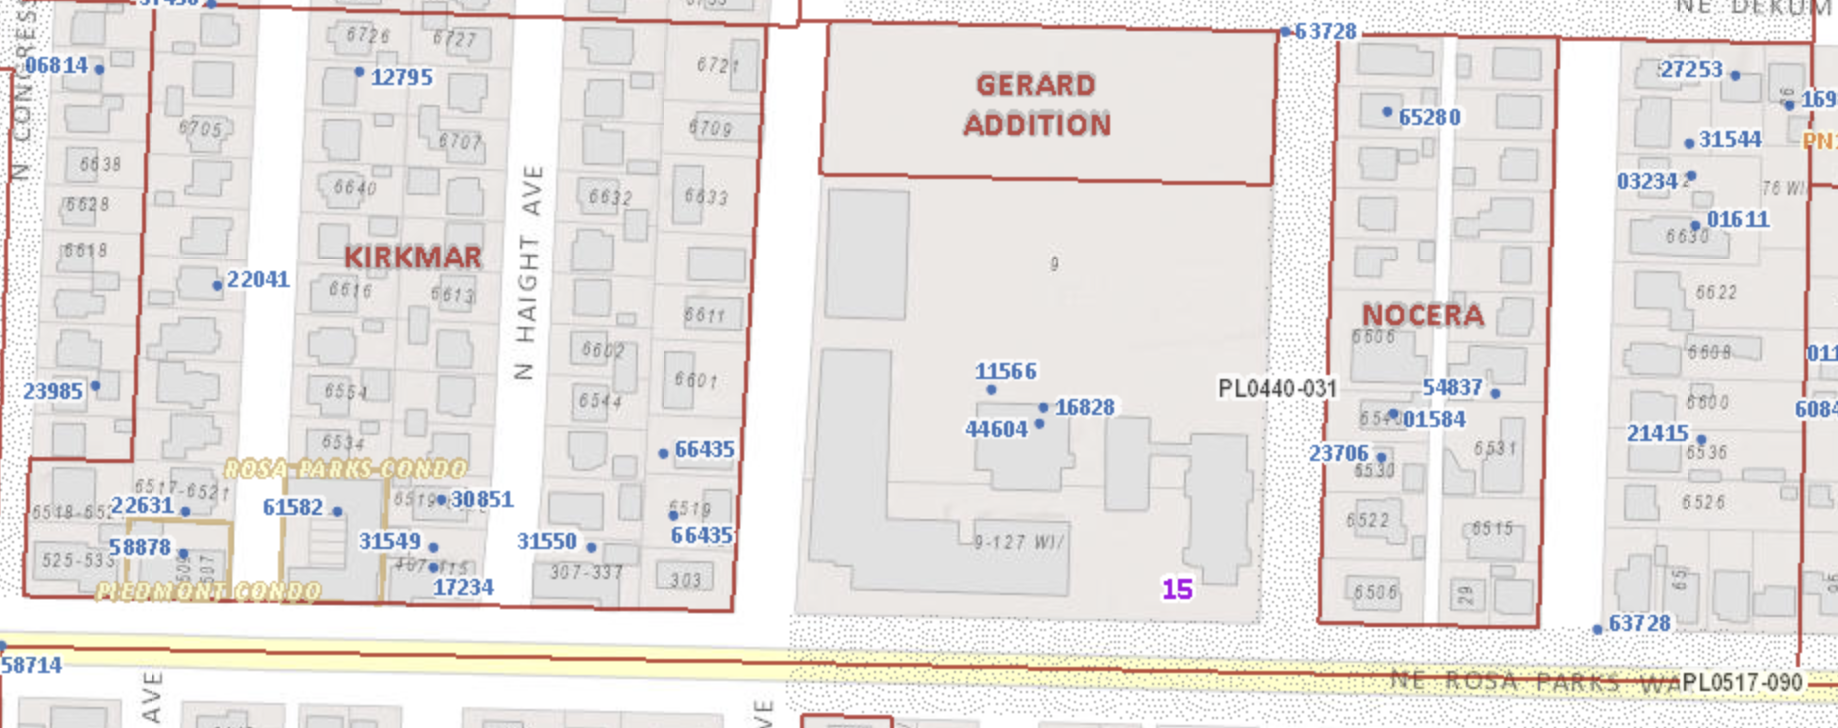
\includegraphics{images/0202a_images/image2.png}
\caption{alt\_text}
\end{figure}

In 1882 Ulery sold his Portland properties and moved to the Chelatchie Valley in Clark County. On the David Ulery DLC the subdivisions of Beverly, Piedmont Park, Parkway, Saratoga, Nocera, Kirkmar, Gem Addition, Rose Addition, Lochinvar, Lahoma, and Cumberland were created.

\hypertarget{sales-first-phase}{%
\subsection{Sales (First Phase)}\label{sales-first-phase}}

On May 2, 1863 David and Martha Jane Ulery sold part of their land to John Hotts. Note that this was even before the land was formally assigned to David Ulery by the United States. Here is the deed.

\begin{quote}
\emph{This indenture witnesses that we David Ulery and Martha Jane Ulery his wife for the consideration of Sixty two dollars to us paid have bargained and sold and by those presents do bargain, sell and convey to John Hotts the following described premises to wit: the fractional South East quarter of the North West quarter in Section fifteen in Township One North of Range One East containing thirty seven acres and seventy two one hundredth. To have and to hold the said premises with their appurtenances unto the said John Hotts his heirs and assigns forever. And I the said David Ulery do hereby covenant to and with the said John Hotts his heirs and assigns that I am the owner in fee simple of said premises, that they are free of all encumbrances and that I will warrant and defend the same from all lawful claims whatsoever. Witness our hands and seals this 2nd day of May AD 1863. (signed) David Ulery (signed) Martha Jane Ulery}
\end{quote}

\begin{verbatim}
_[https://drive.google.com/file/d/1Q2f1OAYB4G4sSQ5DH9SI9wLx5rS2DrEa](https://drive.google.com/file/d/1Q2f1OAYB4G4sSQ5DH9SI9wLx5rS2DrEa)_
\end{verbatim}

It is pretty clear from this description that what was sold here is what is lot 3 on the map, the most western part of the DLC.

In the second step the Ulery's sold lot 5, the part in Section 14, currently in Woodlawn, to Silas Jones for \$ 1,050. The deed was recorded on December 19, 1881.

\url{https://drive.google.com/open?id=1C2Y59TD9k1_Jpt4FgoAvi7_1Oyme24PM}

The next deed records the sale of 25 acres to Lewis Washington Love, son of William Love, and grandson of Lewis Love. It was recorded on February 1, 1882.

\begin{quote}
\emph{Know all men by these Presents : That we David Ulery and Martha J Ulery wife of said David Ulery of the County of Multnomah and State of Oregon, in consideration of Seven hundred (700) dollars to us paid by Lewis W. Love of said Multnomah County State of Oregon do hereby grant bargain sell and convey to said Lewis W. Love and to his heirs and assigns forever the following described parcel of real estate to wit: Being a part of Section Fifteen (15) in Township One (1) North Range One (1) East of Willamette Meridian and bounded as follows to wit: Beginning at a stake on the boundary line between sections fourteen (14) and fifteen (15) in said Township and on the South boundary of the Lewis Love Donation Land Claim and running from thence South eighteen (18) chains and eighteen (18) links to the quarter Section post between said sections fourteen and fifteen. Thence West thirteen chains (13) and seventy five (75) links to a post. Thence North eighteen (18) chains and thirteen (13) links to the South boundary of said Love land claim. Thence East along the South boundary of said land claim thirteen (13) chains and Seventy five links to the place of beginning, containing twenty five acres of land in the said County of Multnomah State of Oregon.}
\end{quote}

\begin{verbatim}
[https://drive.google.com/open?id=1Pkg_9J7pJbt2aGqM71KIZp8SUPG3_Gp9](https://drive.google.com/open?id=1Pkg_9J7pJbt2aGqM71KIZp8SUPG3_Gp9)
\end{verbatim}

To translate 18 chains and 18 links is 1200 feet, 18 chains and 13 links is 1196.6 feet, and

13 chains and 75 links is 907.5 feet. Thus basically this is the east 25 acres of lot 1. The next three deeds were also recorded on February 1, 1882. We transcribe the key parts.

\begin{quote}
\emph{Know all men by these Presents : That we David Ulery and Martha J Ulery wife of David Ulery of the County of Multnomah and State of Oregon, in consideration of Twelve hundred \textless1200\textgreater{} dollars to us paid by Florence Meade of the said Multnomah County State of Oregon do hereby grant bargain sell and convey to said Florence Mead and to her heirs and assigns forever the following described parcel of real estate to wit: Being a part of Section Fifteen \textless15\textgreater{} in Township One \textless1\textgreater{} North Range One \textless1\textgreater{} East of Willamette Meridian and bounded as follows to wit: Beginning at a post in the Center of the Vancouver road said post being in the South boundary line of the Lewis Love Donation Land claim eighteen \textless18\textgreater{} chains and sixty seven \textless67\textgreater{} links North of the Stone monument at the center of Section Fifteen \textless15\textgreater{} in Township one North Range One \textless1\textgreater{} East Willamette Meridian and Eleven \textless11\textgreater{} chains and Seventy five \textless75\textgreater{} links Easterly of said monument and running from thence South forty five \textless45\textgreater{} minutes West along the Vancouver County Road nine \textless9\textgreater{} chains and eighteen (18) links to the North line of a certain twenty five (25) acre tract. Thence East along the North line of said tract fifteen chains to a point thence North Eight \textless8\textgreater{} chains and Eighty \textless80\textgreater{} links to the South line of the Lewis Love Donation Land Claim thence North 89 degrees 30 minutes West along the said boundary line of said Love claim fourteen \textless14\textgreater{} chains and 99 links to the place of beginning containing 13 38/100 acres of land.}
\end{quote}

\begin{verbatim}
_[https://drive.google.com/open?id=1Q3cmINUpsdgSevedjngBoH8ntSKsPnmE](https://drive.google.com/open?id=1Q3cmINUpsdgSevedjngBoH8ntSKsPnmE)_
\end{verbatim}

\begin{quote}
\emph{Know all men by these Presents : That we David Ulery and Martha J Ulery wife of the said David Ulery of the County of Multnomah and State of Oregon, in consideration of Twenty five hundred \textless2500\textgreater{} dollars to us paid by Sarah McMillen of the said Multnomah County State of Oregon do hereby grant bargain sell and convey to said Sarah McMillen and to her heirs and assigns forever the following described parcel of real estate to wit: situated in the said County of Multnomah and bounded as follows: Beginning at a Stone in the center of Section Fifteen \textless15\textgreater{} in Township One North Range One \textless1\textgreater{} East: thence East twenty six chains and 62 links to a post; thence North nine (9) chains and thirty nine \textless39\textgreater{} links to a post; thence West parallel with the South side line twenty six chains and sixty two (62) links to a stone; thence South Nine \textless9\textgreater{} and thirty nine \textless39\textgreater{} links to the place of beginning containing twenty five acres of land.}
\end{quote}

\begin{verbatim}
_[https://drive.google.com/open?id=1Q2rR3Q3QsmvySkHXgdclIzCoOZTP -QNl](https://drive.google.com/open?id=1Q2rR3Q3QsmvySkHXgdclIzCoOZTP-QNl)_
\end{verbatim}

\begin{quote}
\emph{Know all men by these Presents : That we David Ulery and Martha J Ulery of the County of Multnomah and State of Oregon (Martha J. Ulery being the wife of the said David Ulery), in consideration of Twelve hundred \textless1200\textgreater{} dollars to us paid by Terzah B. McMillen of the said County of Multnomah do hereby grant bargain sell and convey to said Terzah B. McMillen and to her heirs and assigns forever the following described parcel of real estate to wit: situated in the said County of Multnomah State of Oregon and bounded by beginning at a point nine (9) chains and thirty nine (39) links North of a stone set at the center of Section fifteen in Township one (1) North Range one (1) East and running from thence north nine (9) chains and twenty eight (28) links to the stone monument in the South boundary line of the Lewis Love Donation Land Claim. Thence South 89 degrees (89˚) and thirty (30) minutes (30') East along said Donation Claim line eleven chains and seventy five (75) links to center of Vancouver County Road. Thence South 45 minutes (0˚ 45') W. nine (9) chains and eighteen (18) links to the north line a certain twenty five acre tract, thence west eleven (11) chains and sixty two (62) links to the place of beginning containing ten acres and seventy seven hundredths of land.}
\end{quote}

\begin{verbatim}
_[https://drive.google.com/open?id=1Q10BF7FtoueSKOO9elULOmFD2L23xo1S](https://drive.google.com/open?id=1Q10BF7FtoueSKOO9elULOmFD2L23xo1S)_
\end{verbatim}

I can summarize all four transactions in a picture, showing how tax lots one, two, and three were divided. I used a modern map to draw the boundaries on, but of course none of the streets were there in 1882, except Vancouver Road. Also, there is no guarantee that the boundaries are precise to within the millimeter, but it's a pretty good approximation.

\begin{figure}
\centering
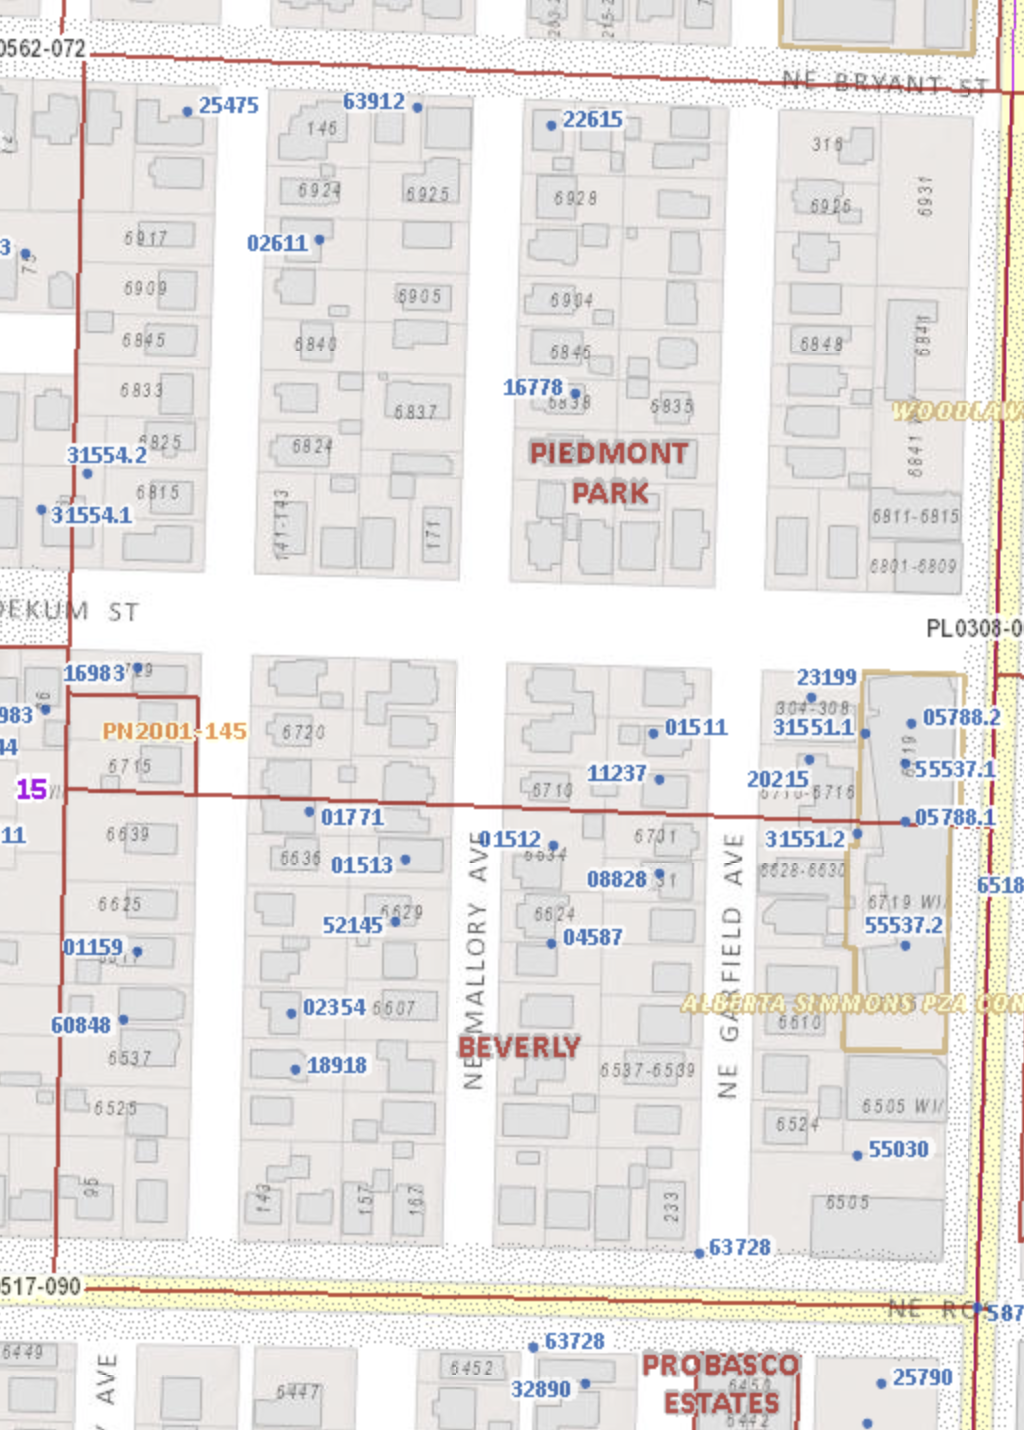
\includegraphics{images/0202a_images/image3.png}
\caption{alt\_text}
\end{figure}

\begin{verbatim}
[https://drive.google.com/open?id=18J7V0CGXE1adVcPZOBAwwANgSH4XmGJj](https://drive.google.com/open?id=18J7V0CGXE1adVcPZOBAwwANgSH4XmGJj)
\end{verbatim}

Compare this with a modern subdivision map. We see that the Lewis Love piece was subdivided into Beverly and Piedmont Park. The Florence Mead part became Saratoga. The Sarah McMillen part became Kirkmar, Nocera, and the Gerard Addition, as well as the Holy Redeemer complex. The Terzah McMillen part became the Gem Addition and Devine's Addition. The John Hotts part became Lahoma, Lochinvar, Cumberland, Pacific Place, Parkway, New Albina, and the Rose Addition.

\begin{figure}
\centering
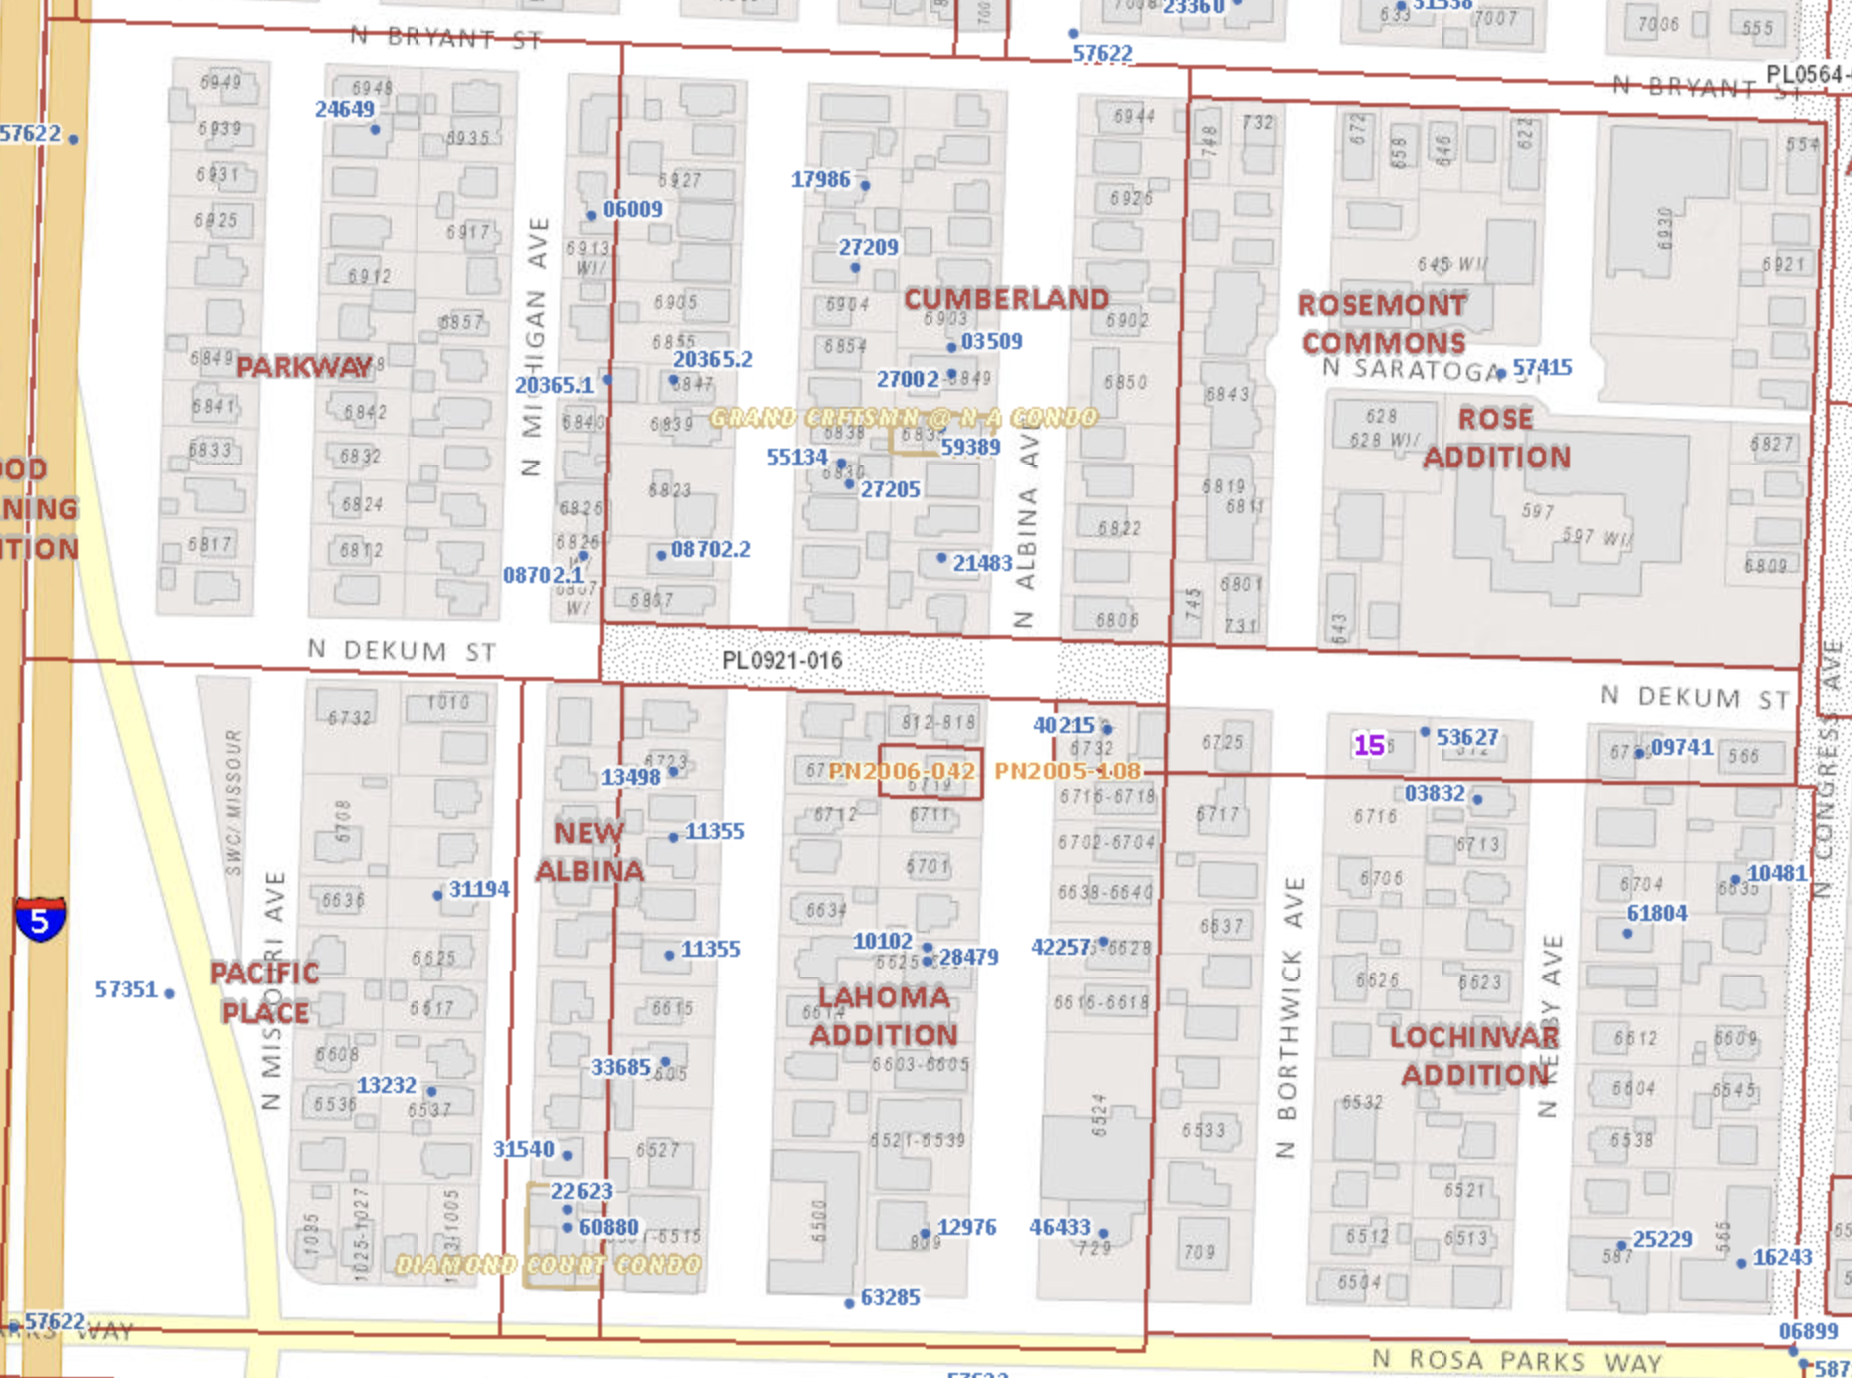
\includegraphics{images/0202a_images/image4.png}
\caption{alt\_text}
\end{figure}

The David Ulery homestead illustrates clearly the general mechanism of larger pieces of land being sold in smaller pieces, introducing more owners, and eventually resulting in many subdivisions from a small number of homesteads. More to the north the Lewis Love DLC was partitioned into relatively large pieces, but the David Ulery DLC became fractured early on. This partitioning into subdivisions also allows us to answer discomforting existential questions such as ``Why does NE Rodney Ave not continue in a straight line at Bryant ?'' or ``Why does NE Saratoga St stop at its east end before it gets to NE Rodney Ave ?''.

\hypertarget{sales-second-phase}{%
\subsection{Sales (Second Phase)}\label{sales-second-phase}}

In the first phase of sales we started with a military donation claim of 144 acres, consisting of four tax lots of 37 acres. It was divided into six parcels, of which five were in the modern Piedmont neighborhood. As I indicated in the introduction, I will actually try to follow the title chains to the next level, where these five larger parcels will be partitioned into subdivisions. Bear with me, this will get complicated.

Nobody in the first set of buyers (John Hotts, Sarah McMillen, Terzah McMillen, Florence Meade, Lewis Washington Love) thought of actually platting and developing the land. The second phase started at the time of the consolidation of Albina, the relentless boosting by McKenna, Killingsworth, and Quackenbush, and the coming of bridges, railways, and streetcars on the East Side. All these parcels rapidly went up in value when Piedmont was platted in 1889. Sales picked up, plats were filed, and early investors made a nice profit. In many cases buyers sold in the same year they bought, and nevertheless making a considerable profit.

\hypertarget{lewis-washington-love}{%
\subsubsection{Lewis Washington Love}\label{lewis-washington-love}}

\begin{figure}
\centering
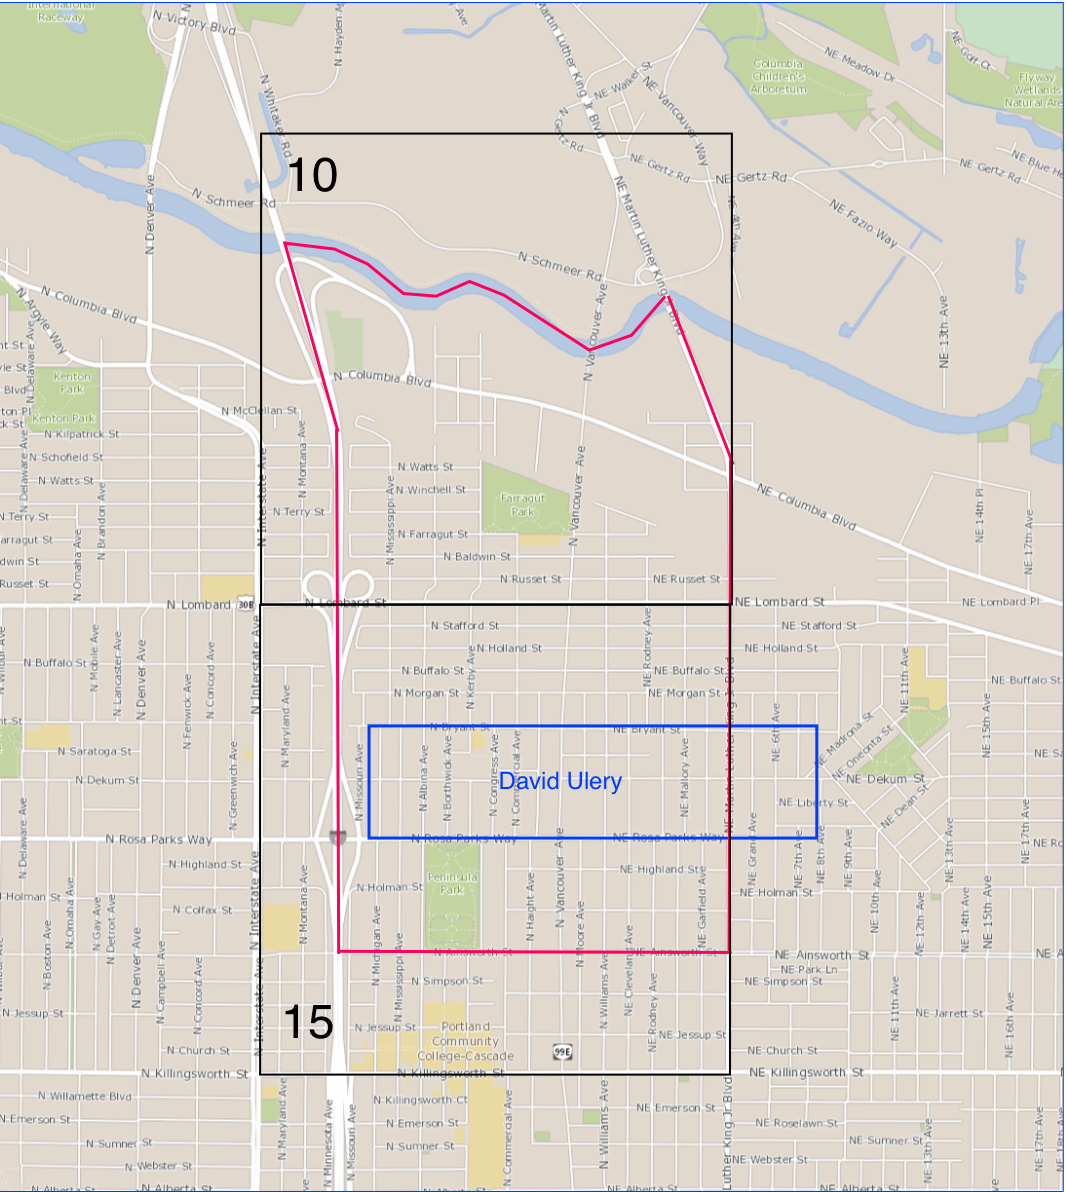
\includegraphics{images/0202a_images/image5.png}
\caption{alt\_text}
\end{figure}

Let's start with the twenty five acres that Lewis Washington Love bought from Ulery. He sold them for \$ 3,125 to W. G. Jenne on September 22, 1882.

\url{https://drive.google.com/open?id=1AeyvCQDgk2Hzsy2hiAAmePk9hGdAOprF}

\hypertarget{piedmont-park}{%
\paragraph{Piedmont Park}\label{piedmont-park}}

On February 20, 1889 W. G. and Ida J. Jenne sold the northern 15 acres, the section that would become Piedmont Park, to G. W. Stearns for \$ 7,500.

\url{https://drive.google.com/open?id=1Bnm-HAauK5hZohLcjlSqln5wZOVRW13f}

There is an interesting clause in the deed.

\begin{quote}
\emph{\ldots{} together with the right of road over the east 30 feet of the 10 acre tract of land adjoining the south boundary of above conveyed tract of land and saving and excepting a like right of road over the said 15 acre tract above conveyed, said rights to last till both of said tracts are made accessible by public road to both the Woodlawn Station and the Vancouver road and no longer.}
\end{quote}

G. W. and Josephine C. Stearns in turn sold the parcel for \$ 9,000 to D. B. Monteith on February 26, 1889.

\begin{verbatim}
[https://drive.google.com/open?id=1ML8wCkaoPr79fW_hHkGa82QVcbPMWRlj](https://drive.google.com/open?id=1ML8wCkaoPr79fW_hHkGa82QVcbPMWRlj)
\end{verbatim}

And D. B. and Irma M. Monteith sold to J. P. and Louise M. Menefee, F. W. and Ida E. Torgler, and Charles C. and Emma Woodcock on February 23, 1891 for \$ 13,500.

\url{https://drive.google.com/open?id=12pittgegX7YngO43wen-8rmJCq2ReQFd}

Those same three couples filed the plat for Piedmont Park on June 5, 1891.

\hypertarget{beverly}{%
\paragraph{Beverly}\label{beverly}}

The southern 10 acres were more of a problem. I have not figured this one out completely yet. Clearly Jenne was unable or forgot to pay his property taxes, because Sheriff George C. Sears sold the parcel on November 26, 1894 to E.S. Rash for \$ 50.00.

\url{https://drive.google.com/open?id=1c_R6kSraX5bRp-F_YsVsRYNX86PdHE6-}

\url{https://drive.google.com/open?id=18GqNBpgRIBQskNp7KwteuuQvzoJh2xT1}

\hypertarget{florence-meade}{%
\subsubsection{Florence Meade}\label{florence-meade}}

\begin{figure}
\centering
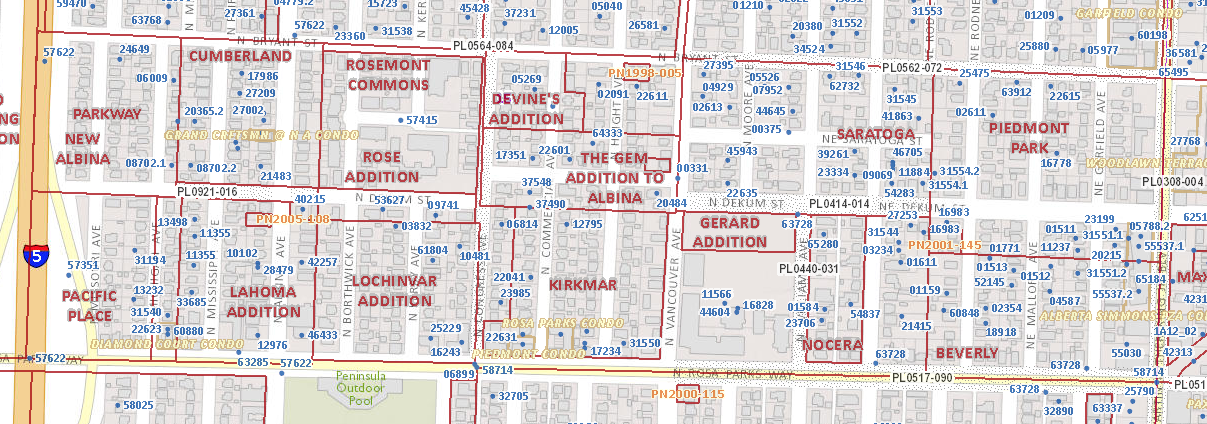
\includegraphics{images/0202a_images/image6.png}
\caption{alt\_text}
\end{figure}

\hypertarget{saratoga}{%
\paragraph{Saratoga}\label{saratoga}}

The 13.38 acres that are now Saratoga have a relatively simple story. We have seen they were sold by the Ulery's to Florence Meade for \$ 1,200 on February 1, 1882. W. H. and Florence Meade in turn sold them for \$ 2,750 to Julius E. Sorbin of Albany on October 17, 1882.

\url{https://drive.google.com/open?id=1KLX7BJODfJs3j9rXvTBeuPeE3nSyj8CU}

Sorbin quitclaimed them to Hardy C. Wortman for \$ 1.00 on March 28, 1889.

\url{https://drive.google.com/open?id=15YaEpNWuV32RXssr8tE_Rjedt8inY-bL}

And finally Wortman filed the plat for Saratoga on March 30, 1889. Both Mr.~Wortman and the Saratoga subdivision have their separate chapters in this book.

\hypertarget{sarah-mcmillen}{%
\subsubsection{Sarah McMillen}\label{sarah-mcmillen}}

\begin{figure}
\centering
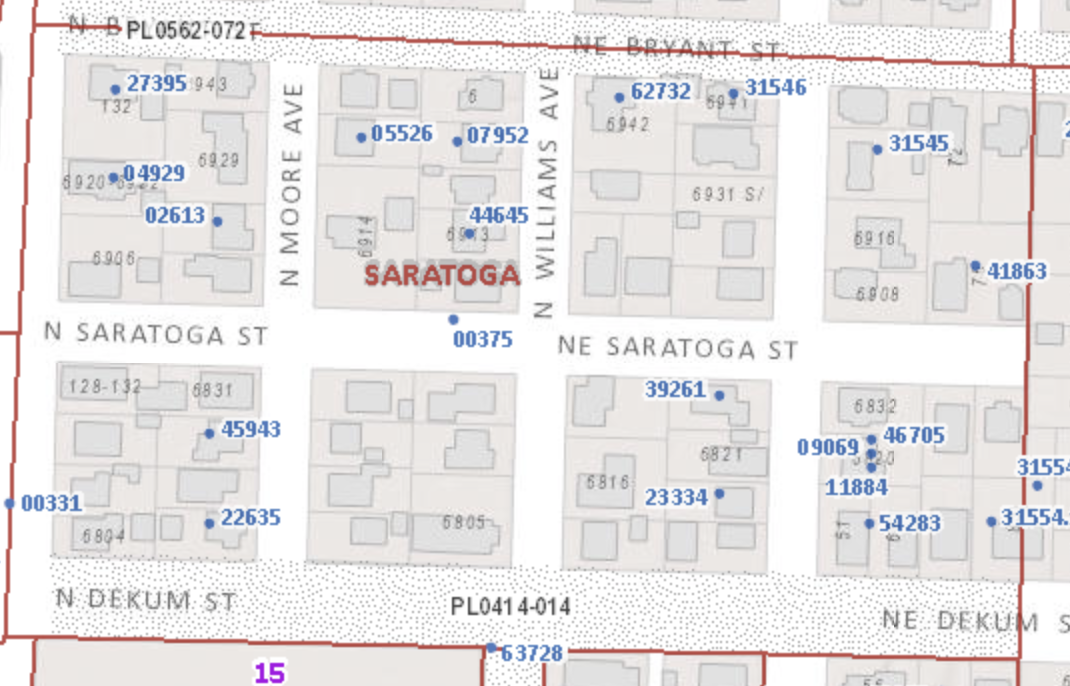
\includegraphics{images/0202a_images/image7.png}
\caption{alt\_text}
\end{figure}

The 25 acres that Sarah McMillen bought from the Ulery's for \$ 2,500 on February 1, 1882 were transferred on August 5 of the same year by R. H. McMillen and his wife Sarah to Orlando Rossi for \$ 3,750.

\url{https://drive.google.com/open?id=1eGovVTgQl9t6wy-RwZT-0hLwj5jQFX-Q}

On August 29 of 1882 Orlando and Mathilda Rossi sold the parcel for \$ 5,000 to George Marshall.

\url{https://drive.google.com/open?id=1yxfTlUA1IIOKgnwmR2iNfxqZSC1MQR1w}

The next transaction I have found is a quitclaim for \$ 1.00 by George Marshall to his wife Margaretta Kirk-Marshall on April 30, 1884.

\url{https://drive.google.com/open?id=1TJT-hBNQ5H1WqyNsFAb-PZg9TLSq3NFi}

The Marshall family, who have their own chapter in this book, were in the habit of transferring their real property to other members of the family when they got older and/or sicker, probably to avoid probate, executors, appraisers, and taxes. The probate file for George Marshal shows basically that at his death there was nothing left in the estate, and the executor of the estate (his wife) had an easy job.

\url{https://drive.google.com/open?id=1sHPTMHOAw8sQwdT8zWILltRa6XS1AZS7}

\hypertarget{kirkmar}{%
\paragraph{Kirkmar}\label{kirkmar}}

There are two Margaretta Marshalls to be considered. The first is Margaretta Kirk-Marshall, who died in 1897. She left an estate worth almost \$ 100,000, mostly consisting of real property, but the parcel in the Piedmont Neighborhood was not mentioned in the probate file.

\url{https://drive.google.com/open?id=1f7eJnJneqAYa3_yv-8K96VM1CYHH2O96}

The second Margaretta is the daughter Margaretta A. Marshall, who in April 1929, with her sister Vidae L. Marshall and her niece M. Genevieve Jones, platted the 8.08 acres of the western part of the Sarah McMillan parcel, between Congress and Vancouver, as Kirkmar. Presumably the name Kirkmar is derived from Kirk-Marshall.

The 100 by 450 feet chunk (1.03 acres) at Congress ? Why ? Must have been sold by Marshall's rather early on.

\hypertarget{nocera}{%
\paragraph{Nocera}\label{nocera}}

The eastern part. First the 2 ⅚ acres that later becomes Nocera.

\begin{quote}
\emph{Beginning on the quarter section line running east and west through the center of section 15, in Township one (1) north of range one (1) east, at a point 1130 feet west of the east line of said section; which said point is at the southwest corner of a parcel of land containing three and one-sixth (3 ⅙) acres heretofore conveyed to one Gustave M. Keller and running thence north six hundred nineteen and 74/100 (619.74) feet; thence west on a line parallel with said quarter section line two hundred (200) feet; thence south six hundred nineteen and 74/100 (619.74) feet; thence east and along said quarter line two hundred (200) feet to point of beginning, containing two and five-sixths (2-⅚) acres of land, be the same more or less.}
\end{quote}

Helen O. Stoppenbach for \$ 5,000 to the Reverend William T. Bond on May 17, 1906, Book 364 Page 48

\url{https://drive.google.com/open?id=15h9n3ps0Xf5Zyjhc5jJUFv3j13Zqq7DX}

The Reverend William T. Bond, unmarried, of Kansas City, Missouri to the Very Reverend Joseph A. Firle of St.~Louis, Missouri for \$ 5,000 on March 4, 1907.

\url{https://drive.google.com/open?id=1U9152Iczi_eLQgW73VpOKRD_xwpMGy9g}

The Provincial of the order, the Very Reverend Joseph A. Firle, unmarried, of St.~Louis, Missouri to Society of Redemptorists Fathers for \$ 10 on July 18, 1907.

\url{https://drive.google.com/open?id=1hURir6D96BavyHG9oqakCxs2gPfTxDSp}

Also: June 1806, Redemptorist Fathers William Bond and Joseph Bell bought 6 acres for \$ 12,000. Monday Oregonian March 15, 1907. (??)

On March 6, 1907 Mary E. Marsh, Margaretta Marshall, and Vidae L. Marshall (all unmarried) sold 8.2936 acres to the Redemptorist Fathers for \$ 18,622.28 dollars

\url{https://drive.google.com/open?id=1BMJ_4OM8acJgwgkpoWRBK10Msji5zy-S}

And then there is Gustave Keller. He bought the easternmost 3 ⅙ acres of the Sarah McMillen tract from Mary E. Marsh, Margaretta Marshall, and Vidae L. Marshall for \$ 1058,33 on April 9, 1908.

\url{https://drive.google.com/open?id=1TJrNLv0tHmmLgt_N9R_H-LDtXD-Dq5qB}

This part was never platted. There is some interesting history here, which we review in the chapter on Gustave and Amalia Keller.

\hypertarget{terzah-b.-mcmillen}{%
\subsubsection{Terzah B. McMillen}\label{terzah-b.-mcmillen}}

\begin{figure}
\centering
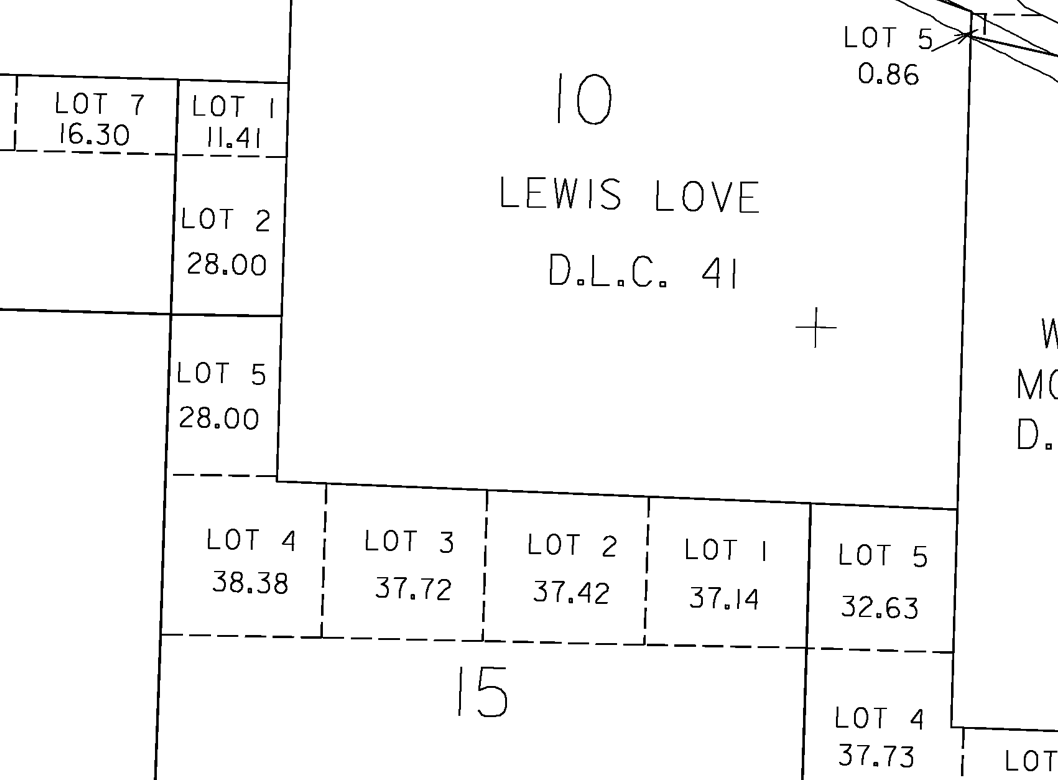
\includegraphics{images/0202a_images/image8.png}
\caption{alt\_text}
\end{figure}

South 5.385 acres of 10.77 acres. Becomes Gem Addition.

The undivided one half from James H. and Terzah B. McMillen to George F. Wells and V. K. Strode for \$ 1,500 on January 3, 1883.

\url{https://drive.google.com/open?id=1Gra4CIM3rgHxwfN4J5JuyxxlbXxuikwn}

The south half from V. K. and Katie Strode and George F. and Lizzie Wells to Mark Jarrett for \$ 1,614.00 on October 16, 1888.

\url{https://drive.google.com/open?id=1VgbMb9qrlMiRiMfEJcU_UXwGCVlHaAYZ}

Trust deed for the southern 5 acres Lula J. Jarrett to Henry George, Bk 121 Page 437. April 15, 1889.

Henry A. and M. V. George quitclaim for \$ 10 to Lula J. Jarrett on October 30, 1889.

\url{https://drive.google.com/open?id=1TxO8fdHAkJtmOyeUNV9-jV2b19j7IsBk}

Lula J. Jarrett to William Kincaid 5.38 acres for \$ 1 on February 25, 1890.

\href{https://drive.google.com/file/d/1Kk6QgcMRFPnn1U6JgP681X-UaxYRIxYK/view?usp=sharing}{https://drive.google.com/file/d/1Kk6QgcMRFPnn1U6JgP681X-UaxYRIxYK}

Charles K. and Lydia Henry plat the Gem Addition to Albina on March 24, 1890.

Northern half: becomes Devine's Addition (about 2.2 acres).

Mary C. and George E. Smith 3 acres to Rose A. Woodard on May 12, 1903 for \$ 3,150.

\url{https://drive.google.com/open?id=1CWTgQaaESLtU0QzNMSPYMlBYnudLkRtg}

Mary C. and George E. Smith 2.2 acres to Patrick J. Devine on April 1, 1909 for \$ 10.

\href{https://drive.google.com/file/d/1_WYa6Eh2yAGG_scNXSjRWUi_vrLYDm0y/view?usp=sharing}{https://drive.google.com/file/d/1\_WYa6Eh2yAGG\_scNXSjRWUi\_vrLYDm0y}

Patrick J. and Minnie E. Devine platted on June 17, 1909.

\hypertarget{john-hotts}{%
\subsubsection{John Hotts}\label{john-hotts}}

\begin{figure}
\centering
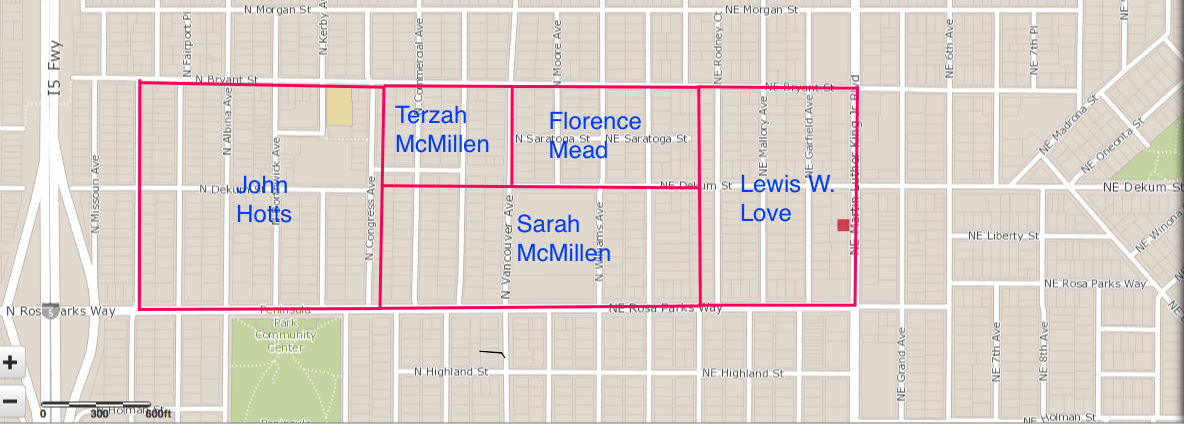
\includegraphics{images/0202a_images/image9.png}
\caption{alt\_text}
\end{figure}

If you think the second wave of sales was complicated for the McMillen pieces, then wait till you hear what happened to the 37.72 acres sold (for \$ 62) to John Hotts. I am still pretty far from resolving all the transactions for that parcel between 1882 and the final plats around 1920, but eventually I'll get there.

It started out relatively simple. On December 27, 1882 John Hotts sold 40 acres to a consortium consisting of L. D. Brown, J. A. Strowbridge, H. J. Morrison, James C. Tolman, Edmond F. Lewis, and William P. Wright. The first four had an undivided ⅕ interest, Lewis and Wright had an undivided 1/10 interest.

\url{https://drive.google.com/open?id=1VHw9Ig8Qpyy7W0kbQzZjydlQs7z2-bJy}

Now, of course, 40 acres is more than 37.72 acres. No magick was involved, however. In 1862 John Hotts had also bought from John Finstermacher the 67.38 acres that bordered the Ulery homestead on the west side. Remember the DLC map I already showed earlier in this chapter. Tax lots 1, 2, 3, and 5 south of the Lewis Love DLC are Ulery's homestead, while lot 5 to the west of the Love DLC is in Finstermacher's homestead. Things become complicated because of lot 4 in the southwest corner, which is in Finstermacher's homestead, but is not entirely to the west of Love. The part that is south of the Love DLC is exactly the part in the current Piedmont neighborhood. On modern maps the south boundary of both Ulery and Finstermacher is Rosa Parks Way. The north boundary of Ulery is Bryant Street and the north boundary of Finstermacher's lot 5 is Lombard Street.

\begin{figure}
\centering
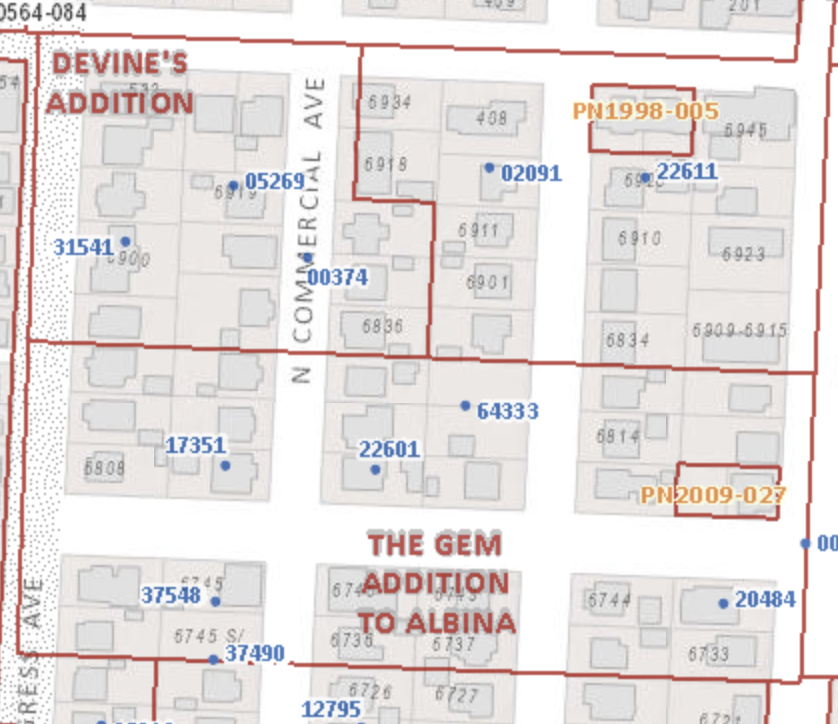
\includegraphics{images/0202a_images/image10.png}
\caption{alt\_text}
\end{figure}

Story of New Albina.

\hypertarget{rose-addition.}{%
\paragraph{Rose Addition.}\label{rose-addition.}}

May Harley from Sheriff (sale Watson, Watson Watson, Watson), October 6, 1896

Sold by Livingston Jenks and May Harley Jenks on December 5, 1905 to Arthur P. Prier for \$ 5,500.

\url{https://drive.google.com/open?id=1IUIYbru9DtI8wBql3fXXvqjkGdaPmjMy}

Then on March 27, 1907 sold by Arthur P. and Josie Prier to Margaret Dossche for \$ 12,000.

\url{https://drive.google.com/open?id=14heoBsdr6XJx65DFX_0k7fq8UJyLRWWB}

May 1907, Margaret Dossche to James Harvey Black, for \$ 10.

On November 22, 1907 sold by James Harvey Black (rector of St.~Francis) for \$ 100 to House of Good Shepherd, an Oregon company that platted the Rose Addition on May 10, 1917.

\url{https://drive.google.com/open?id=1TmQr9JkJx4O5-ma_pvrHRoa5nd5YsE7c}

8.02 acres that would become Lochinvar. Sold on October 23, 1889 for \$ 1 by J. M. Shelby (unmarried) and James M. and Lena Vanduyn to Francis I. McKenna. I am not sure about the wheeling and dealing that went on, but McKenna deeded

who platted Lochinvar on October 25, 1889.

3.72 acres Alice M. Allen. Tax deficiency. Sold to Ernest Cawston (her brother) Feb 1905.

\hypertarget{homesteaders-david-and-martha-jane-ulery}{%
\section{Homesteaders: David and Martha Jane Ulery}\label{homesteaders-david-and-martha-jane-ulery}}

\hypertarget{paddy-carr}{%
\subsection{Paddy Carr}\label{paddy-carr}}

We have seen that military bounty land was often passed on by the beneficiaries, undoubtedly for a small fee, to persons with more money and more of an idea of what to do with the land. This was certainly the case with MW-0229-025, where the bounty land was given to a Native American warrior. The patent says A-Chars-War-Chee was one of the 500 Creek volunteers in Captain Paddy Carr's Company in the Creek War. This is fascinating to me, so I went off on a tangent, and did some more digging. There is very little hope to find any further information about A-Chars-War-Chee, but Paddy Carr is another matter. There are two Paddy Carr's in the local history from around 1800 in Georgia. The first one emigrated from Ireland around 1767, started his career as an indian trader, and participated in guerilla warfare in the Revolutionary War.

\begin{quote}
\emph{He was known throughout the South as ``Captain Paddy Carr''and the troops he commanded consisted of dragoons and riflemen and were known as ``Carr's Independent Corps'' and are sometimes referred to as ``Carr's Legion.''(O'Brien, 1922, p 93)}
\end{quote}

Since the first Paddy Carr died in 1802, he cannot possibly have participated in the Creek ``Red Stick'' War, which was in 1813-1814 (Wikipedia, Creek War). According to the Irish historians, the second Paddy was the son of the first one. The Creek War referred to in the patent must have been the Second Creek War in Florida in 1836 (Wikipedia, Creek War of 1836), and the Paddy Carr mentioned must have been the son.

\begin{quote}
\emph{Major Carr married a Creek woman and had a son named Patrick, who, like his father, was always known as ``Paddy'' Carr. In 1826 ``Paddy'' accompanied a delegation of Indians to Washington and acted as interpreter. He too became a soldier and in 1836 when the Creeks rose he took the side of the United States and marched to Florida with General Jessup at the head of 500 warriors and helped in the suppression of the Indian revolt (O'Brien, 1922, p 95)}
\end{quote}

\begin{figure}
\centering
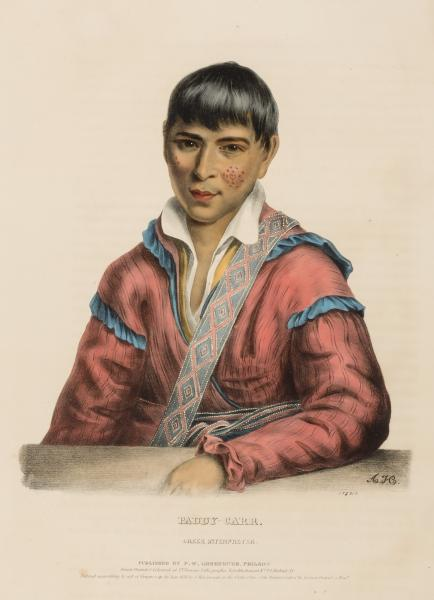
\includegraphics{images/0202b_images/image1.jpg}
\caption{alt\_text}
\end{figure}

\url{https://drive.google.com/open?id=1OvngfWlXkBOrMQyUwMzWSniiC5CxKiNe}

We even have a beautiful portrait of the second Paddy Carr, from the Smithsonian's National Portrait Gallery, done by Alfred M. Hoffy in 1838.

More information about this second Paddy Carr is in McKenney and Hall (1838, p 223-225). It documents his trip as interpreter to Washington, his subsequent career as a trader, slaveholder, and landed gentleman, and his leading of 500 warriors in the Florida campaign.

\begin{quote}
\emph{The young Paddy was born near Fort Mitchell, in Alabama, and, in his infancy, was taken into the family of Colonel Crowell, the Indian agent, and kindly reared in the habits of civilised life (p 223).}
\end{quote}

\begin{quote}
\emph{Soon after his return from Washington, he married the daughter of Colonel Lovett, a respectable half breed, with whom he received a portion which, with the property accumulated by himself, furnished a capital sufficient to enable him to go into trade. In a few years he amassed a considerable property, and is now, in 1837, possessed of from seventy to eighty slaves, besides landed property, and a large stock of horses and cattle. (p 223)}
\end{quote}

\begin{quote}
\emph{Paddy Carr has an innate passion for fine horses, and owns a large number of very valuable animals. He is fond of racing, and, when he has a trial of speed depending, if he cannot suit himself with a rider, he rides his own horse. He is of a liberal and generous disposition, hospitable to strangers, and kind to the poor. Many of the poorer class of Indians depend on him for support. He has three wives, one of whom is daughter of the ill fated General McIntosh. The two first born of his children were twin girls, and Captain Crowell, the son of his early friend and patron, having a daughter named Ariadne, he called one of his twins Ari and the other Adne, thus evincing a sense of benefits received, which is in itself one of the highest evidences of a noble mind. (p 224)}
\end{quote}

Enough of Paddy Carr, and back to the main characters of this chapter.

\hypertarget{life-and-death}{%
\subsection{Life and Death}\label{life-and-death}}

The book by Alley (1885, p.~381) has a short biographical sketch describing David Ulery. I assume Alley actually talked to Ulery, because his book was ``\emph{compiled from the most authentic sources}''.

\begin{quote}
\emph{The subject of this sketch was born in Fayette county, Pennsylvania, May 11, 1831, but when fifteen years of age removed to Wheeling, Ohio county, West Virginia, where he was engaged in steamboating. He afterwards joined his parents in Muscatine county, Iowa, and subsequently moved to Minneapolis, and thence to Crawford county, Wisconsin, and there was married to Miss Martha J. Alcorn. In the spring of 1861 he emigrated to California via the isthmus of Panama, and after remaining in Sacramento until July of that year he came to Portland, Oregon, settled on the road between that city and Vancouver and engaged in fruit and vegetable raising for the Portland market. Disposing of that place in 1882, he took up his residence in Clark county, Washington Territory, and in the month of March took possession of the farm he now occupies in the Chelachie valley. His family consists of one son and three daughters, viz.~John H., Mary, Rosa and Lena.}
\end{quote}

Note that Ulery bought the farm one month after receiving 1050 + 1200 + 1200 + 2500 + 700 = 6650 dollars from the sale of his donation land claim in Multnomah County. I am pretty sure that was quite a lot more than he paid A-Chars-War-Chee for the patent.

While living on Vancouver road, David Ulery was active in various public-minded activities. He served on juries and councils, and interacted with his neighbors Evander Howe, John Hotts, William Love, George Smith, and Lewis Love, all of them featuring in various chapters of this book. If appraisals were needed, or documents signings needed to be witnessed, then the neighbors helped each other, undoubtedly also because they were the only people around, living in an isolated area, far from the city. In the Willamette Farmer of March 7, 1874, we see Ulery as active in the Grange movement ``\emph{a fraternal organization in the United States that encourages families to band together to promote the economic and political well-being of the community and agriculture}'' (Wikipedia). It's like a rural neighborhood association.

\begin{figure}
\centering
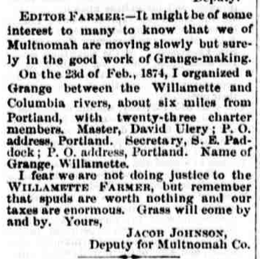
\includegraphics{images/0202b_images/image2.png}
\caption{alt\_text}
\end{figure}

We can also follow David Ulery through the pages of the federal and state censuses.

\url{https://drive.google.com/open?id=1U8VH0G83sIc_dwDzT9OUADiaEczNtpy2}

In 1850 he was 19 years old, living with his parents in Marshall county, Virginia. His profession was listed as cooper. His future wife Martha Jane Alcorn was 14, and living with her parents in Kiskiminetas, Armstrong, Pennsylvania. In 1870 Ulery was a farmer in the Willamette precinct, Multnomah county, owning \$ 2,500 worth of real estate, and accompanied by his wife and children John (12) , Mary (8), Rosa (7), Benj (4) and Lisor Ann (2). In the 1880 federal census Rosa Ann (16), Benjamin (14), and Lissa (12) are still at home. In the 1900 federal census the children are not there anymore, and husband and wife are in Chelatchie county in Washington. They are by now 69 and 64 years old, and the census informs us that of their six children only three are still alive. In the 1910 census David and Martha are 76 and 74. After that, no more.

\begin{figure}
\centering

\includegraphics{images/0202b_images/image3.png}
\caption{alt\_text}
\end{figure}

The records of the Chelatchi Cemetery in Amboy, Washington (established 1892) show

\begin{figure}
\centering
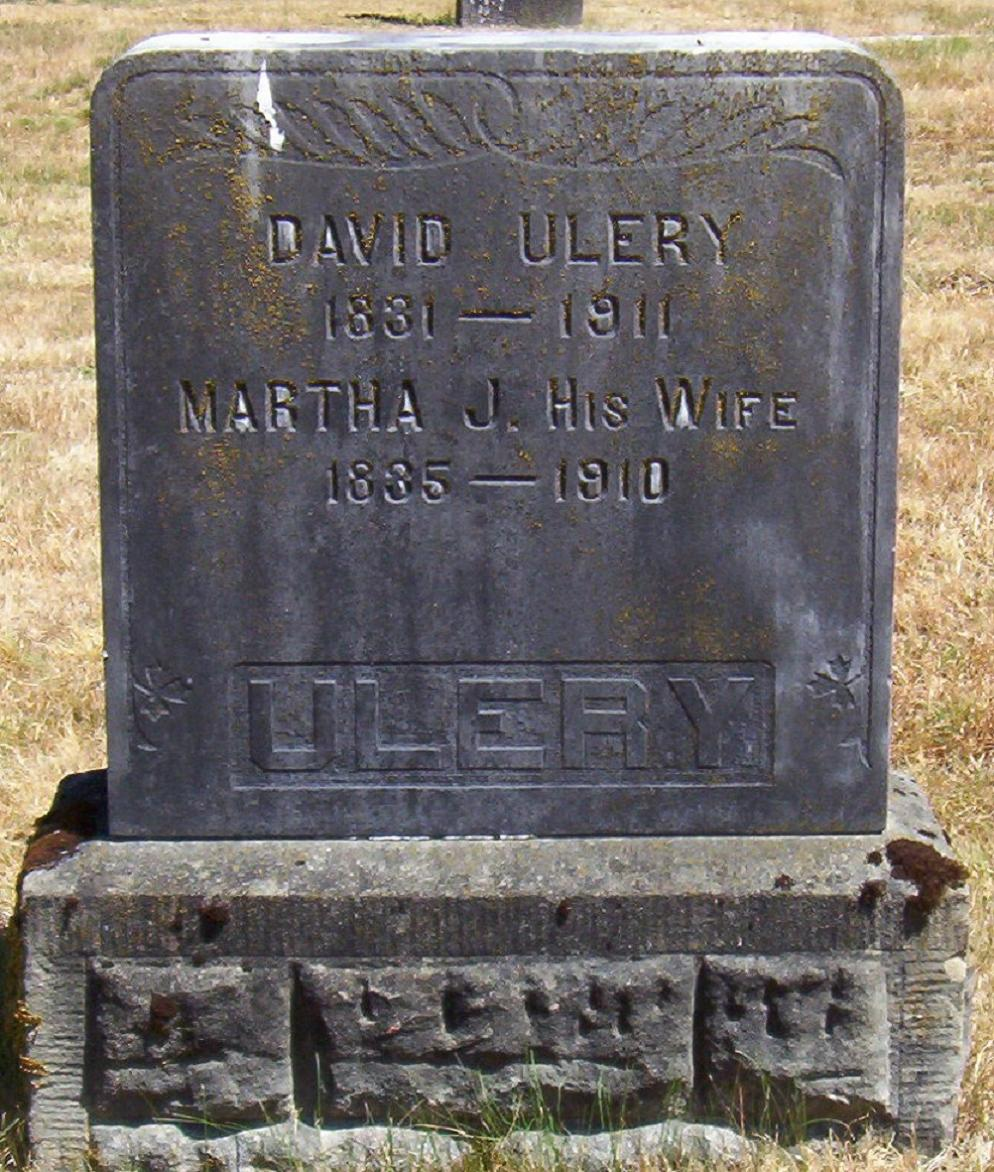
\includegraphics{images/0202b_images/image4.jpg}
\caption{alt\_text}
\end{figure}

\hypertarget{references-4}{%
\subsection{References}\label{references-4}}

Michael J. O'Brien: \emph{Major Patrick Carr and Captain Patrice McGriff, two Gallant Officers of the Georgia Continental Line}. The Journal of the American Irish Historical Society, 21, 1922, 97-102 \url{https://drive.google.com/open?id=1BEmLmHzPeLPdpwkf1KNnxosi9Wvbo0Zc}

Thoma L. McKenney and James Hall: \_Biographical Sketches and Anecdotes of Ninety-Five of 120 Principal Chiefs from the Indian Tribes of North America. \_United States Department of the Interior, Bureau of Indian Affairs, Report 432, 1838 \url{https://drive.google.com/open?id=1POMHnkh4sljQSywARyBrYFlMW20R7twL}

Wikipedia, \emph{Creek War }\url{https://en.wikipedia.org/wiki/Creek_War}

Wikipedia, \emph{Creek War of 1836. \url{https://en.wikipedia.org/wiki/Creek_War_of_1836}}

Wikipedia, National Grange of the Order of Patrons of Husbandry \url{https://en.wikipedia.org/wiki/National_Grange_of_the_Order_of_Patrons_of_Husbandry}

Federal and Washington State Census Records 1850-1910 \url{https://drive.google.com/open?id=1U8VH0G83sIc_dwDzT9OUADiaEczNtpy2}

B. F. Alley: \_History of Clarke County, Washington Territory, Compiled from the most Authentic Sources. Also Biographical Sketches of its Pioneers and Prominent Citizens. \_Washington Publishing Company, Portland, Oregon, 1885 \url{https://drive.google.com/open?id=1lSH0vBcrdK2gx7btAFHorsPdnZ1rgm2e}

\hypertarget{homesteads-george-and-elizabeth-smith}{%
\section{Homesteads: George and Elizabeth Smith}\label{homesteads-george-and-elizabeth-smith}}

\begin{figure}
\centering
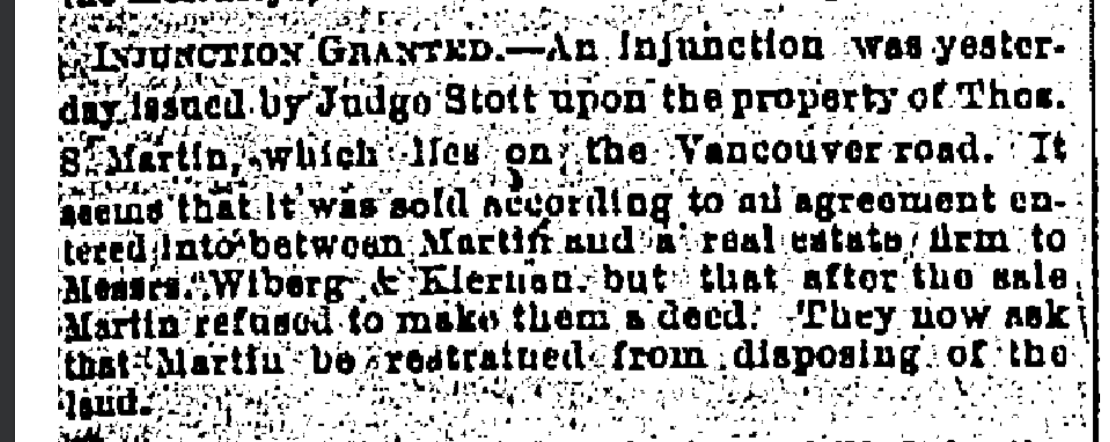
\includegraphics{images/0203a_images/image1.png}
\caption{alt\_text}
\end{figure}

\hypertarget{homestead-2}{%
\subsection{Homestead}\label{homestead-2}}

\begin{figure}
\centering
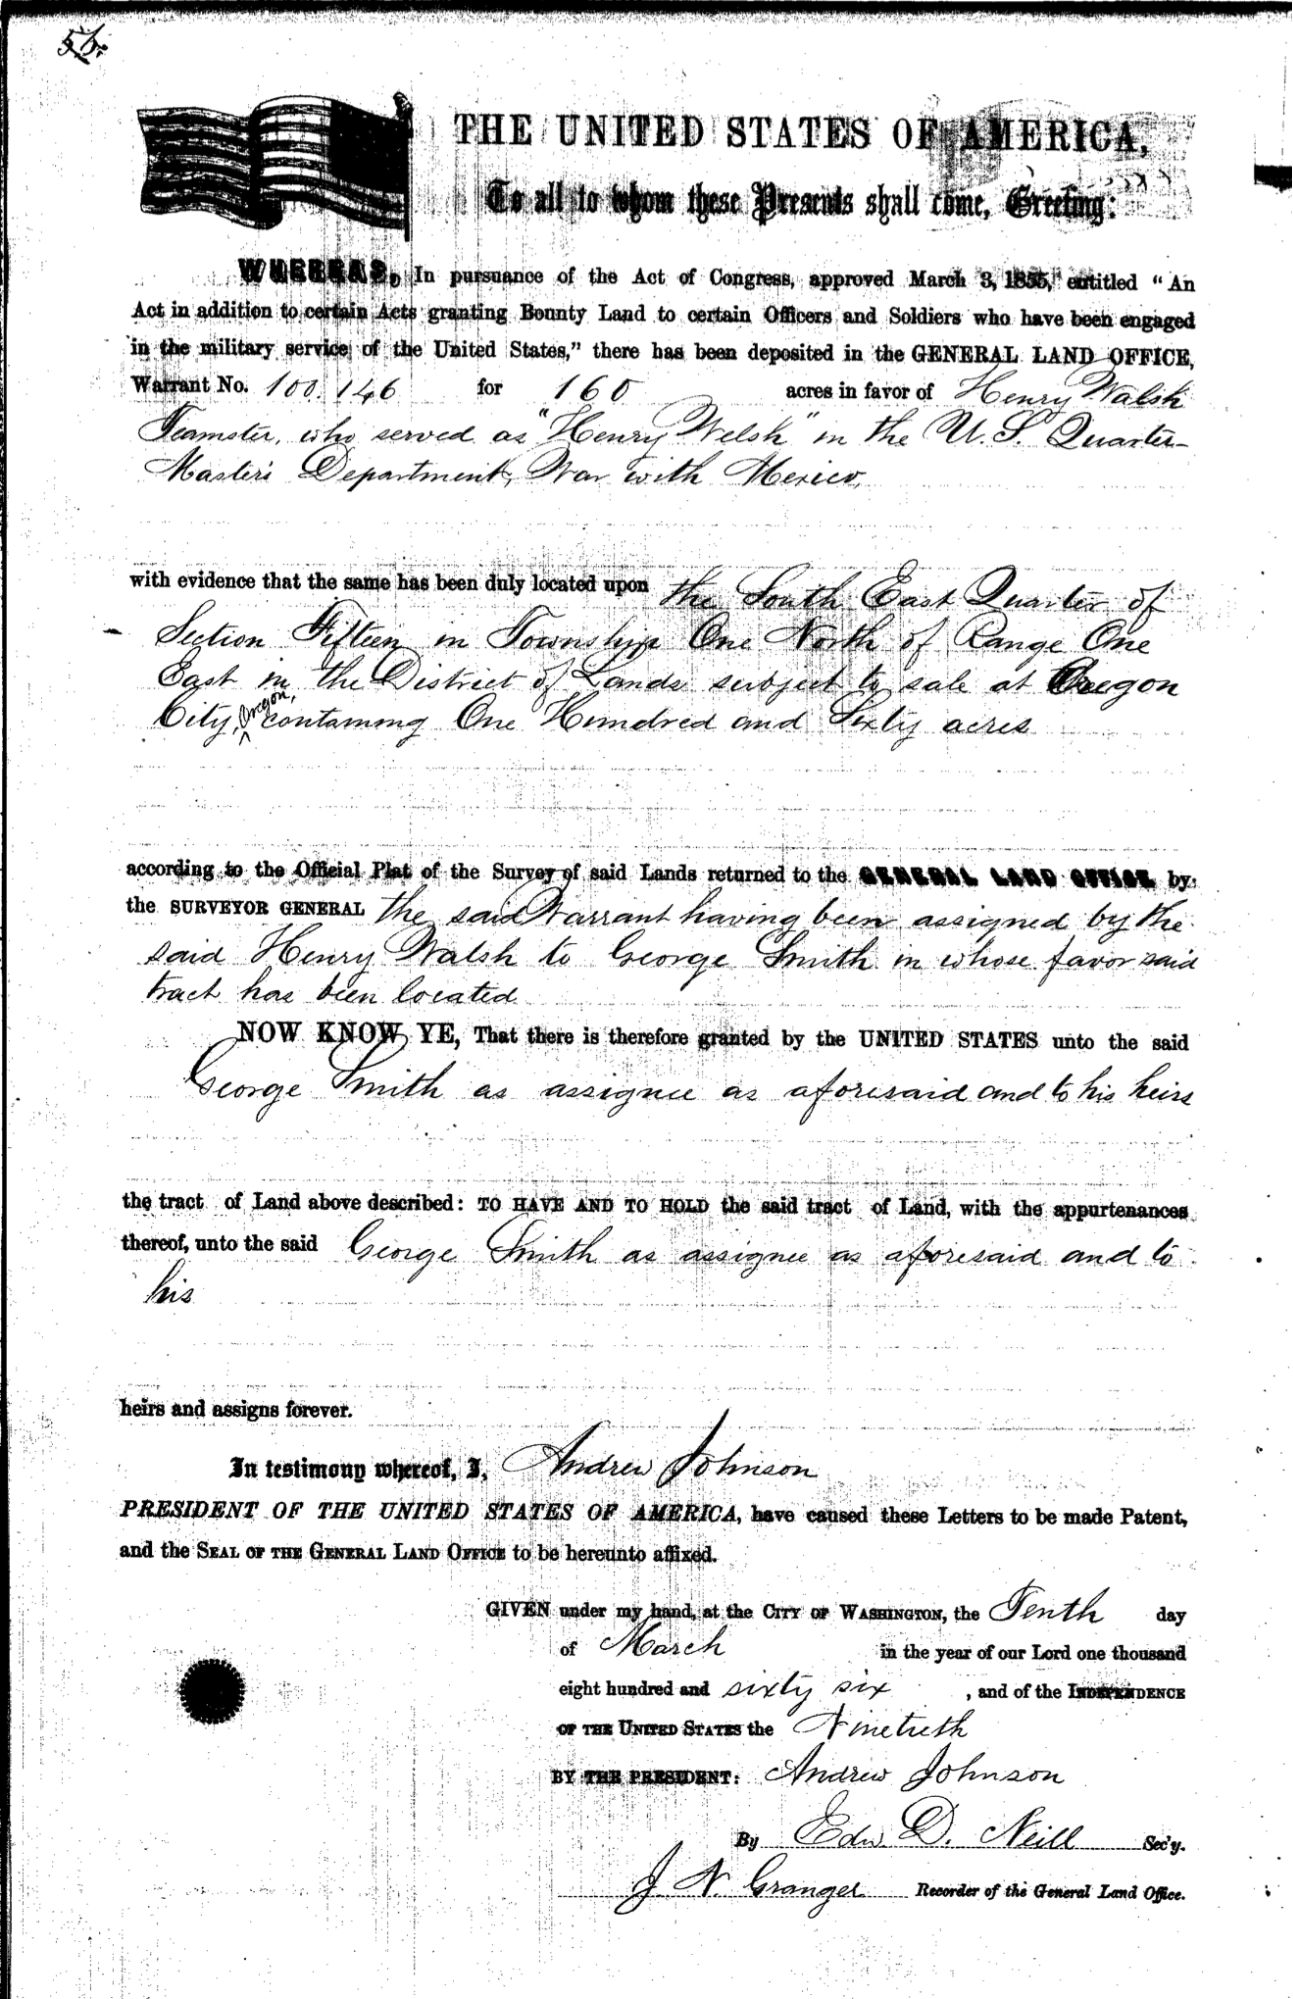
\includegraphics{images/0203a_images/image2.png}
\caption{alt\_text}
\end{figure}

\url{https://drive.google.com/open?id=0B94Urj3OjM7Bd0RRSjFMcnp3Ulk}

On March 10, 1866 the United States donated 160 acres, using the Military Donation act, to Henry Walsh, for his service as teamster in the US Quartermaster's Department in the War with Mexico. Henry Walsh immediately transferred the land to George Smith. The description of this track of land is simple: the southeast quarter of section 15, township one north, range one east. The corresponding deed was recorded with Multnomah County on June 22, 1870.

\url{https://drive.google.com/open?id=1AERgX2cBf44CjtJ608IxXLA0rYUVPAQB}

To the west of the land now owned by George Smith was the homestead of Evander Howe, another 160 acres, the southwest quarter of section 15, township one north, range one east. As I have documented in the chapter on Evander Howe he sold the southern eighty acres of his tract on July, 5 1870 for four hundred dollars to Elizabeth Smith, George Smith's wife. In other words, at that time George and Elizabeth owned 240 acres. That is the area in the blue boundary on the first page of this chapter.

\hypertarget{sales-1}{%
\subsection{Sales}\label{sales-1}}

Eventually, in 1888, George Smith's donation land ended up with Edward Quackenbush's Investment Company. It was platted to become the Piedmont subdivision. But before that it changed hands many times. This is a common and unavoidable phenomenon. Lands get partitioned by inheritance or sales, and the units get smaller and smaller. The price of land goes up and sales of smaller pieces remain economically viable. The history section of the Piedmont Neighborhood Plan (Portland Bureau of Planning, 1993, page 13) says

\begin{quote}
\emph{The quarter section of land which later became Piedmont was granted to Henry Walsh by the United States Government on March 10, 1866. Pursuant to an 1855 act of Congress, this land was a Bounty Land Claim for his military service in the Mexican-American War. After changing hands several times between 1870 and 1888 with many legal questions over ownership, the entire parcel was sold for \$ 24,000 to the Investment Company on June 22, 1888.}
\end{quote}

This is a nice compact summary, and it even is mostly correct, but there is not enough detail for my purposes. It does not even mention George Smith, and the alleged legal questions are interesting. So I have filled in the details. To some this may appear tedious, but it was a lot of work and it seems useful to document it once and for all.

On August 2, 1870 George and Elizabeth Smith sold their 240 acres for \$ 2,400 to H.F. Bloch and A.P. Dennison. Note that they recorded the deed to their 160 acres in June 1870, and they added the 80 acres of Evander Howe in July 1870. They moved quick.

\url{https://drive.google.com/open?id=1PrnthO0q74hsYLIL4BryA5t0xg84IstH}

Bloch and Dennison, who we will talk about a bit more in another chapter of this book, also used the land for speculative purposes only. They quickly sold it as well, in three pieces.

On January 12, 1872 to P.J. Smith and C.H. Burrage for \$ 1,250, the southwest quarter of the southwest quarter of section 15, 40 acres.

\url{https://drive.google.com/open?id=1SpPjBuKXLwY_xzwj2n5JEV5HBprK1APU}

On January 31, 1872 to Isaac Dillon for \$ 1,250, the southeast quarter of the southwest quarter of section 15, 40 acres.

\url{https://drive.google.com/open?id=1T3nOZezPJA-7KUNX8QLEy2KCWF35QFJ4}

On February 26, 1872 to P. J. Martin and D. F. Harrington for \$ 5,000, the southeast quarter of section 15, 160 acres.

\url{https://drive.google.com/open?id=1T4CsSZM13xThPJCuBKasscWgOf98NqBZ}

Note that the southern half of Evander Howe's homestead claim is not in the modern Piedmont neighborhood, so I will not further follow the title chains for that piece of land. At least not for now. Eventually that half will host the subdivisions West Piedmont, North Albina, and Jarrett's Addition.

After Bloch and Dennison sold there were various complications with sales of the southeast quarter of section 15, the original George Smith claim, mostly because of internal problems in the Edward Martin family empire, which are discussed in detail in our P.J. Martin chapter. For our purposes here it is sufficient to know that around 1858 Edward Martin started, among other things, the wholesale liquor business E. Martin \& Co.~in San Francisco, partnering with D. V. B. Henarie, who ran the daily management of the firm. Edward's brother Patrick J. Martin, universally known as P. J. Martin, moved to Portland in 1868 and went into the real estate business here. Edward's sons, Thomas S. Martin and Edward Martin moved to Portland around 1880 to start a nominally independent Oregon liquor business with the same name. They did not do very well, however, and soon the Portland company was \$ 50,000 in debt to the San Francisco company. They went into receivership, and the assets of the Oregon company were subsequently bought by the San Francisco company. In 1880 Edward Martin Sr.~died and P. J. Martin moved back to San Francisco. Much more on the Martin family is in the chapter that discusses them in more detail. It is of interest that events in the Martin family are reflected in the real estate sales in Portland.

First, D. F. Harrington quitclaims, for \$ 1, his interest in the 160 acres to P. J. Martin on June 16, 1877. Note that Harrington, a member of Portland's Common Council (now the City Council), moved to San Francisco in 1877.

\url{https://drive.google.com/open?id=1N4hmqbWHuECF7OjmyULRPtPY1MCQkh59}

On February 14, 1881 P. J. Martin and Margaret A. Martin his wife quitclaim, for \$ 1, the 160 acres to their nephews Thomas S. Martin and Edward Martin.

\url{https://drive.google.com/file/d/1RtBq1Y2S3U-mi75Wis5LmEshP5JkYTcL/view}

On July 12, 1881 P. J. Martin and Margaret A. Martin his wife use a warranty deed for \$ 5 to grant the 160 acres of George Smith's DLC to Thomas S. Martin and Edward Martin, together with other pieces of land in Clackamas and Marion counties.

\url{https://drive.google.com/file/d/1RuH3FA4Gx5Z5QTQsUt1N0KX1aC_rt4xv/view}

These two last quitclaims are at the time that Thomas and Edward moved to Oregon after the death of their father. Presumably they were his legal heirs. At the time Thomas was 27, and Edward was 25. Pretty quickly, however, their fortunes went south. Literally.

In the Oregonian of April 19, 1882 we see the first sign of trouble with the ownership of Edward Jr.~and, especially, Thomas Martin.

\begin{figure}
\centering
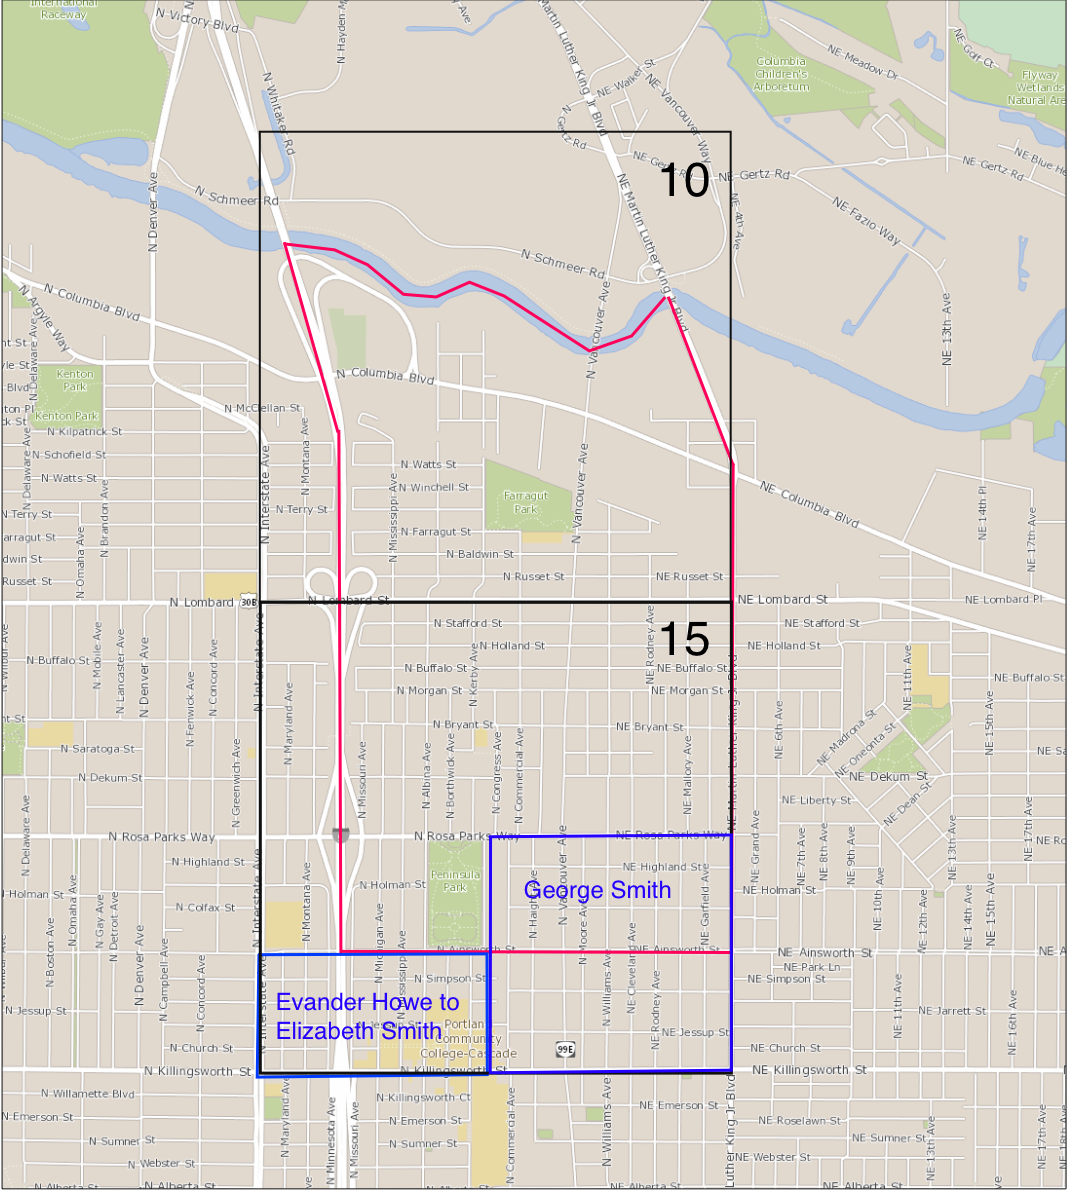
\includegraphics{images/0203a_images/image3.png}
\caption{alt\_text}
\end{figure}

The Portland branch of E. Martin \& Co.~was getting into trouble. On April 10, 1883 Edward Martin granted Power of Attorney to his uncle P. J. Martin.

\url{https://drive.google.com/open?id=1xANQ1n1yvlb1jMgQfrHH5u3sXKHn5HlF}

This was at the same time that the company was entered into receivership, and a receiver was appointed to sell off the assets.

Then, on April 10, 1883, Thomas S. Martin and Edward Martin sold the 160 acres to Daniel V. B. Henarie for \$ 40,000.

\url{https://drive.google.com/open?id=1IKrgbQykJurwWGCuvgRF51zu25uekfDG}

That seems to be too much money. But remember that E. Martin \& Co.~of Portland still owed to E. Martin \& Co.~of San Francisco, controlled by Henarie, more than \$ 25,000. This may have been one way in which the delinquent brothers were helped to pay off their debts.

On February 12, 1884 Thomas S. Martin and Ada B. Martin his wife sold their interest in the 160 acres, together with substantial parcels of land in Clackamas, Marion, Wasco, and Baker county to Edward Martin for \$ 4,000.

\url{https://drive.google.com/open?id=1ELF2NrYzc3LoVIwAbLJLKXINnMtwX4qj}

An article from the Morning Oregonian of May 9, 1888, included below, indicates that he got rid of his title and interest in E. Martin \& Co.~around the same time. It is interesting that people quitclaim parcels to which they do not have clear and free title. Although it largely stays in the family.

Edward L. Dorn would have none of it. There is a deed from February 2, 1888 in which Thomas A. Jordan, Sheriff of the County of Multnomah, grants the 160 acres of the Smith claim to E. L. Dorn.

\url{https://drive.google.com/open?id=1Z6myupQds23-rOQAo80rPbrn1pDUFUae}

I'll transcribe this deed, complete with all its legal jargon, annoying repetitions, and lack of punctuation, because it is different from others in this book, and because it documents what happened at this point in time to Edward Martin and the Smith grant. Also, Sheriff's deeds are inherently more complicated than general warranty deeds or quitclaim deeds, and give more information about the actual historical situation. This one shows how sons of millionaires can get into trouble, even if other millionaires are trying to bail them out.

\begin{quote}
\emph{This indenture, made the second day of February, in the year of our Lord one thousand eight hundred and eighty eight, between Thomas A. Jordan, Sheriff of the County of Multnomah, the party of the first part, and E. L. Dorn, the part of the second part, witnesseth. That whereas by virtue of a writ of Execution and Order of Sale issued out of and under the seal of the Circuit Court of the State of Oregon for the County of Multnomah, dated the 28th day of March, A. D. 1887, upon a judgment docketed in the said Court on the 26th day of March, 1887, in favor of R. D. Freeborn, plaintiff and against Edward Martin, defendant, to the said Sheriff directed and delivered, commanding him that, out of the personal property of the said judgment debtor in his County, he should cause to be made some money in the said write specified, and if sufficient property of the said judgment debtor could not be found, then he should cause the amount of the said judgment to be made out of the real property belonging to said judgment debtor on the 26th day of March, A.D. 1887, or at any time afterward. And, whereas, because sufficient property of said judgment debtor could not be found, whereof the said Sheriff could cause to be made moneys specified in said writ, the said Sheriff did, on the fourth day of April, A.D. 1887, in obedience to said command, levy on, take and seize all the right, title, interest and claim which the said judgment debtor so had to the lands, tenements, real estate and premises hereinafter particularly set forth and described, with the appurtenances, and did on the ninth day of May, A.D. 1887, sell all the right, title, interest and claim of the sad judgment debtor in and to the said premises at public auction, in front of the Court House, in the City of Portland, in said County of Multnomah, between the hours of nine in the morning and four in the afternoon of that day namely: at 10 o'clock, A.M. after first having given due notice of the time and place of such sale, according to law, to wit: By posting notice of the time and place of sale, particularly describing the property for four weeks successively prior to the date of sale, in three of the most public places, in the County of Multnomah, and also by publishing a copy of such notices once each week for four successive weeks prior to said date of sale in the Sunday Welcome, a weekly newspaper of general circulation, printed and published in Multnomah County, State of Oregon, at which sale all the right, title, interest and claim of the said judgment debtor in and to the said premises were struck off and sold to the said R.D. Freeborn, for the sum of two hundred and forty five dollars, lawful money of the United States of America, the said R.D. Freeborn being the highest bidder, and that being the highest sum bid for the same, whereupon the said Sheriff , after receiving from the said purchaser the said sum of money so bid aforesaid, gave to the said purchaser such certificate of sale as is by law directed to be given, and the matters contained in such a certificate were substantially stated in said Sheriff's return of his proceedings upon said write to the County Clerk of the said County of Multnomah. And, whereas, the said Court by an order dated the 10th day of September 1887 confirmed said sale and four months have expired since the confirmation of said sale by said Court without any redemption of the said premises having been made: and whereas by an assignment duly made upon said certificate the said R.D. Freeborn has duly transferred all right therein to the party of the second part. Now this indenture witnesseth that the said Thomas A. Jordan, the Sheriff aforesaid, by virtue of the said writ, and in pursuance of the Statute in such case made and provided, for and in consideration of the said sum of money, to him in hand paid, as aforesaid, by the said party of the second part, the receipt whereof is hereby acknowledged, has granted, bargained, sold, conveyed, and confirmed, and by these presents does grant, bargain, sell, convey, and confirm unto the said party of the second part and to his heirs and assigns forever, all the right, title, interest, and claim which the said judgment debtor Edward Martin had on the said fourth day of April, A.D. 1887, or at any time afterwards, or now has, in and to all that certain lot, piece or parcel of land, situated, lying and being in the said County of Multnomah, State of Oregon, and bounded and particularly described as follows, to wit: The South East quarter of section fifteen in township one North range one East of the Willamette Meridian. Together with all and singular the hereditaments and appurtenances thereunto belonging or in any wise appertaining. To have and to hold the said premises with the appurtenances, unto the said party of the second part, his heirs and assign forever, as fully and absolutely as the said Sheriff can, may, or ought to, by virtue of the said writ and of the statute in such case made and provided, grant, bargain, sell, convey and confirm the same. In witness whereof the said Sheriff, the said party of the first part, has hereunto set his hand and seal, the day and year first above written.}
\end{quote}

Remember, however, that Daniel B. V. Henarie paid Thomas and Edward Martin \$ 40,000 for the land, and that Thomas subsequently quitclaimed his interests to Edward. Thus there was no clear title for E. L. Dorn, although he legally obtained Edward Martin's interests for \$ 245 from R. D. Freeborn, who won them during the Sheriff's sale. The court had to settle that the quitclaim for \$ 40,000 was actually a mortgage on the property to pay off the debt, and that Edward Martin consequently had a clear title.

\begin{figure}
\centering
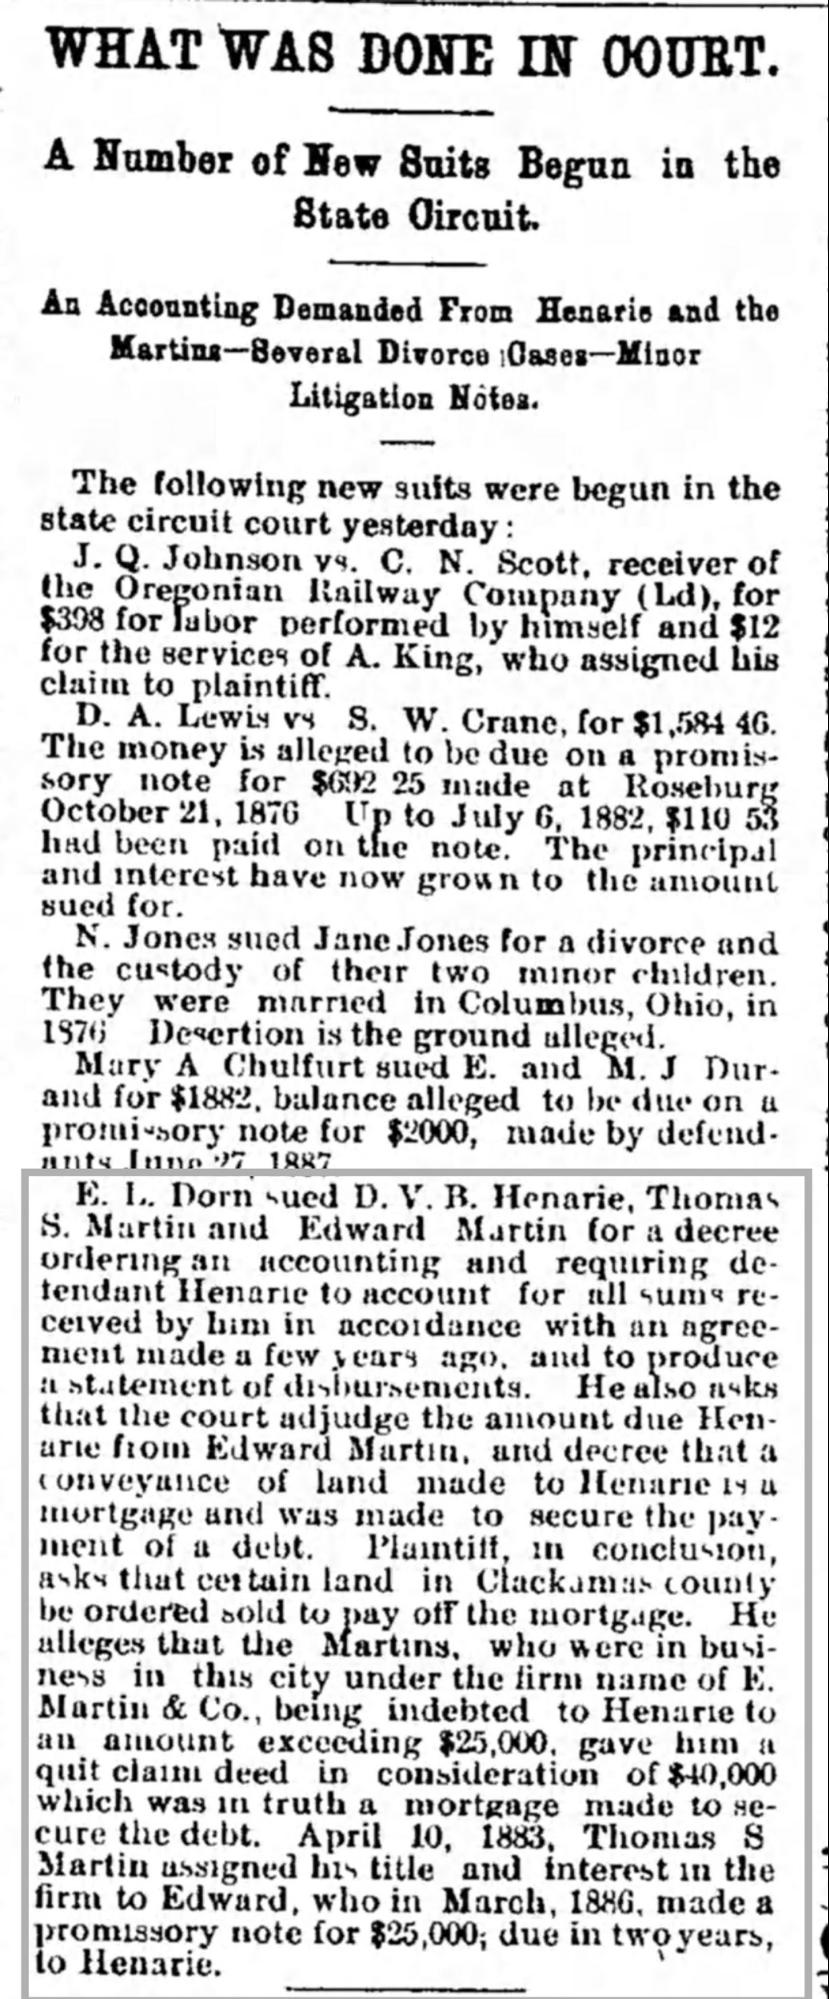
\includegraphics{images/0203a_images/image4.jpg}
\caption{alt\_text}
\end{figure}

It is unclear how the court case ended, and if Dorn got his land in Clackamas County (320 acres, by the way). Probably. In May 26, 1888 E. L. Dorn and Kate Orr Dorn his wife quitclaimed the Smith grant of 160 acres to the Investment Company for \$ 1.

\url{https://drive.google.com/open?id=1SizrqEp901cz4Pdn97HEpMl-y5TInobm}

Edward Martin was involved in one last sale of the property. One June 1, 1888 there is a warranty deed from Edward Martin to Charles A. Neal for \$ 1,500.

\url{https://drive.google.com/open?id=1rNYlyJ9DI1VtsBgHddZ5FVp8kxt0zaUu}

The deed has the usual language, but says:

\begin{quote}
\emph{And I, the grantor above named, do covenant to and with the said Chas. A. Neal, the above named grantee, his heirs and assigns, that the above granted premises are free from all encumbrances made, executed, or suffered by said grantor, save a conveyance of the same to D.V.B. Henarie, made or intended as a mortgage, recorded on page 368 of book 66 of the records of deeds of said County, and that I will and my heirs, executors, and administrators shall warrant and forever defend the above granted premises, and every part and parcel thereof against the lawful claims and demands of all persons whomsoever, claiming or to claim the same by, from, through or under the said grantor.}
\end{quote}

For \$ 1,500 Edward Martin was out of the picture. The next step is a deed of June 2, 1888 from D. V. B. Henarie to Charles A. Neal for \$ 24,000.

\url{https://drive.google.com/open?id=1E2zdE1VlfCVA49PHvge9IaFZz82BIZdk}

It says:

\begin{quote}
\emph{The object of this conveyance is to discharge and release the said real estate from the lien and encumbrances thereupon created by operation of the deed from Thomas S. Martin and Edward Martin to me, recorded upon the records of deeds of Multnomah County, State of Oregon, on page 368 of book 66, the same having been made and intended as a mortgage and to satisfy and discharge a judgment lien docketed in the judgment lien docket of said County and State on Oct.~6 1886, against said Edward Martin for \$ 2569.92.}
\end{quote}

And now, finally, with all of the Martins no longer involved, on June 26, 1888 Charles A. Neal, deeds the Smith claim for \$ 24,000 to the Investment Company.

\url{https://drive.google.com/open?id=1Sh2UmtFNRpZD-THByooAPiQ_7ME5dDEu}

The next year the development of Piedmont started.

\hypertarget{homesteaders-george-and-elizabeth-smith}{%
\section{Homesteaders: George and Elizabeth Smith}\label{homesteaders-george-and-elizabeth-smith}}

\hypertarget{life-1}{%
\subsection{Life}\label{life-1}}

As explained earlier the military donation claim of Henry Walsh in 1866 was immediately transferred to George Smith. The claim was recorded in June 1870, but in the same year George and his wife Elizabeth sold all their property in Multnomah County. Snyder (1989, p.232) has no personal information about George and his wife Elizabeth Smith, only the dates from the deeds. I will try to come up with more, but for now it will be tentative.

Clearly George and Elizabeth Smith did not stay very long in the Piedmont real estate limelight, basically only for a few months in 1870. I have not been able so far to find any definite information about them in the local papers or in the census and the usual ancestry sources. One problem I also mention in the chapter on Liverpool Liz is that there are just too damn many Smiths, and even too many George and Elizabeth Smith pairs. It is difficult to tell them apart without information about birth, death, or place of residence.

For a moment I thought that maybe this Elizabeth Smith was actually the same person as Liverpool Liz, who was of course also an Elizabeth Smith (among other things). But I am pretty sure Liverpool Liz was born around 1860, and it is unlikely she would have bought the 80 acres from Evander Howe when she was 10 years old. At that time she was probably still playing with her sailor dolls on the other side of the Atlantic.

I do have one hypothesis, however. It is somewhat wild and unsupported, but I'll continue to test it. The idea is that the homesteaders in our area were all farmers and neighbors on Vancouver Road, on or just south of the Columbia Slough, in the Willamette Precinct. Lewis Love, William Love, Evander Howe, John Hotts, John Rankin, and David Ulery all lived in that area. Only John Fenstermacher did not, but he sold the homestead he acquired in the Willamette precinct immediately to John Hotts. When William Love died in 1878 and an administrator had to be appointed for the estate, the appraisers were David Ulery and John Hotts. When John Rankin's wife died in 1860 and a guardian had to be appointed in 1871 for the heirs who were still minors, the appraisers of the estate were William Love, David Ulery, and John Hotts. Seems a pretty close knit group of neighbors to me. Or, to give it a slightly different emphasis, nobody else lived anywhere near.

The 1870 federal census for the Willamette precinct shows David Ulery and John Hotts as census neighbors, meaning that their homes were visited by the census person directly after each other. Another census neighbor was G. A. Smith, a 26 year old farmer, owner of land valued at \$ 4,000. That is George Aaron Smith. His wife Elizabeth was 21, and his children Caroline (5), Rosetta (3), and Charles (1) lived at home.

\url{https://drive.google.com/open?id=1UIogLrnVAXkM8sVKXJcR3YxfC4tV2YHi}

Some further research shows that Elizabeth's maiden name was Rankin, and that she was the oldest daughter of John Rankin, a neighbor to the east of Vancouver Road. She was born March 28, 1849, ad she married George Smith in 1863, when she was 14. In the 1880 federal census we do no longer see the Smith's in Willamette precinct, but Hotts and Ulery are still there.

\url{https://drive.google.com/open?id=1UG_QRBABD8gPf79ShC7yWP__qr3oubIK}

In fact, by 1880 George and Elizabeth had moved to Chinokville, Pacific County, Washington, across the river.

\url{https://drive.google.com/open?id=1UU2IgfGrWXRdtqwK6oOjGDbCDP8moWW0}

Everybody now is ten years older, and they have been joined by offspring Louise (8), George (5), Ellen (3), and John (1). In the 1900 and 1920 census the Smith family had moved to Camas Valley in Douglas County, Oregon.

\begin{figure}
\centering
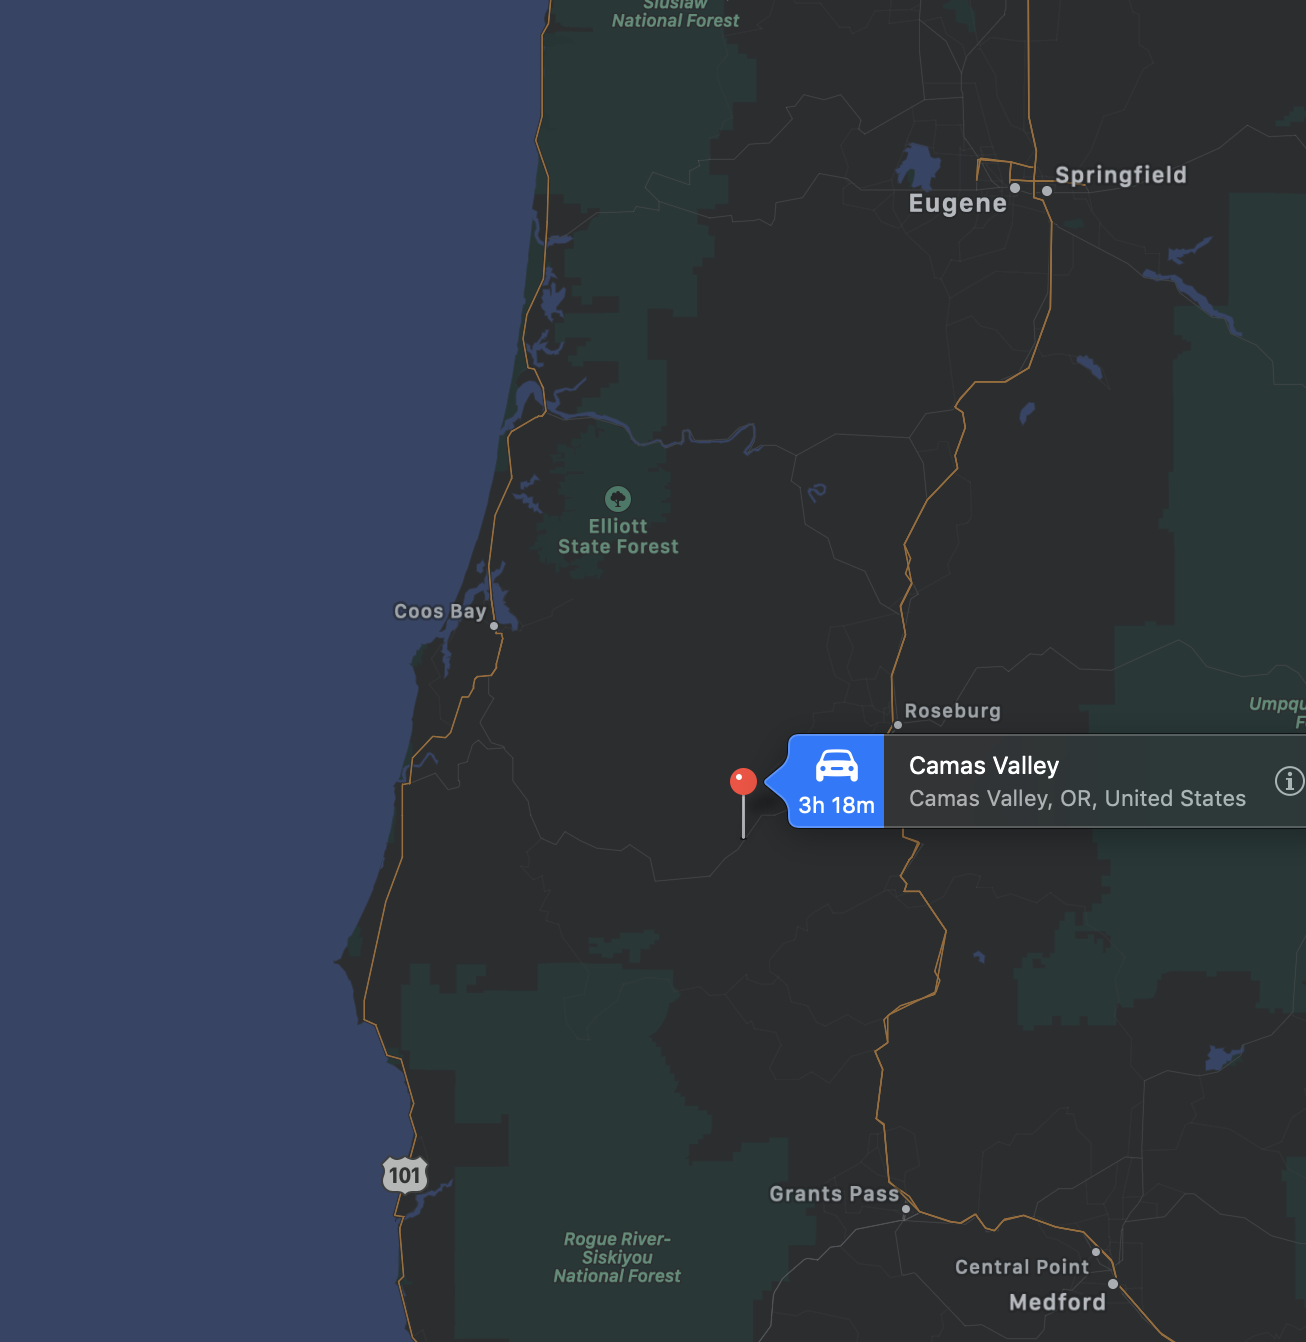
\includegraphics{images/0203b_images/image1.png}
\caption{alt\_text}
\end{figure}

To get a somewhat clearer picture of the numerous offspring I made a little table with ages in the various census records. In 1860 Elizabeth still lives with her parents, in 1870 and 1880 the family lives in Chinokville, and in 1900 and 1920 in Camas Valley. George Smith died in 1915, Elizabeth on October 14, 1925. They were both buried in the Murray Cemetery in Camas Valley.

1860

1870

1880

1900

1920

George A.

36

46

65

Elizabeth

11

21

31

51

70

Caroline E.

5

14

Rosetta M.

3

12

Charles W.

1

11

31

50

Louise

8

George

5

Ellen

3

John

1

David

18

Frank B.

15

32

Roseanna

13

My hypothesis is that this George Aaron Smith and this Elizabeth Rankin Smith were the ones who acquired Henry Walsh's bounty claim and Evander Howe's homestead, and subsequently sold it to Bloch and Dennison. They did have enough money to buy the land, because Elizabeth sold her share of her mother's inheritance to her father for \$ 2,000. In the deeds, linked below, note that George does not use his middle name, so that the grantors are named as George Smith and Elizabeth Smith, his wife. The deeds are recorded 10/18/1866 and 10/7/1867, which is the same year George Smith obtained the donation land claim land from Henry Walsh.

\url{https://drive.google.com/open?id=19zKctuiu8d2cL95mnl4g5m6PmideYJEL}

\url{https://drive.google.com/open?id=1RZpk8x_zAPfMMV4olhiKeQKZh6CTRV3A}

As I said, the evidence that this George A. Smith and Elizabeth Rankin are actually the ones the obtained the DLC is circumstantial, but they did live in the area and they did come into some inherited money at the time.

\hypertarget{references-5}{%
\subsection{References}\label{references-5}}

Eugene E. Snyder (1989): \_We Claimed this Land. Portland's Pioneer Settlers. \_Binfort \& Mort Publishing, Portland, Oregon

Portland Bureau of Planning (1993). \emph{Adopted Piedmont Neighborhood Plan.}

\url{https://drive.google.com/open?id=0B94Urj3OjM7Bc0pMMDZpOWY0NEk}

\hypertarget{homesteads-john-fenstermacher}{%
\section{Homesteads: John Fenstermacher}\label{homesteads-john-fenstermacher}}

{\textgreater\textgreater\textgreater\textgreater\textgreater{} gd2md-html alert: inline image link here (to images/image1.png). Store image on your image server and adjust path/filename/extension if necessary. }(Back to top)(Next alert){\textgreater\textgreater\textgreater\textgreater\textgreater{} }

\begin{figure}
\centering
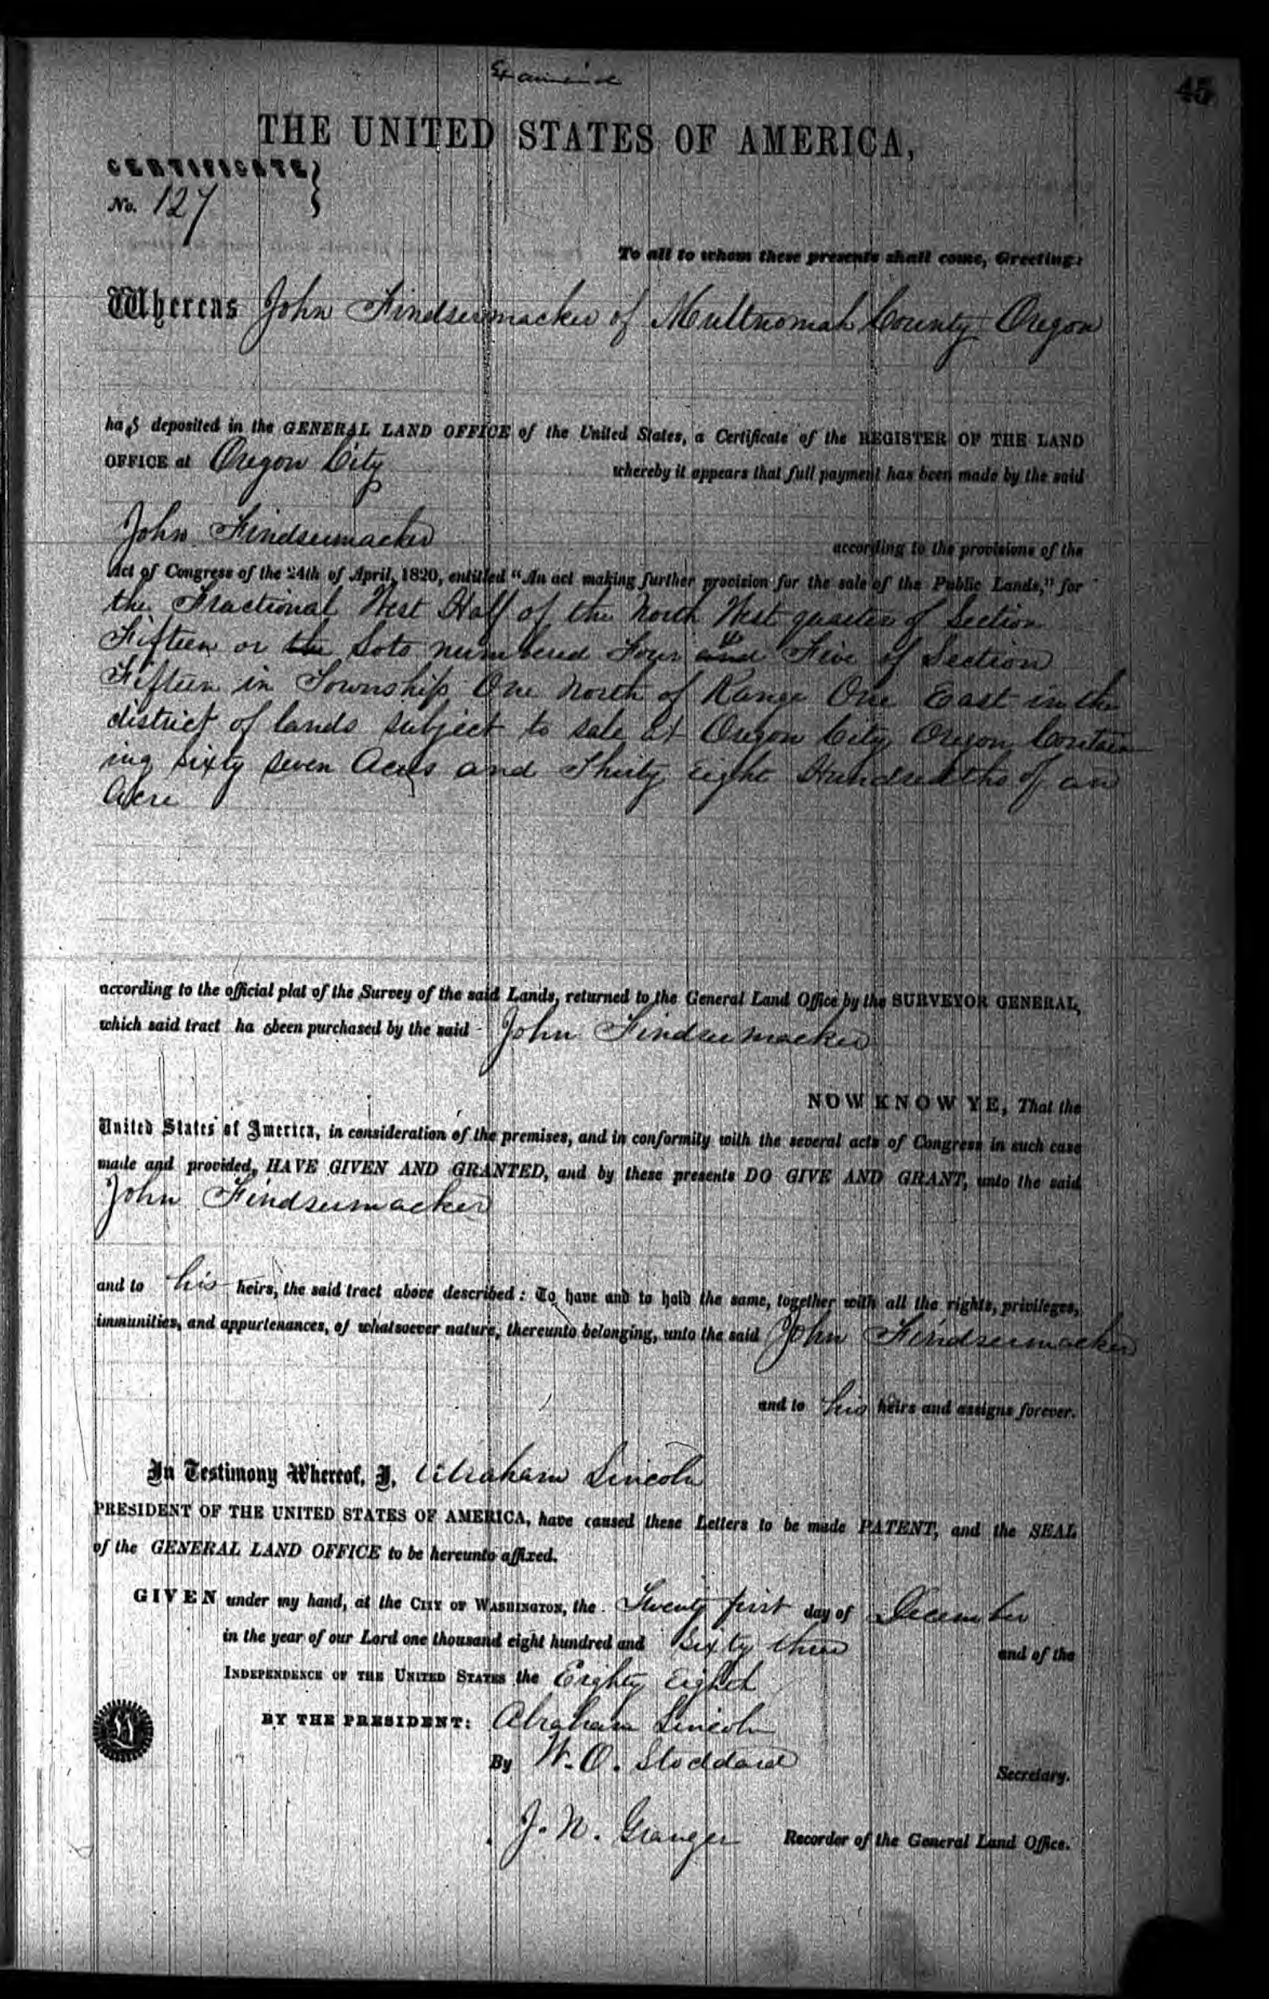
\includegraphics{images/0204a_images/image1.png}
\caption{alt\_text}
\end{figure}

\hypertarget{homestead-3}{%
\subsection{Homestead}\label{homestead-3}}

\begin{figure}
\centering
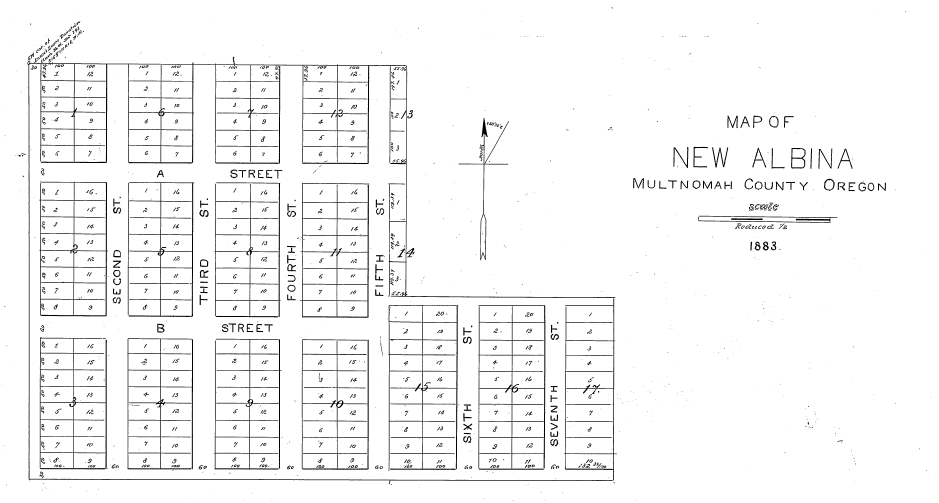
\includegraphics{images/0204a_images/image2.png}
\caption{alt\_text}
\end{figure}

\url{https://drive.google.com/file/d/0B94Urj3OjM7BczRxZlNjZmUtcFE}

On December 21, 1863 the United States registered the sale of 67.38 acres of public land for the usual \$ 1.25 per acre to John Findsermacker, under the provisions of the Act of Congress of the 34th of April, 1820, entitled \emph{``An act making further provision for the sale of public lands''}. For the moment, ignore the fact that the recipients name is spelled differently as the one in the title of this chapter.

The deed corresponding to the patent was not recorded with Multnomah County until January 17, 1880.

\url{https://drive.google.com/open?id=1pEM1Kkg_eau6sihj6llVo3_lHohzUKzL}

The precise description of the land is

\begin{quote}
\emph{The Fractional West Half of the North West quarter of Section Fifteen or the lots numbered Four and Five of Section Fifteen in Township One North of Range One East.}
\end{quote}

The following small map with donation claims and lot sales makes the description someone clearer.

\begin{figure}
\centering
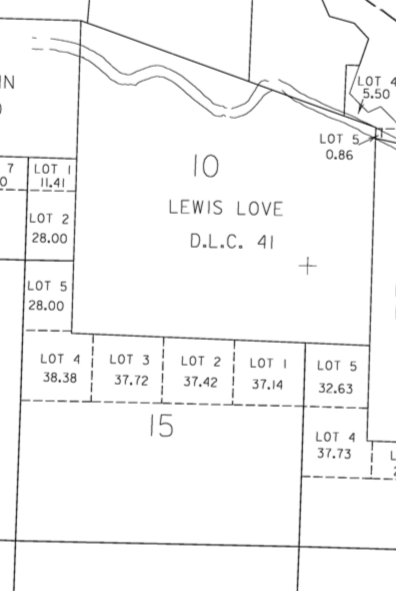
\includegraphics{images/0204a_images/image3.png}
\caption{alt\_text}
\end{figure}

Note that the west boundary of the Lewis Love DLC corresponds to what is now the I-5 freeway, while the south boundary is Bryant Street. Thus only a tiny sliver of Findsermacker's land is in modern Piedmont, only about the eastern third of lot 4, in fact about 14 acres. The rest is in modern Arbor Lodge. Also note that the map has an error, because the total acreage for lots 4 and 5 on the map is 28.00 + 38.38 = 66.38, while the patent specifies that Fenstermacher bought 67.38 acres. It looks as if the original intention was to make lot 4 equal to 20 chains by 20 chains, i.e.~a quarter mile by a quarter mile, or 40 acres.

In any case, he did not hold on to it for very long. Thus his role in the history of Piedmont is almost infinitesimal, but his life story is too interesting not to tell.

\hypertarget{sales-2}{%
\subsection{Sales}\label{sales-2}}

Fenstermacher sold his land on October 27, 1862 to his neighbor John Hotts for \$ 100. Remember that he paid 67.38 x 1.25 = 88.23 dollars for it.

\url{https://drive.google.com/open?id=1DwiA9jG8GjMOpf6xq22ON1Ax6Y3WGZYw}

Note that the sale to Hotts was registered one year before the legal patent was issued, and a full 18 years before the patent was registered with the county.

John Hotts sold part of the Fenstermacher homestead to Charles M. Russell for \$ 6,740 in 1882. What he actually sold were the 53.92 acres of the 67.38 acres that were not in the current Piedmont neighborhood, i.e.~the rectangle west of what is now the freeway. There are actually two deeds registering for this sale. The first is dated May 26, 1882

\url{https://drive.google.com/file/d/1JLonTz-Zm4J3v_atSmHv_VX-H6I091yg}

and the second June 27, 1882

\url{https://drive.google.com/file/d/17PD9EwJ5-ADllUjGLLNrxe1rqDGZABNw}

The reason there are two deeds may be the nineteenth century equivalent of a typo. In the first deed the parcel is described as having an east boundary on the line separating sections 9 and 15. That should be sections 10 and 15, of course, and that was duly corrected in the second deed.

As for the 67.38 - 53.92 = 13.46 acres of Fenstermacher's homestead in modern Piedmont, that part was included in the sale of 40 acres by John Hotts for \$ 12,000 to a consortium consisting of Lorenzo D. Brown, J. A. Strowbridge, H. J. Morrison, James C. Tolman, Edmond F. Lewis, and William P. Wright. The first four grantees had a ⅕ interest, the last two a 1/10 interest. The remaining 40 - 13.46 = 26.54 acres came from the 37.72 acres (i.e.~lot 3 on our little map) John Hotts bought from his other neighbor David Ulery on May 2, 1863.

\url{https://drive.google.com/file/d/1VHw9Ig8Qpyy7W0kbQzZjydlQs7z2-bJy}

On January 19, 1883 the same six gentlemen platted their 40 acre parcel as the New Albina subdivision. For some reason New Albina never got developed as such, and the land was partitioned, sold off, and later platted as the smaller subdivisions Cumberland, Parkway, Pacific Place, Lahoma, and Lochinvar. These later sales are more appropriately discussed in the David Ulery homestead chapter.

\begin{figure}
\centering
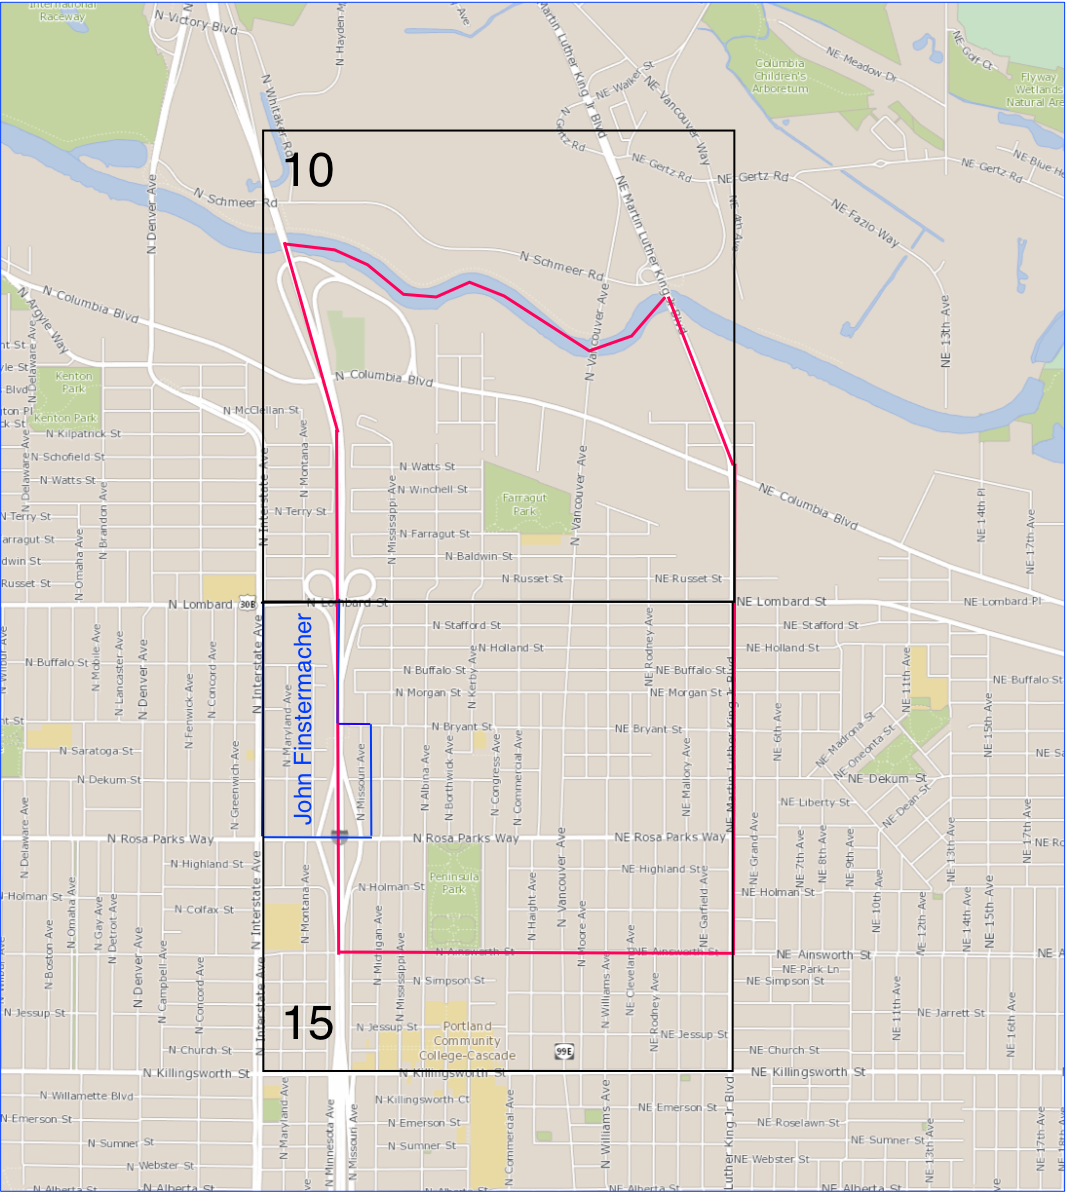
\includegraphics{images/0204a_images/image4.png}
\caption{alt\_text}
\end{figure}

\emph{\url{https://drive.google.com/open?id=1G9_RqgL55Ze2Uy4J2ls4kkrCqfnPU7cV}}

\begin{figure}
\centering
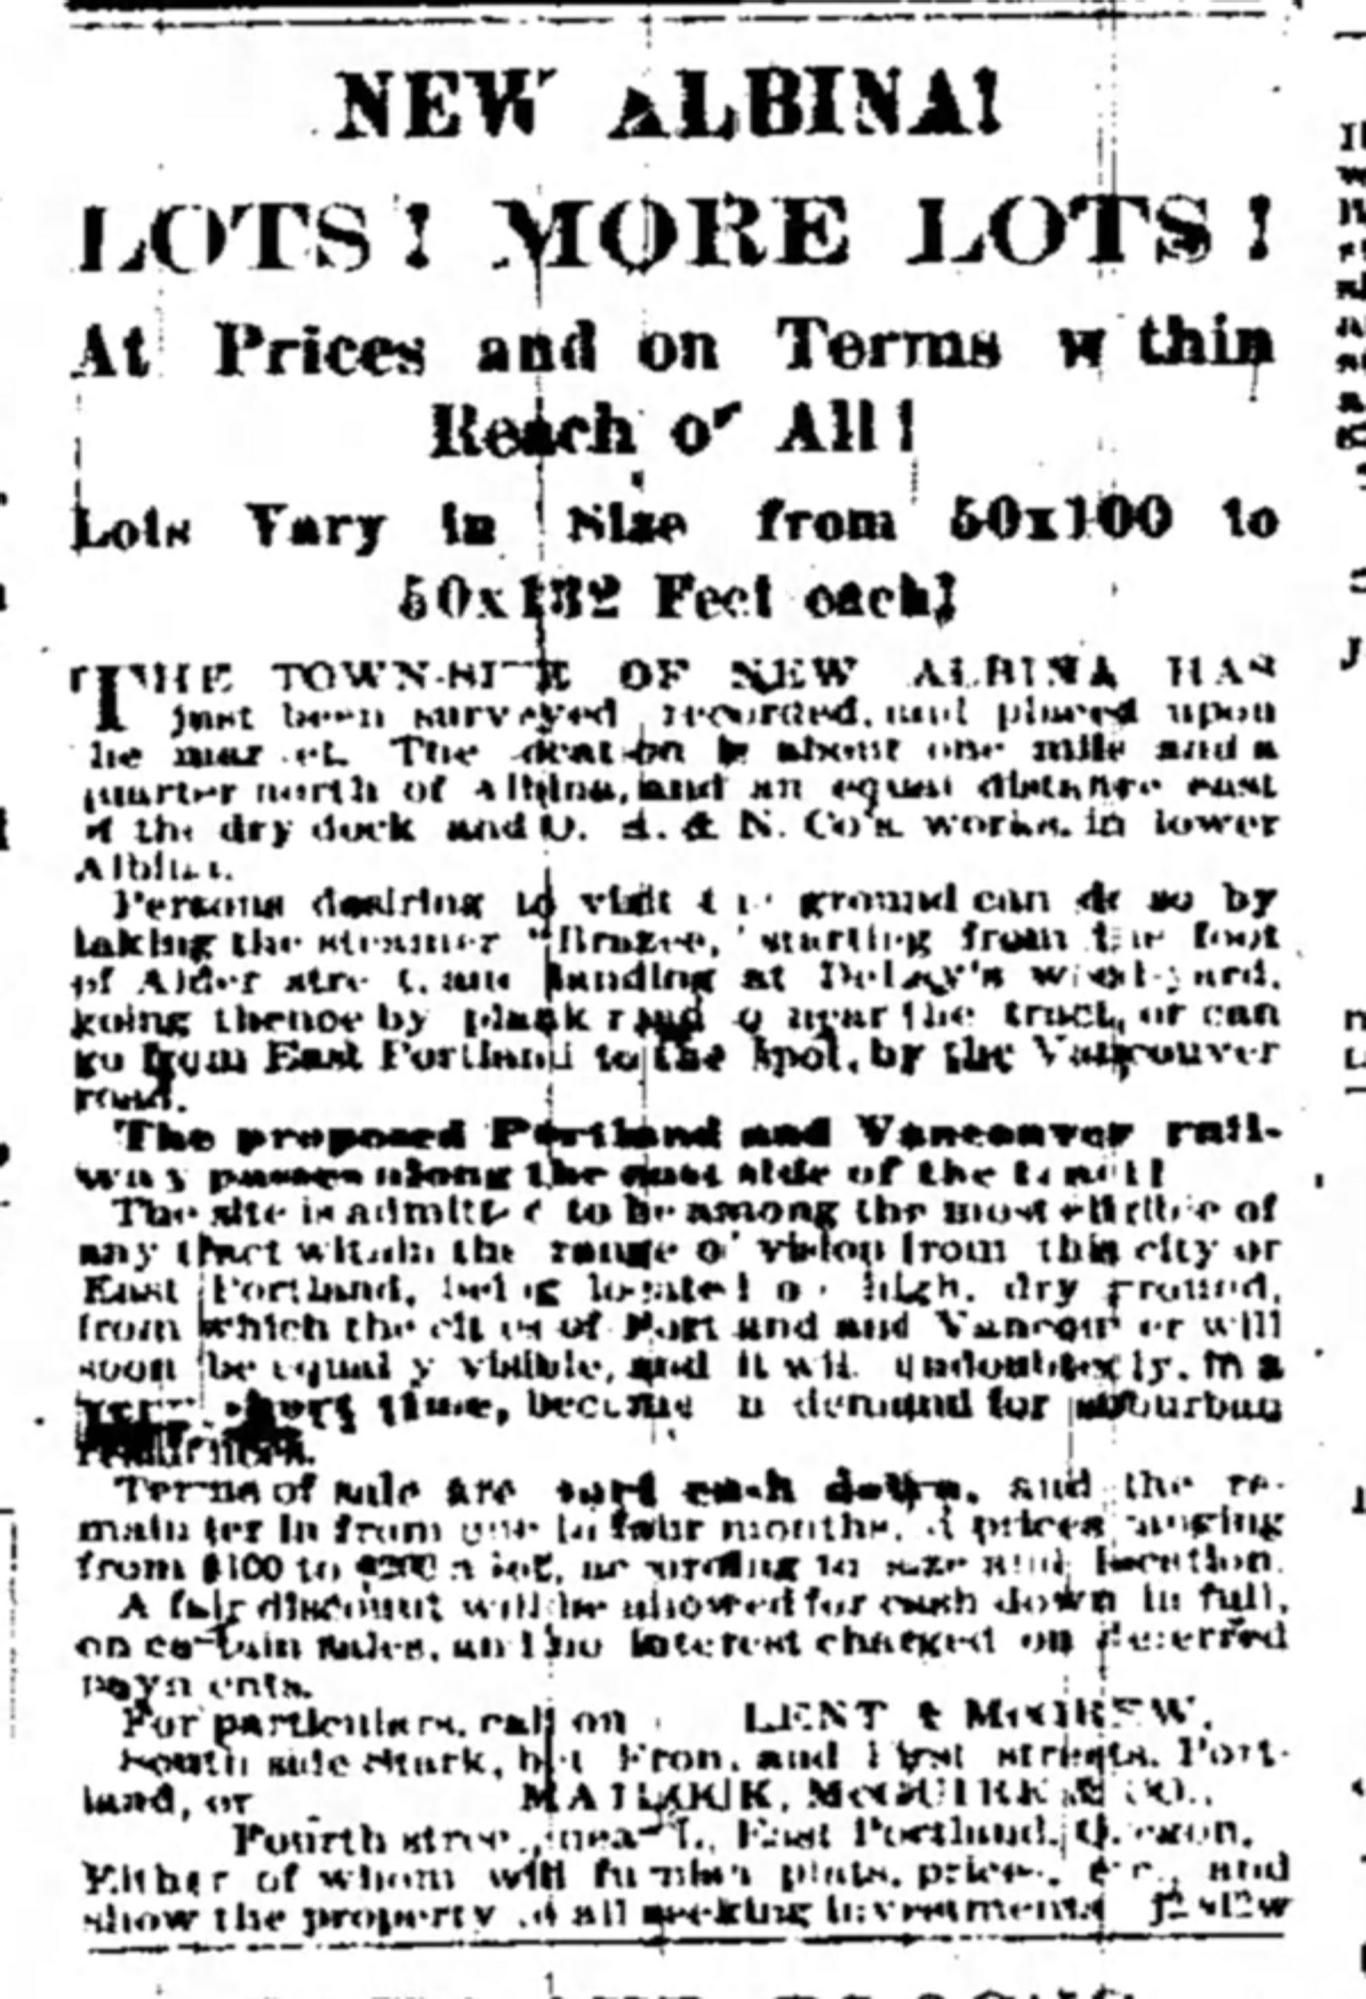
\includegraphics{images/0204a_images/image5.jpg}
\caption{alt\_text}
\end{figure}

\hypertarget{references-6}{%
\subsection{References}\label{references-6}}

Morning Oregonian 05/19/1887. \emph{A German Attempts Suicide by Cutting his Throat.}

\href{https://drive.google.com/file/d/0B94Urj3OjM7BVDNIR2FIU3lFZTA/view}{https://drive.google.com/file/d/0B94Urj3OjM7BVDNIR2FIU3lFZTA}

Morning Oregonian 05/09/1888. \emph{Property of a Dead Miser.}

\href{https://drive.google.com/file/d/100H41QRKIyYe9Fuf8c7yiTvqkH7_ieeX/view}{https://drive.google.com/file/d/100H41QRKIyYe9Fuf8c7yiTvqkH7\_ieeX}

Statesman Journal (Salem) 06/19/1887.\_ Committed Suicide.\_

\url{https://drive.google.com/open?id=12UsFogwBOdl0kJhVmU57KU_jWo1nIbr6}

Morning Oregonian 03/11/1890. \emph{The Fenstermacher Estate.}

\url{https://drive.google.com/file/d/14DmNJsic048rVIMugyFZUEOtAHmxDn46}

San Francisco Call 06/16/1897. \emph{Portland Heirs Sue for an Estate.}

\url{https://drive.google.com/file/d/1-IYGdy3n8UQQ0mDZg1Mq-W9t5Pd_ffOy}

Morning Oregonian 02/26/1898. \emph{More Heirs Turn Up.}

\emph{\url{https://drive.google.com/file/d/0B94Urj3OjM7BVERaOHlqTzZKdjA}}

Morning Oregonian 03/21/1898. \emph{More on Fenstermacher.}

\emph{\url{https://drive.google.com/file/d/0B94Urj3OjM7BVEpEdk80ZGd5NW8}}

Morning Oregonian 04/08/1898. \emph{One Set of Fenstermacher Claimants Retire from Litigation.}

\emph{\url{https://drive.google.com/file/d/0B94Urj3OjM7BVFBZRUJrNHVKYkk}}

Morning Oregonian 07/03/1898. \emph{Suite of Reputed Fenstermacher Heirs on Trial.}

\emph{\url{https://drive.google.com/file/d/0B94Urj3OjM7BVFBZRUJrNHVKYkk}}

Morning Oregonian 07/16/1898. \emph{Testimony in the Fenstermacher Suit Sifted.}

\emph{\url{https://drive.google.com/file/d/0B94Urj3OjM7BVFBZRUJrNHVKYkk}}

Morning Oregonian 09/20/1898. \emph{Decision in Fenstermacher Case Reached At Last.}

\emph{\url{https://drive.google.com/file/d/0B94Urj3OjM7BVFBZRUJrNHVKYkk}}

\emph{In re Petition of PETER FENSTERMACHER et al., Appellants, v. THE STATE OF OREGON, Respondent.} Reports of Cases Decided in the Supreme Court of the State of Oregon, Volume 19, p 504-508.

\emph{\url{https://drive.google.com/file/d/0B94Urj3OjM7BV3NRczdyVEFsbk0}}

\emph{Young et al.~v. State}. The Pacific Reporter, Volume 59, 1900, 812-814

\emph{\url{https://drive.google.com/file/d/0B94Urj3OjM7BV2J5YjhReWVXb2M}}

Statesman Journal (Salem). 03/03/1900 \emph{Long Drawn-Out Litigation.}

\emph{\url{https://drive.google.com/open?id=1vhwqpATluytKALr6fzlN3aOgnccoJXo6}}

Ancestry.com. \emph{U.S., Revolutionary War Pension and Bounty-Land Warrant Application Files, 1800-1900 }{[}database on-line{]}. Provo, UT, USA: Ancestry.com Operations, Inc., 2010.

\emph{\url{https://drive.google.com/file/d/1-3Rs-_x_Ol7FVXFutx9VwanH0kxq1xzx}}

Ancestry.com. \emph{U.S., Civil War Draft Registration Records 1863-1865 }{[}database on-line{]}. Provo, UT, USA: Ancestry.com Operations, Inc., 2010.

\emph{\url{https://drive.google.com/open?id=1RcUv1nvTcXDlx2JBSKsxeNAYsrr6SSAQ}}

Genealogical Forum of Oregon: \emph{The Oregonian-News from East Portland, 1880s}

\emph{\url{http://gfo.org/resources/indexes/other-indexes/east-portland-news.html}}

Eugene E. Snyder: \_We Claimed this Land: Portland's Pioneer Settlers. \_Binfort \& Mort Publishing, Portland, Oregon, 1989

\emph{Draft Albina Community Plan Context Statement}, Portland Bureau of Planning, 1993

Multnomah County Court, \emph{Probate Case 1369, Estate of John Finstamacher.}

\url{https://drive.google.com/open?id=15hQltM24BGUZjA6WXPmCE0vb6i8jHsgg}

\hypertarget{homesteaders-john-fenstermacher}{%
\section{Homesteaders: John Fenstermacher}\label{homesteaders-john-fenstermacher}}

\hypertarget{death-1}{%
\subsection{Death}\label{death-1}}

{\textgreater\textgreater\textgreater\textgreater\textgreater{} gd2md-html alert: inline image link here (to images/image1.jpg). Store image on your image server and adjust path/filename/extension if necessary. }(Back to top)(Next alert){\textgreater\textgreater\textgreater\textgreater\textgreater{} }

\begin{figure}
\centering
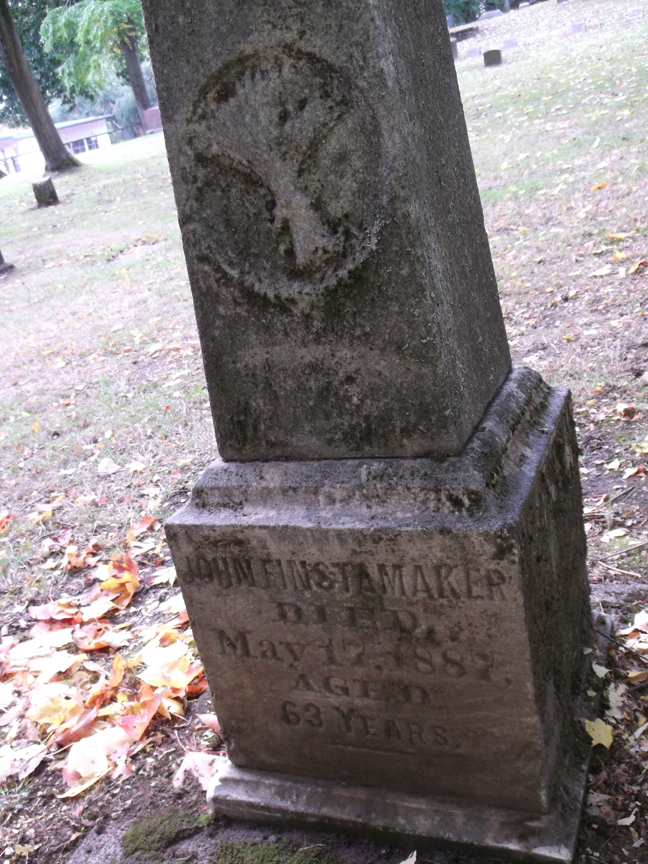
\includegraphics{images/0204b_images/image1.jpg}
\caption{alt\_text}
\end{figure}

Before I am going to discuss what I know about John Fenstermachers life, I first have to mention that his last name is often spelled differently, for instance Findsermacker or Finstamaker. And various permutations of these variations. Because of later developments, discussed below, I will use Fenstermacher. Snyder (1989, p 80-81) suggests the different spellings are there because Fenstermacher did not know how to write. No matter how you spell it, it means windowmaker. It suggests an Amish or Pennsylvania Dutch origin, and indeed there are many Fenstermachers in Pennsylvania. But, like for his homesteading neighbor Evander Howe, initially the details about John Fenstermacher's life are scarce and hard to come by. As is often the case, as we saw with both Liverpool Liz and Evander Howe, information becomes more readily available at death.

Probate file.

So let us look into the sad death of John Fenstermacher. He died May 17, 1887, and was buried in Lone Fir Cemetery, section 19, lot 26, grave 2S. The excellent Find-a-Grave site has a picture of the gravestone, which also tells me he was 63 years old when he died, leading us to believe he was born in 1824.

\begin{quote}
\emph{His grave is in Lone Fir Cemetery, marked by a weathered shaft of marble with one simple decoration, a bundle of wheat -- reference to the Biblical assurance that ``He will gather His wheat unto Himself'' (Snyder, 1989, p.~81).}
\end{quote}

Of course the gravestone does not tell us how he died, or who paid for the obelisk and the grave site. My guess is it was paid for by the State of Oregon, which was, at least initially, the beneficiary of his death.

Next on my search I found two articles from the Morning Oregonian, the first from May 19, 1887, and the second from May 9, 1888. I summarize their story, which has some temporal peculiarities. Remember the official date of death is May 17, 1887. Here is the first article.

\begin{figure}
\centering
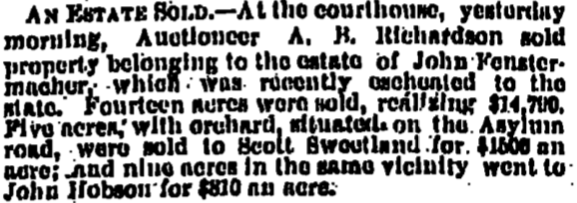
\includegraphics{images/0204b_images/image2.png}
\caption{alt\_text}
\end{figure}

The article says that ``yesterday'' John Fenstermacher tried to commit suicide by cutting his throat with a razor at his own residence on Asylum Road. Let's assume that ``yesterday'' is, indeed, May 17, 1887. W. F. McMonies, a neighbor, found him and eventually got him to Dr.~Coley who dressed his wounds.

\begin{quote}
\emph{After his wounds were dressed he was able to talk readily, and told the doctor he had committed the rash act on account of being disappointed in a love affair. }
\end{quote}

The second article of May 9, 1888 says that on May 17, 1887 the second suicide attempt, this time by hanging, was successful. This obviously corresponds with the official date of death. The article says

\begin{quote}
\emph{Previously he made an attempt on his life by cutting his throat. }
\end{quote}

Snyder (1987, p.~80) has a lurid account of the two suicide attempts. In fact, he even describes a third attempt, also involving a razor, and for both failed attempts he gives the names of the doctors, and even the amount of their bills. I am not sure where that information comes from, because of Snyder's infuriating habit not to give references and sources, and to be rather cavalier about names and dates. Again, his books are very useful, but they would have been so much more useful with suitable notes and references. Anyway, let's copy here what Snyder says on his page 80.

\begin{quote}
\emph{Lying in a pool of blood with his throat cut, John Finstamaker (or Findermacker -- his name was spelled various ways because he did not know how to write) was found in his bachelor's farmhouse one day in the spring of 1887 by a neighbor, William Monies. John was still alive, so Monies got him into a buggy and whipped off to try to find a doctor before the victim bled to death. He had to drive to various offices before finding a doctor in. ``At last,'' as Monies said in his account of the incident, he found a Dr.~Coles, who ``operated on the cut neck, charging \$50.''}
\end{quote}

\begin{quote}
\emph{This was the second time John had tried to commit suicide. The first time Dr.~John Sellwood had repaired the damage for \$ 25. But the third time was the charm. John died by his own hand May 17, 1887, and, hopefully, found the piece he was seeking. He was 63 years old. What disappointments, what self-recrimination, regrets or remorse may have tortured poor old John, God alone knows. }
\end{quote}

Not just God, it turns out. Fenstermacher told the reporter of the Oregonian that he was ``disappointed in a love affair''. Snyder also has the names of the doctor, of the victim, and of the neighbor wrong, or at least different from what the Oregonian has. In subsequent remarks on the Fenstermacher inheritance and relatives he also makes various mistakes, so I am not sure about the veracity of what he describes as the first attempt.

Also note that according to the information we have so far, Fenstermacher cut his throat in May 17, then was taken to Good Samaritan, and then hung himself on the same day. This seems an unlikely sequence of events. For a more plausible story we rely on information from the Statesman Journal of June 19, 1887.

\begin{figure}
\centering
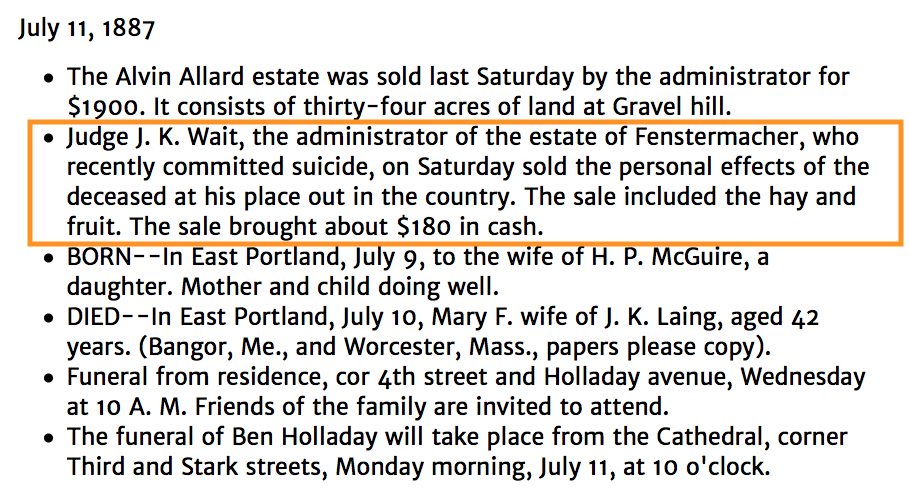
\includegraphics{images/0204b_images/image3.png}
\caption{alt\_text}
\end{figure}

This suggests Fenstermacher was committed after his suicide attempt, did some gardening on the hospital grounds for a month, and then hung himself on June 17, 1887. It implies, of course, that the official day of death, which is on the grave in Lone Fir, is incorrect. Whoever paid for the grave used the first suicide date as the day of death -- but Fenstermacher managed to live another month after his official death.

Be that as in may, the second Oregonian article of May 9, 1888 gives some interesting personal details, probably gathered from neighbors and other acquaintances. Fenstermacher came to Oregon as a private in the US Army, and fought under Sheridan in a battle with Indians at the Cascades. After his death his personal property was found buried in various places. He had also mentioned to these same acquaintances or neighbors that he made several substantial deposits, but because he did not mention in which bank, they could not be found.

\begin{quote}
\emph{He was a miserly person, never known to expend a cent unnecessarily; and some who knew him intimately say that in his greed for wealth, he even deprived himself of sufficient to eat.}
\end{quote}

In addition

\begin{quote}
\emph{He never spoke of himself or family relations, and no one here ever knew from whence he came, hence, after his death, all efforts to learn as to whether of where he had lawful relatives were unavailing, although no little trouble was taken in the premises.}
\end{quote}

As a result of all this secretiveness there was no testament to be found. Fenstermacher died intestate, and his estate, worth \$ 15,000, by law escheated to the State of Oregon on May 20, 1888. Note that inflation calculators tell us that \$ 15,000 in 1887 dollars is \$ 375,000 in 1917 dollars. A considerable amount of money, to be sure. Also, in the Notes from East-Portland, on the site of the Genealogical forum of Oregon, we find the following clipping.

\begin{figure}
\centering
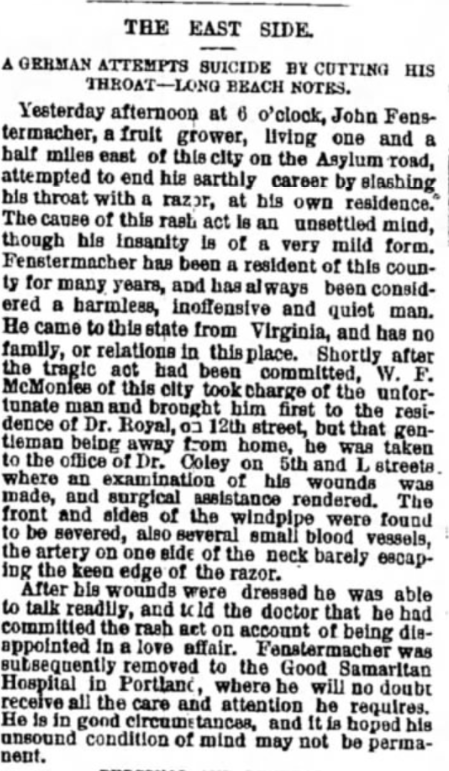
\includegraphics{images/0204b_images/image4.png}
\caption{alt\_text}
\end{figure}

And in the Morning Oregonian of June 19, 1888 we see how the state disposed of the Fenstermacher land in East Portland.

\begin{figure}
\centering
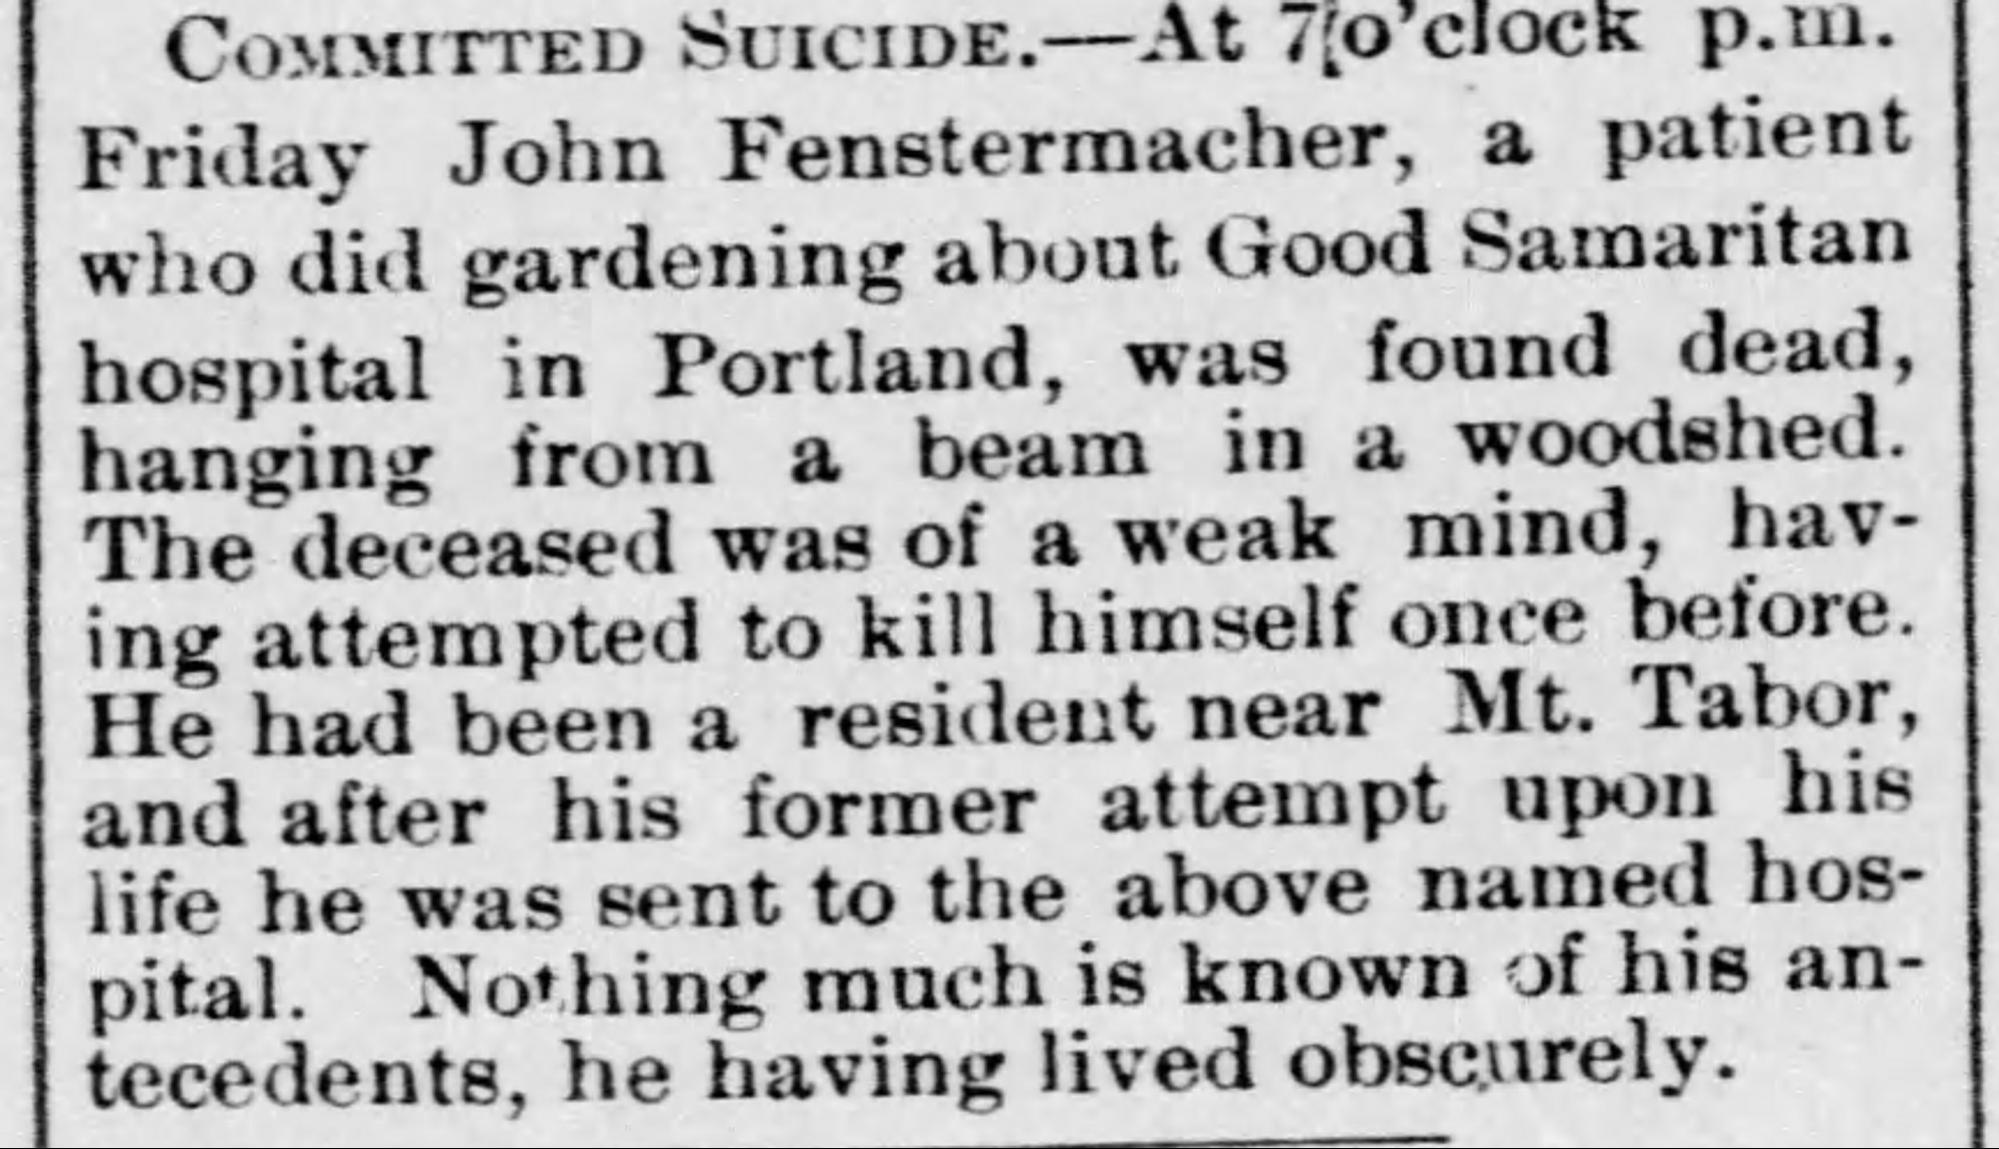
\includegraphics{images/0204b_images/image5.jpg}
\caption{alt\_text}
\end{figure}

Just for completeness, here are the two deeds. First State of Oregon to Svetland

\url{https://drive.google.com/open?id=1Yfi9f7CFIhlfu4t7IdbEwe80zBAszlfu}

And then State of Oregon to Hobson

\url{https://drive.google.com/open?id=1ShOldKWWl6DtrqTjBwCFL5HQnihO_-E2}

\hypertarget{the-heirs}{%
\subsection{The Heirs}\label{the-heirs}}

After 1888 all should have gone quiet. But it didn't. News of Fenstermacher's death, and of the large amount of money sitting in the state's coffers, soon reached Pennsylvania. And these alleged relatives, or their lawyers, flocked to Oregon to sue the state and to prove to the courts they were indeed the legal heirs. It is not easy to disentangle all these lawsuits, but I shall try. In the process a lot of new information about John Fenstermacher will come to the fore.

The first case was filed in Multnomah Circuit Court by Peter Fenstermacher et al.~on May 25, 1889. Judge Stearns appointed Mr.~George A. Brodie to investigate their claims. I am not sure what Mr.~Brodie found, but the court ruled the plaintiffs were not the relatives of John Fenstermacher. On March 10, 1890 Judge A. H. Tanner represented another batch of alleged heirs in the same court. He asked to send a commissioner to Pennsylvania to ``take testimony''.

Judge Stearns said he had already made his ruling in the previous case, and ``further proceedings in the matter must be carried to the supreme court''. On October 27, 1890 the Oregon Supreme Court refused to overrule the circuit court's decision.

Skip to 1897. In the San Francisco Call of June 16, 1897 it is reported that 67 Fenstermacher relatives, represented by the firm of Emmons \& Emmons, began suit in the Multnomah Circuit Court. In connection with this suit

\begin{quote}
\emph{Attorney Chester A. Dolph was commissioned by Governor Lord to go East and investigate the claim, and his report was adverse to the heirs.}
\end{quote}

The Morning Oregonian of April 8, 1898 mentions that Judge Sears dismissed the suit, of

Alice Reonbault et al.~vs the State Of Oregon, because Emmons \& Emmons failed to produce two witnesses

\begin{quote}
\emph{\ldots{} of which one -- J. Schaefer -- has died since the action was begun, and the other -- Harry Monice -- has gone to the Klondyke.}
\end{quote}

The article also mentions another suit going on, championed by Attorney J.C. Moreland, ``who is now East gathering testimony''. More detail about this latest lawsuit is in the Morning Oregonian of February 28, 1898. Plaintiffs are Amos L. Young, Charles W. Young, Sue Osterman, Mary Osterman, and Elizabeth Osterman. Amos and Charles Young maintained they were sons of Lavina Fenstermacher, a sister of John Fenstermacher. The Osterman women were daughters from a second marriage of John Fenstermacher's mother.

\begin{quote}
\emph{Mary Osterman and Elizabeth Osterman are of unsound mind, and J.C. Moreland has been appointed their guardian ad litem.}
\end{quote}

The article briefly summarizes the proceedings in the earlier lawsuits in Judge Stearns' court.

\begin{quote}
\emph{At the time of this suit several attorneys went to Pennsylvania, and found the Fenstermachers were a very prolific race, and thick as fleas in that state, but none of them could establish relationship with this Fenstermacher.}
\end{quote}

Some additional information was provided by these alleged relatives about John Fenstermacher. He enlisted in the army in Pennsylvania, and then came west with his regiment to Walla Walla. He had a tendency ``for deserting from the army every now and then''. This was supposedly born out by army records. It made me curious. There is a 1873 army pension application, under number R. 3,524, for service in Pennsylvania by John Fenstermacher, which was actually rejected, perhaps because of later desertions. Ancestry.com also has a June 1863 civil war draft registration record from the counties of Schuylkill and Lebanon in Pennsylvania, where John Fenstermacher, 39 years old, a merchant, is declared eligible for the draft.

\begin{figure}
\centering
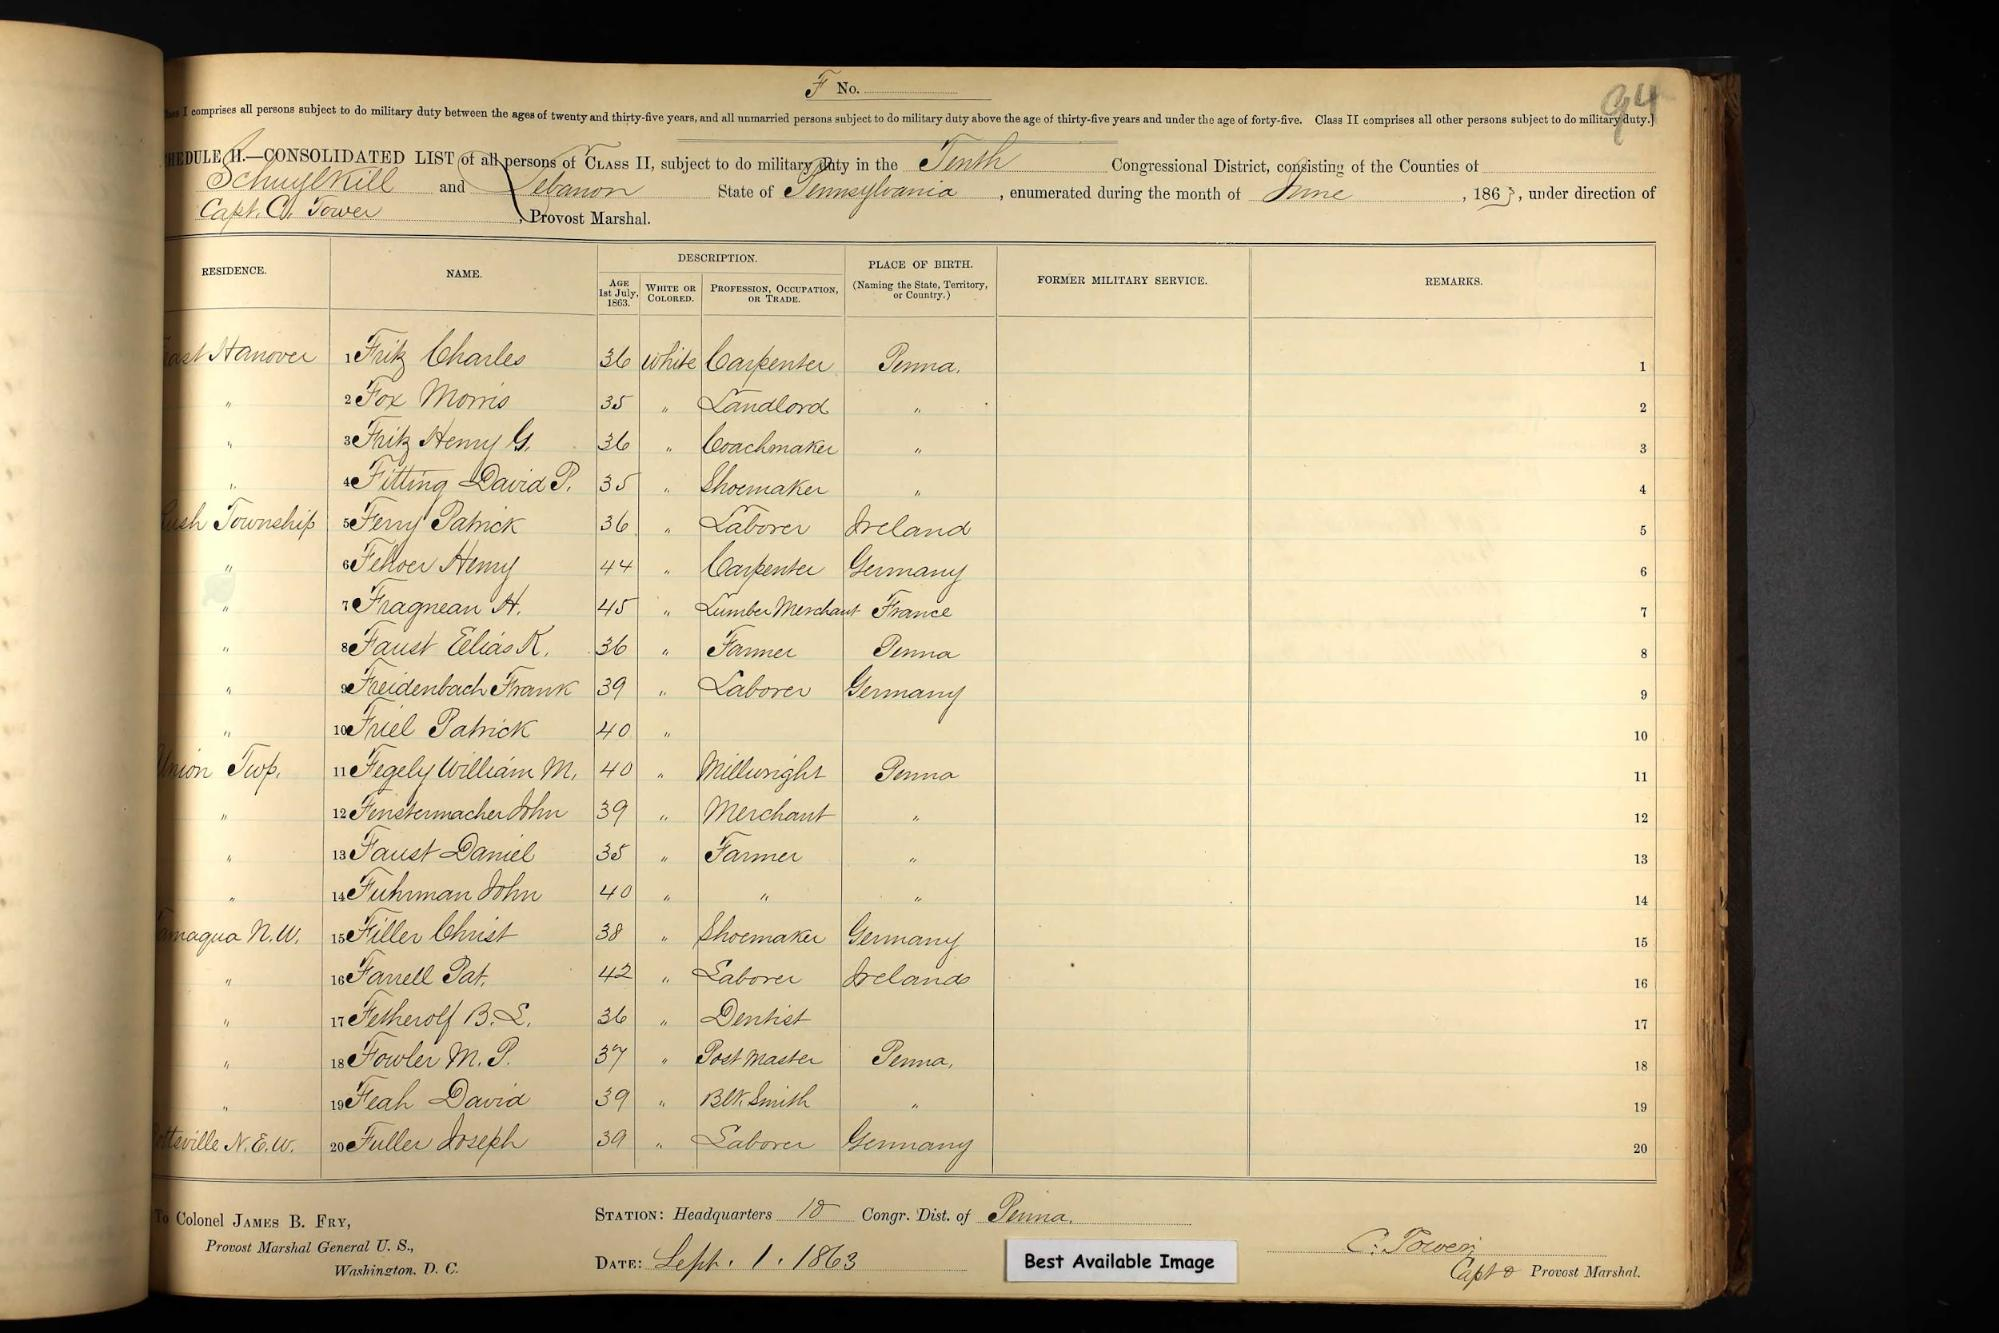
\includegraphics{images/0204b_images/image6.jpg}
\caption{alt\_text}
\end{figure}

\url{https://drive.google.com/open?id=1RcUv1nvTcXDlx2JBSKsxeNAYsrr6SSAQ}

The Morning Oregonian of March 21, 1898 made some coastal elitist fun of the simple souls in Pennsylvania. They got hold of a March 5th, 1898 letter from a Mrs.~Amanda Laubach, from Kreidersville, Northampton County, Pa., addressed to ``Any Postmaster in the State of Oregon''.

\begin{quote}
\emph{Mr Jehtelmen}
\end{quote}

\begin{quote}
\emph{Will you Pleas and Let me no if John Fenstermacher is Died in the State of Oregon. If not ask the Justice of the Peace if you Pleas. We Se in the Paper that John Fenstermach Died and left a big estate. He Disappeared From here in 1858 Where he bought an Ammence tract of land. He died a hermit. I will give you some of the Fenstermacher Name.}
\end{quote}

The Oregonian continues

\begin{quote}
\emph{Then follows a list of names as long as the list of patriarchs given in the fifth chapter of Genesis, and which might be as interesting, if it only stated how long each Fenstermacher lived and whom he begat.}
\end{quote}

Unlike the previous lawsuits, this last one had legs. Attorney J.C. Moreland had done his homework, and produced a long string of witnesses. The state, in the person of Attorney Chester V. Dolph, also put up a fight. Before we go into the arguments, we may as well summarize the Fenstermacher story, as argued by the plaintiffs. The clearest statement is in the Pacific Reporter, from when the case reached the Supreme Court.

\begin{quote}
\emph{To prove their heirship, they gave evidence to the effect that in 1826 or 1827 one George Fenstermacher and Elizabeth Newhard were married in Pennsylvania, and as a result of such marriage four children were born to them, to wit, LaVina, Jonas, Amanda, and John; the two latter of whom died at an early age, unmarried. About 1837 or 1838 the father deserted the family, and was never afterwards heard of. Lavina, the eldest daughter, then a girl 10 or 11 years of age, went out to work, and was subsequently married to John Young, a stage driver, by whom she had three children, one of whom died in infancy, and the other two are plaintiffs in this action. The mother, Elizabeth, with her two sons, after living among her relatives a short time, went to the Northampton poor house in 1839. From there Jonas was bound out to one David Keller of Stroudsburg, Pa., where he remained five or six years. He then went to learn the brick mason's trade with a man by the name of Deal, with whom he remained a short time, and then went away to shift for himself. After remaining at the poor house for a time, his mother married one Osterman, by whom she had three children, who are also plaintiffs in this case. She died July 22, 1889. }
\end{quote}

Single mother, poor house, son given in bondage, two daughters judged to be ``insane'' from a second marriage. Just to be complete I checked the Federal Census in Pennsylvania. In the 1850 Census in Denison, Luzerne, Pa., we find Lavina Young (23), married to John Young (28), with children Elizabeth (6), and Amos T. (2). In the 1860 Census in Lausanne, Carbon, Pa., we find Domnick Osterman (53), married to Osterman (no first name, 52), with children Susan (17), Joseph (13), Elizabeth (10), and Mary (7). Those are our plaintiffs, all right.

The story continues with Jonas Fenstermacher's military career, illustrating why he was denied a civil war pension.

\begin{quote}
\emph{The plaintiff's further gave evidence to the effect that in June, 1855, a young man calling himself John Fenstermacher enlisted at Wilkesbarre, Pa., in Company G, 9th regiment, United States infantry, and afterwards came with his company to this coast. After he enlisted he was arrested, or his arrest attempted, on a warrant under the name of Jonas Fenstermacher; but by some arrangement or management of the captain the officer was not allowed to take him, and he went on with his company. At Ft. Simcoe, about 1858 or 1859, he was accused of desertion, caught, flogged, and dishonorably discharged.}
\end{quote}

Five years later he was in Portland, bought and sold various pieces of land, grew fruit and raised cattle on Asylum Road, lead a lonely and miserly life, and managed to scrape together a small fortune. But eventually the demons from his past got the better of him, and in a second or third attempt he killed himself.

From Polk's Portland City Directories we find that in 1885, 1886, and 1887 John Fenstermacher lived on Asylum Road. In 1885 he was listed as a farmer, in 1886 and 1887 as a fruit grower.

Asylum Road in East Portland used to be named U Street. In 1859 Dr.~J.C. Hawthorne started the private Oregon Hospital there. It soon started to specialize in the treatment of mental illness, and in 1862 it became Oregon Hospital for the Insane, the first such facility in the state. By 1873 18-20 percent of the population of East Portland worked there, and U Street was renamed Asylum Street. Most patients were committed by the state, and the hospital was almost exclusively funded by Dr.~Hawthorne's lucrative state contract. His friends in high places supported him until well in the 1880's, when the state mental hospital moved to Salem. The distastefully named Asylum Road became Hawthorne Avenue. What upstanding citizen would want to buy a house on Asylum Road ?

In the San Francisco Call of June 16, 1897 it says Fenstermacher lived on 14 acres he owned in the Seldon and Hiantha Murray Donation Land Claim, which means he grew his fruit somewhere on what is now Hawthorne Boulevard between 20th and 38th Street. Those are the 14 acres sold by the state in June 1888.

In the lawsuit the various witnesses for the plaintiffs testified that they knew Jonas or John Fenstermacher in Pennsylvania or in the military, and that he had told them the various details of his life. Attorney Dolph argued that the case was completely based on hearsay, because the witnesses had all their information from Fenstermacher himself, who was now deceased. The state argued that there indeed was a Jonas Fenstermacher in Pennsylvania, and in the US Army, but it had not been established that this was the same person as the John Fenstermacher who died in Portland.

On September 19, 1898 Judge Sears sided with the plaintiffs, and awarded them the fund. One last thing had to be settled.

\begin{quote}
\emph{The evidence shows the original amount of the escheated assets to have been \$ 15,165.62, but that the state has paid out \$ 1,995.05 for costs and expenses necessarily incurred in successfully defending two certain actions brought to recover the fund by parties claiming to be entitled thereto.}
\end{quote}

Attorney Moreland and the plaintiffs did not like the fact that they had to pay the state for the costs of the failed lawsuits of their relatives, and appealed that part of the ruling. The Supreme Court of Oregon on January 29, 1900 decided to uphold Judge Sears' calculations. As in the previous Peter Fenstermacher et al.~appeal, the Supreme Court refused to rule on the facts of the case, because ``a proceeding of this kind is an action at law, and therefore the findings of the trial court upon controverted facts are not open to review here.'' The lawsuits were finally settled.

\begin{figure}
\centering
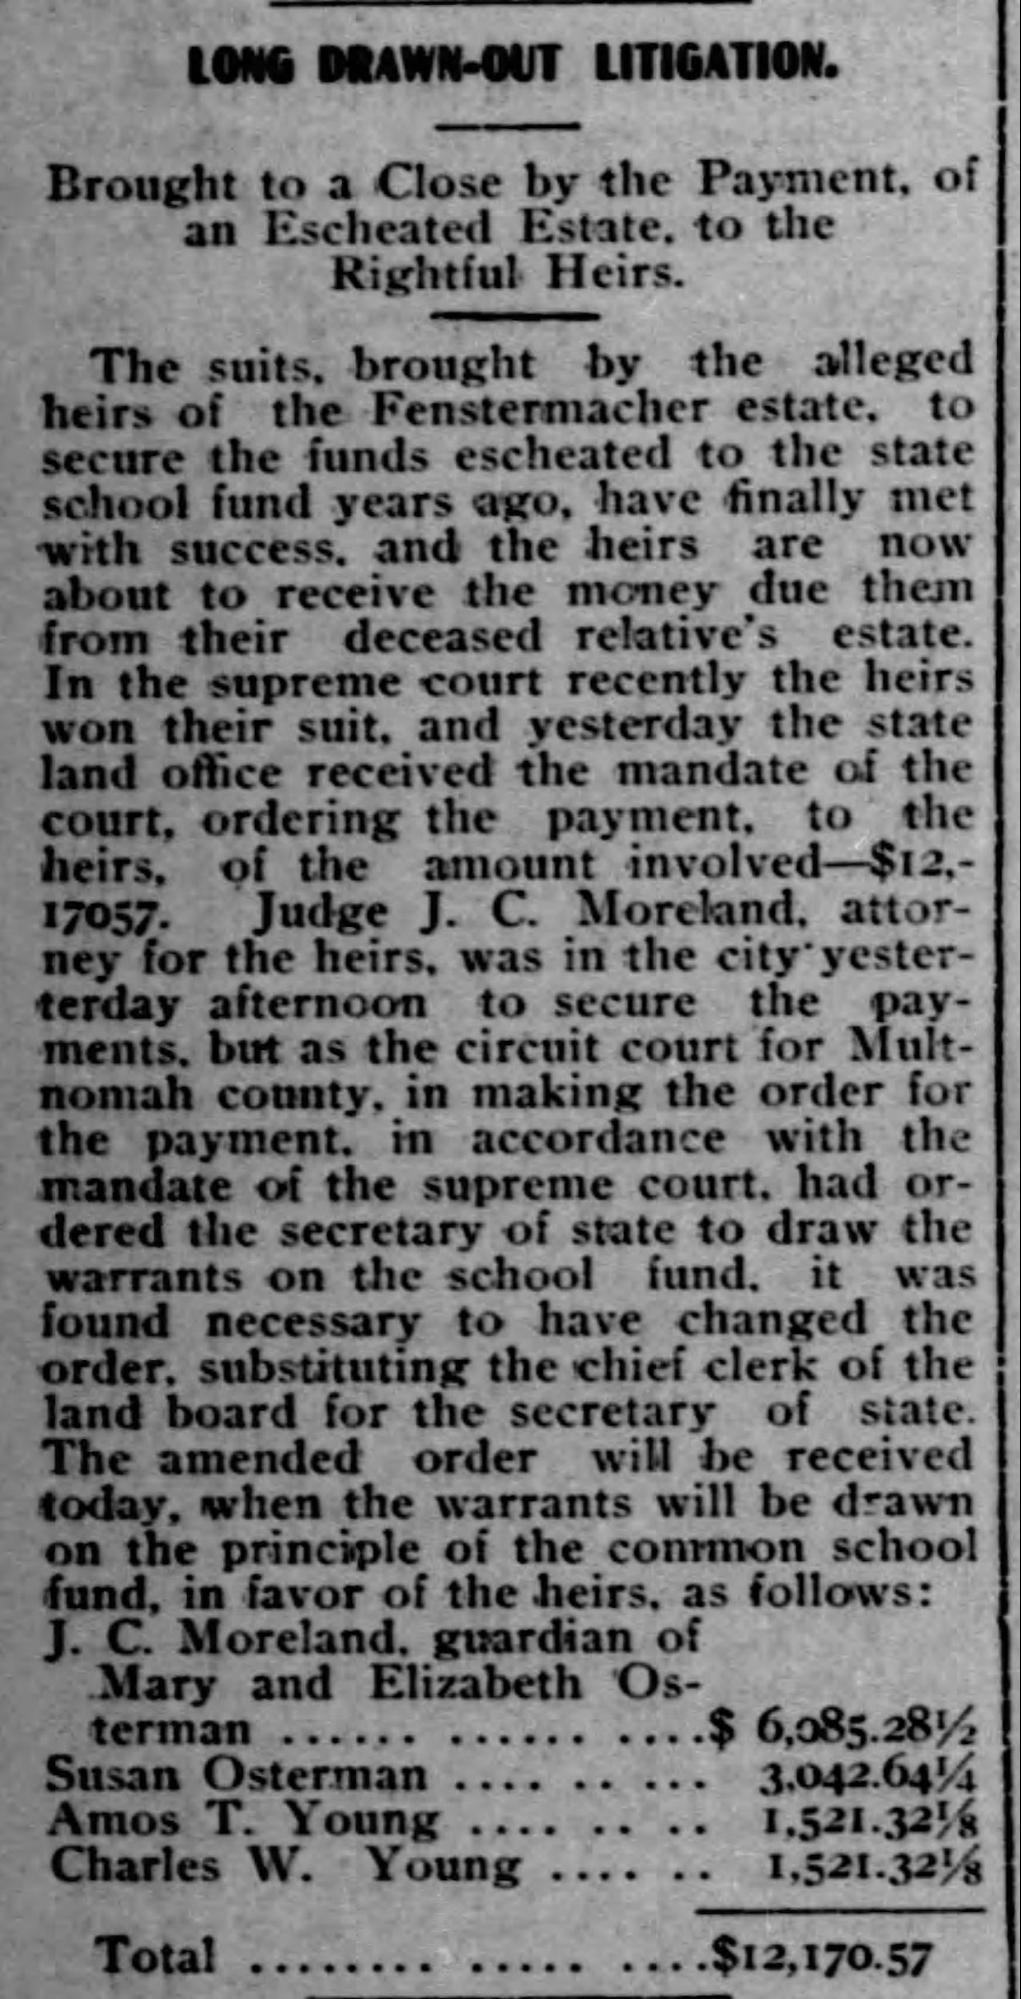
\includegraphics{images/0204b_images/image7.jpg}
\caption{alt\_text}
\end{figure}

Thus ends the sad story of Jonas Fenstermacher, who very briefly owned a very small part of the Piedmont Neighborhood, and of the hundreds of relatives who wanted a piece of the estate when he died.

\hypertarget{references-7}{%
\subsection{References}\label{references-7}}

Morning Oregonian 05/19/1887. \emph{A German Attempts Suicide by Cutting his Throat.}

\href{https://drive.google.com/file/d/0B94Urj3OjM7BVDNIR2FIU3lFZTA/view}{https://drive.google.com/file/d/0B94Urj3OjM7BVDNIR2FIU3lFZTA}

Morning Oregonian 05/09/1888. \emph{Property of a Dead Miser.}

\href{https://drive.google.com/file/d/100H41QRKIyYe9Fuf8c7yiTvqkH7_ieeX/view}{https://drive.google.com/file/d/100H41QRKIyYe9Fuf8c7yiTvqkH7\_ieeX}

Statesman Journal (Salem) 06/19/1887.\_ Committed Suicide.\_

\url{https://drive.google.com/open?id=12UsFogwBOdl0kJhVmU57KU_jWo1nIbr6}

Morning Oregonian 03/11/1890. \emph{The Fenstermacher Estate.}

\url{https://drive.google.com/file/d/14DmNJsic048rVIMugyFZUEOtAHmxDn46}

San Francisco Call 06/16/1897. \emph{Portland Heirs Sue for an Estate.}

\url{https://drive.google.com/file/d/1-IYGdy3n8UQQ0mDZg1Mq-W9t5Pd_ffOy}

Morning Oregonian 02/26/1898. \emph{More Heirs Turn Up.}

\emph{\url{https://drive.google.com/file/d/0B94Urj3OjM7BVERaOHlqTzZKdjA}}

Morning Oregonian 03/21/1898. \emph{More on Fenstermacher.}

\emph{\url{https://drive.google.com/file/d/0B94Urj3OjM7BVEpEdk80ZGd5NW8}}

Morning Oregonian 04/08/1898. \emph{One Set of Fenstermacher Claimants Retire from Litigation.}

\emph{\url{https://drive.google.com/file/d/0B94Urj3OjM7BVFBZRUJrNHVKYkk}}

Morning Oregonian 07/03/1898. \emph{Suite of Reputed Fenstermacher Heirs on Trial.}

\emph{\url{https://drive.google.com/file/d/0B94Urj3OjM7BVFBZRUJrNHVKYkk}}

Morning Oregonian 07/16/1898. \emph{Testimony in the Fenstermacher Suit Sifted.}

\emph{\url{https://drive.google.com/file/d/0B94Urj3OjM7BVFBZRUJrNHVKYkk}}

Morning Oregonian 09/20/1898. \emph{Decision in Fenstermacher Case Reached At Last.}

\emph{\url{https://drive.google.com/file/d/0B94Urj3OjM7BVFBZRUJrNHVKYkk}}

\emph{In re Petition of PETER FENSTERMACHER et al., Appellants, v. THE STATE OF OREGON, Respondent.} Reports of Cases Decided in the Supreme Court of the State of Oregon, Volume 19, p 504-508.

\emph{\url{https://drive.google.com/file/d/0B94Urj3OjM7BV3NRczdyVEFsbk0}}

\emph{Young et al.~v. State}. The Pacific Reporter, Volume 59, 1900, 812-814

\emph{\url{https://drive.google.com/file/d/0B94Urj3OjM7BV2J5YjhReWVXb2M}}

Statesman Journal (Salem). 03/03/1900 \emph{Long Drawn-Out Litigation.}

\emph{\url{https://drive.google.com/open?id=1vhwqpATluytKALr6fzlN3aOgnccoJXo6}}

Ancestry.com. \emph{U.S., Revolutionary War Pension and Bounty-Land Warrant Application Files, 1800-1900 }{[}database on-line{]}. Provo, UT, USA: Ancestry.com Operations, Inc., 2010.

\emph{\url{https://drive.google.com/file/d/1-3Rs-_x_Ol7FVXFutx9VwanH0kxq1xzx}}

Ancestry.com. \emph{U.S., Civil War Draft Registration Records 1863-1865 }{[}database on-line{]}. Provo, UT, USA: Ancestry.com Operations, Inc., 2010.

\emph{\url{https://drive.google.com/open?id=1RcUv1nvTcXDlx2JBSKsxeNAYsrr6SSAQ}}

Genealogical Forum of Oregon: \emph{The Oregonian-News from East Portland, 1880s}

\emph{\url{http://gfo.org/resources/indexes/other-indexes/east-portland-news.html}}

Eugene E. Snyder: \_We Claimed this Land: Portland's Pioneer Settlers. \_Binfort \& Mort Publishing, Portland, Oregon, 1989

\emph{Draft Albina Community Plan Context Statement}, Portland Bureau of Planning, 1993

Multnomah County Court, \emph{Probate Case 1369, Estate of John Finstamacher.}

\url{https://drive.google.com/open?id=15hQltM24BGUZjA6WXPmCE0vb6i8jHsgg}

\hypertarget{references-8}{%
\chapter*{References}\label{references-8}}
\addcontentsline{toc}{chapter}{References}

\end{document}
